\documentclass[isdraft]{kclthesis}  % notes see below
									% [releaseproject] will check release,
							 		% [notreleaseproject] will check not release.
							 		% [isdraft] provides background water mark "DRAFT"
							 		% [kclharvardbib] provides different reference style.

% glossaries


% Run texcount on tex-file and write results to a sum-file
\immediate\write18{texcount \jobname.tex -merge -total | grep "Words in text: " | cut -d" " -f4 > \jobname.sum}
% Define macro \wordcountsum for including the counts
\newcommand\wordcountsum{\input{\jobname.sum}}


\newenvironment{markdown}%
    {\VerbatimEnvironment\begin{VerbatimOut}{tmp.markdown}}%
    {\end{VerbatimOut}%
        \immediate\write18{pandoc tmp.markdown -t latex -o tmp.tex}%
        \input{tmp.tex}}
\def\tightlist{}


\usetikzlibrary{shapes}
\setlist{nosep} % or \setlist{noitemsep} to leave space around whole list


% customize your general setup here
\title{Automated Small Datanalyst}
\author{Sebastian Zillessen}
\modulecode{7CCSMPRJ}
\submissiontitle{Individual Project Submission 2015/16}
%\submissiontitle{Preliminary Project Report}
\studentnumber{\#1564629}
\programme{MSc Web Intelligence MSc}
\supervisor{Jeroen Keppens}
\cosupervisor{Isabel Sassoon}
\department{Department of Informatics}
\wordcount{ \wordcountsum }
% 15000 words (excluding Cover page, Acknowledgement, Table of contents, Nomenclature, List of figures and tables, References, Appendix)


%\makenomenclature
\makeglossaries


\pretocmd{\section}{\glsresetall}{}{}


\begin{document}


\pagenumbering{gobble}

%TC:ignore
%%%%%% depends what you like, might try out the other frontpage as well
\maketitle 		% official styled layout
\maketitleTwo 	% adapted layout which looks nicer from my point of view.

%%%%%% empty page after main page.
\newpage
\thispagestyle{empty}
\mbox{}
\newpage
%%%%%% Abstract
%TC:endignore

%TC:break Abstract
\section*{Abstract}

Data collection has seen a dramatic increase over the last years and researchers agree exploiting these to create data driven decision processes is crucial to generate valuable insights for clinical studies. This generates the requirement to assist clinicians during the design process of their studies with an intelligent support agent performing these analyses for them. 

This project looks at an existing approach to apply argumentation on this problem, by representing the statistical models and their assumptions as a statistical knowledge base and implementing the process into a user-friendly web application. The model selection is influenced by expressing preferences applying on different context domains and the close integration of the clinician and insights she/he can give related to the process. This will enable clinicians -- even without a background in statistics or informatics -- to answer their research questions in an appropriated way and to make evidence based decisions. 

\bigskip
\bigskip

\textbf{Keywords}: \textit{application of argumentation, automated statistical analysis, statistical model selection, argumentation theory, intelligent agent}.

\bigskip
\bigskip

\subsection*{Acknowledgements}
The author would like to thank Isabel Sassoon for her generous and prompt support during this project and the enormous amount of time she spent in discussing her papers, our thoughts and the progress of the project. In addition many thanks to Jeroen Keppens, who had the time to meet on a regular basis to discuss the progress of the project.
%TC:ignore

\mbox{}\newline\vspace{10mm} \mbox{}\LARGE
%
{\bf Acknowledgements} \normalsize \vspace{5mm}

The author would like to thank Isabel Sassoon for her generous and promptly support during this project. In addition many thanks to Jeroen Keppens, who had the time to meet on a regular basis to discuss the progress of the project.

%%%%%% Table of contents

\pagenumbering{roman}
\setcounter{tocdepth}{4}
\tableofcontents
\newpage

\newpage
\todo{ All abbreviations and symbols used in the report must be listed and defined in alphabetic order.}
\todo{Define accronyms and glossaries}

\newacronym{AI}{AI}{artificial intelligence}
\newacronym{AF}{AF}{argumentation framework}
\newacronym{EAF}{EAF}{extended argumentation framework}
\newacronym{PAF}{PAF}{preference-based argumentation framework}
\newacronym{VAF}{VAF}{value-based argumentation framework}
\newacronym{aVAF}{aVAF}{audience specific value-based argumentation framework}
\newacronym{SKB}{SKB}{statistical knowledge base}
\newacronym{RoR}{RoR}{Ruby on Rails}
\newacronym{CI}{CI}{continous integration}
\newacronym{RQ}{RQ}{research question}
\newacronym{TDD}{TDD}{test-driven development}
\newacronym{DRY}{DRY}{don't repeat yourself}
\newacronym{UI}{UI}{user interface}
\newacronym{UML}{UML}{Unified Modelling Language}
\newacronym[firstplural={argumentation frameworks based on contextual preferences}]{CPAF}{CPAF}{argumentation framework based on contextual preferences}





%%%% GLossaries
\newglossaryentry{research question}
{
  name={research question},
  description={}
}

\newglossaryentry{model}
{
  name={model},
  description={}
}
\newglossaryentry{assumption}
{
  name={assumption},
  description={}
}

\newglossaryentry{preference}
{
  name={preference},
  description={}
}

\newglossaryentry{CD}
{
  name={context domain},
  description={}
}
\newglossaryentry{Actor}
{
  name={actor},
  description={}
}

\newglossaryentry{R}
{
  name={R},
  description={}
}
\newglossaryentry{product owner}
{
  name={product owner},
  description={}
}
\newglossaryentry{use_case}
{
  name={use case},
  description={}
  }

\newglossaryentry{use_case_flow}
{
  name={use case flow},
  description={}
}
\newglossaryentry{use_case_slice}
{
  name={use case slice},
  description={}
}

\newglossaryentry{Heroku}{
	name={heroku},
	description={\href{www.heroku.com}{www.heroku.com}}
}

\newglossaryentry{unit_test}{
	name={unit test},
	description={}
}
\newglossaryentry{integration_test}{
	name={integration test},
	description={}
}
\newglossaryentry{e2e_test}{
	name={end-to-end test},
	description={}
}




\printglossaries

\newpage
\thispagestyle{empty}
\addcontentsline{toc}{section}{\listfigurename}
\listoffigures
\addcontentsline{toc}{section}{\listtablename}
\listoftables
\addcontentsline{toc}{section}{\lstlistingname}
\listoflistings
\newpage

\glsresetall

%TC:endignore
%TC:break _main_
%%%%%% Main content

\pagenumbering{arabic}

\section{Introduction}

\todo{Specific objectives of the project.}
\todo{Project Aims, Objectives and Introduction: It gives a basic background of the work.  The problems and project objectives should be clearly stated.  The techniques and approaches used to deal with the problem should be stated with reasons, and the contributions and main results achieved should be stated clearly.  The structure of the report can be described briefly at the end.}

Nowadays data collection is omnipresent and the buzzword \textit{big data}\footnote{Big data is often described by the five V's: Volume, Variety, Velocity, Variability, Veracity \cite{Hilbert2015}}. However, most of the research is done on the extraction of information from large datasets (so called Big Data Analysis). Therefore small datasets collected in day-to-day practice of professionals is often overlooked. 

Clinicians and hospitals collect a lot of data on their patients, the used therapies and the outcomes. Unfortunately this data is often not used to inform future practice. As a recent systematic review by \cite{survivalAnalysis} showed, the usage of statistical analysis has improved the survival analysis slowly. 

This project aims to implement an intelligent agent that provides advice based on statistical theory on the analysis of such data. The system depends on the design described in the related papers by Sassoon \textit{et al.} \cite{sassoon2014,sassoon2016,sassoon2016CD}. Especially the most recent publication will be used as solution to the problem of preferences over models in different context domains. 



This dissertation will first clarify the project aims and objectives in \autoref{sub:aims}. Second, the used methodologies are explained (see \autoref{sub:methodologies}). This is followed by a background research in \autoref{sec:background} providing a review of the theoretical aspects of argumentation frameworks and their extensions and the theory behind statistical model selection. 
This will then be followed by a detailed project plan (see \autoref{sec:projectplan}) and the specification (see \autoref{sec:specification}). The consecutive chapters (see \autoref{sec:design} and \ref{sec:implementation}) are focusing on the actual implementation of the software as an \gls{RoR} web application. 
The report is concluded by a critical evaluation (see \autoref{sec:conclusion}) of the project and the delivered web application. 
The appendix contains the detailed description of the Use Cases (\autoref{app:use_cases}) that have been defined in \autoref{sec:design}, an installation guide to install the web application on a new machine (see \autoref{app:installation}). In addition a structural representation of the web application can be found in \autoref{app:structure}

\todo{Review at the end if structure still applies}

\subsection{Project Aims and Objectives} 
\label{sub:aims}

The aims of this project can be divided into a list or primary and secondary goals. For a successful project progression the following primary objectives have to be reached:
\begin{itemize}
	\item General explanation and summary of \glspl{AF}, \glspl{EAF}, statistical model selection and the definition of preferences between models related to \glspl{CD}.
	\item Development of an \gls{RoR} web application that implements the requirements proposed in \cite{sassoon2014,sassoon2016CD} including but not limited to:
	\begin{itemize}
		\item An approach to instantiate and solve \glspl{AF} and \glspl{EAF}.
		\item The ability to store, manage and reuse research questions, analysis, preferences for statistical models on different datasets.
		\item An easy to use user interface to upload data collected during clinical studies and run analyses in an interactive way using the theory proposed by Sassoon \textit{et al}.
		\item The ability to deal with preferences between models on a meta-level using \glspl{EAF} while taking into account global and personal (end user) preferences. The approach proposed in \cite{sassoon2016CD} involving \glspl{CD} will be used.
		\item A user rights management to allow the system to be used by clinicians, statisticians and super-users (admins).
		\item A small set of statistical models and their assumptions integrated in the system (provided by Sassoon in \cite{sassoon2016CD}).
		\item A comprehensive set of unit and integration tests of the system.
		\item Hosting of this web application at a public accessible provider.
	\end{itemize}	
	\item The system should provide the end user with an explanation why a statistical model should be used, and why one model might be preferred over another one.
\end{itemize}

\bigskip

The secondary goals are desired to be achieved but do not influence the successful finalisation of the project. These objectives are the following:
\begin{itemize}
	\item A documentation of the developed system providing information on how to use it and an overview over the key components of the application.
	\item A reusable implementation to solve standard \glspl{AF} in Ruby as a \texttt{gem} including documentation and a comprehensive set of unit tests.
	\item A reusable implementation to solve \glspl{EAF} in Ruby as a \texttt{gem} including documentation and a comprehensive set of unit tests.
	\item Extended sets of statistical models and their assumptions.
	\item A graphical representation of the arguments explaining the actual analysis outcome of the system.
\end{itemize}


\subsection{Methodologies of the Project}
\label{sub:methodologies}
This project will be developed in an agile way. To ensure that it meets the requirements described by Sassoon \textit{et al.} (\cite{sassoon2014, sassoon2016, sassoon2016CD}, see \autoref{sub:statistical_model_selection}), the main author of that paper is treated as a client or \gls{product owner} during the requirements analysis and the testing phase. For the actual development process the Use-Case 2.0 approach by Jacobson \textit{et al.} \cite{jacobson2011usecase} is used as it provides a great way to communicate, specify and iterate over functional (independent) parts of the system with non-developers. Due to its descriptive nature it does not require any knowledge about the actual process to be easy understandable. However, this methodology will be explained and introduced in detail later in this dissertation (see \autoref{sec:design}). 

As a project communication and management tool Trello\footnote{\href{http://www.trello.com}{www.trello.com}} is utilised as it provides an easy-to-use and interactive way of dealing with cards (in our case use-cases and tasks) and to group them. During the project planning it has been decided to break down the development into  four release cycles (RC~1 - 4, see \autoref{sec:projectplan}), as this will provide a modularisation of the project and allows early feedback on it. However track of the already achieved intermediate steps and the actual progress of the development process can be recorded efficiently with Trello. Labels and different lists visualise the status and progress of each task and use-case (see \autoref{fig:trello}).


\begin{figure}[h]
\centering
	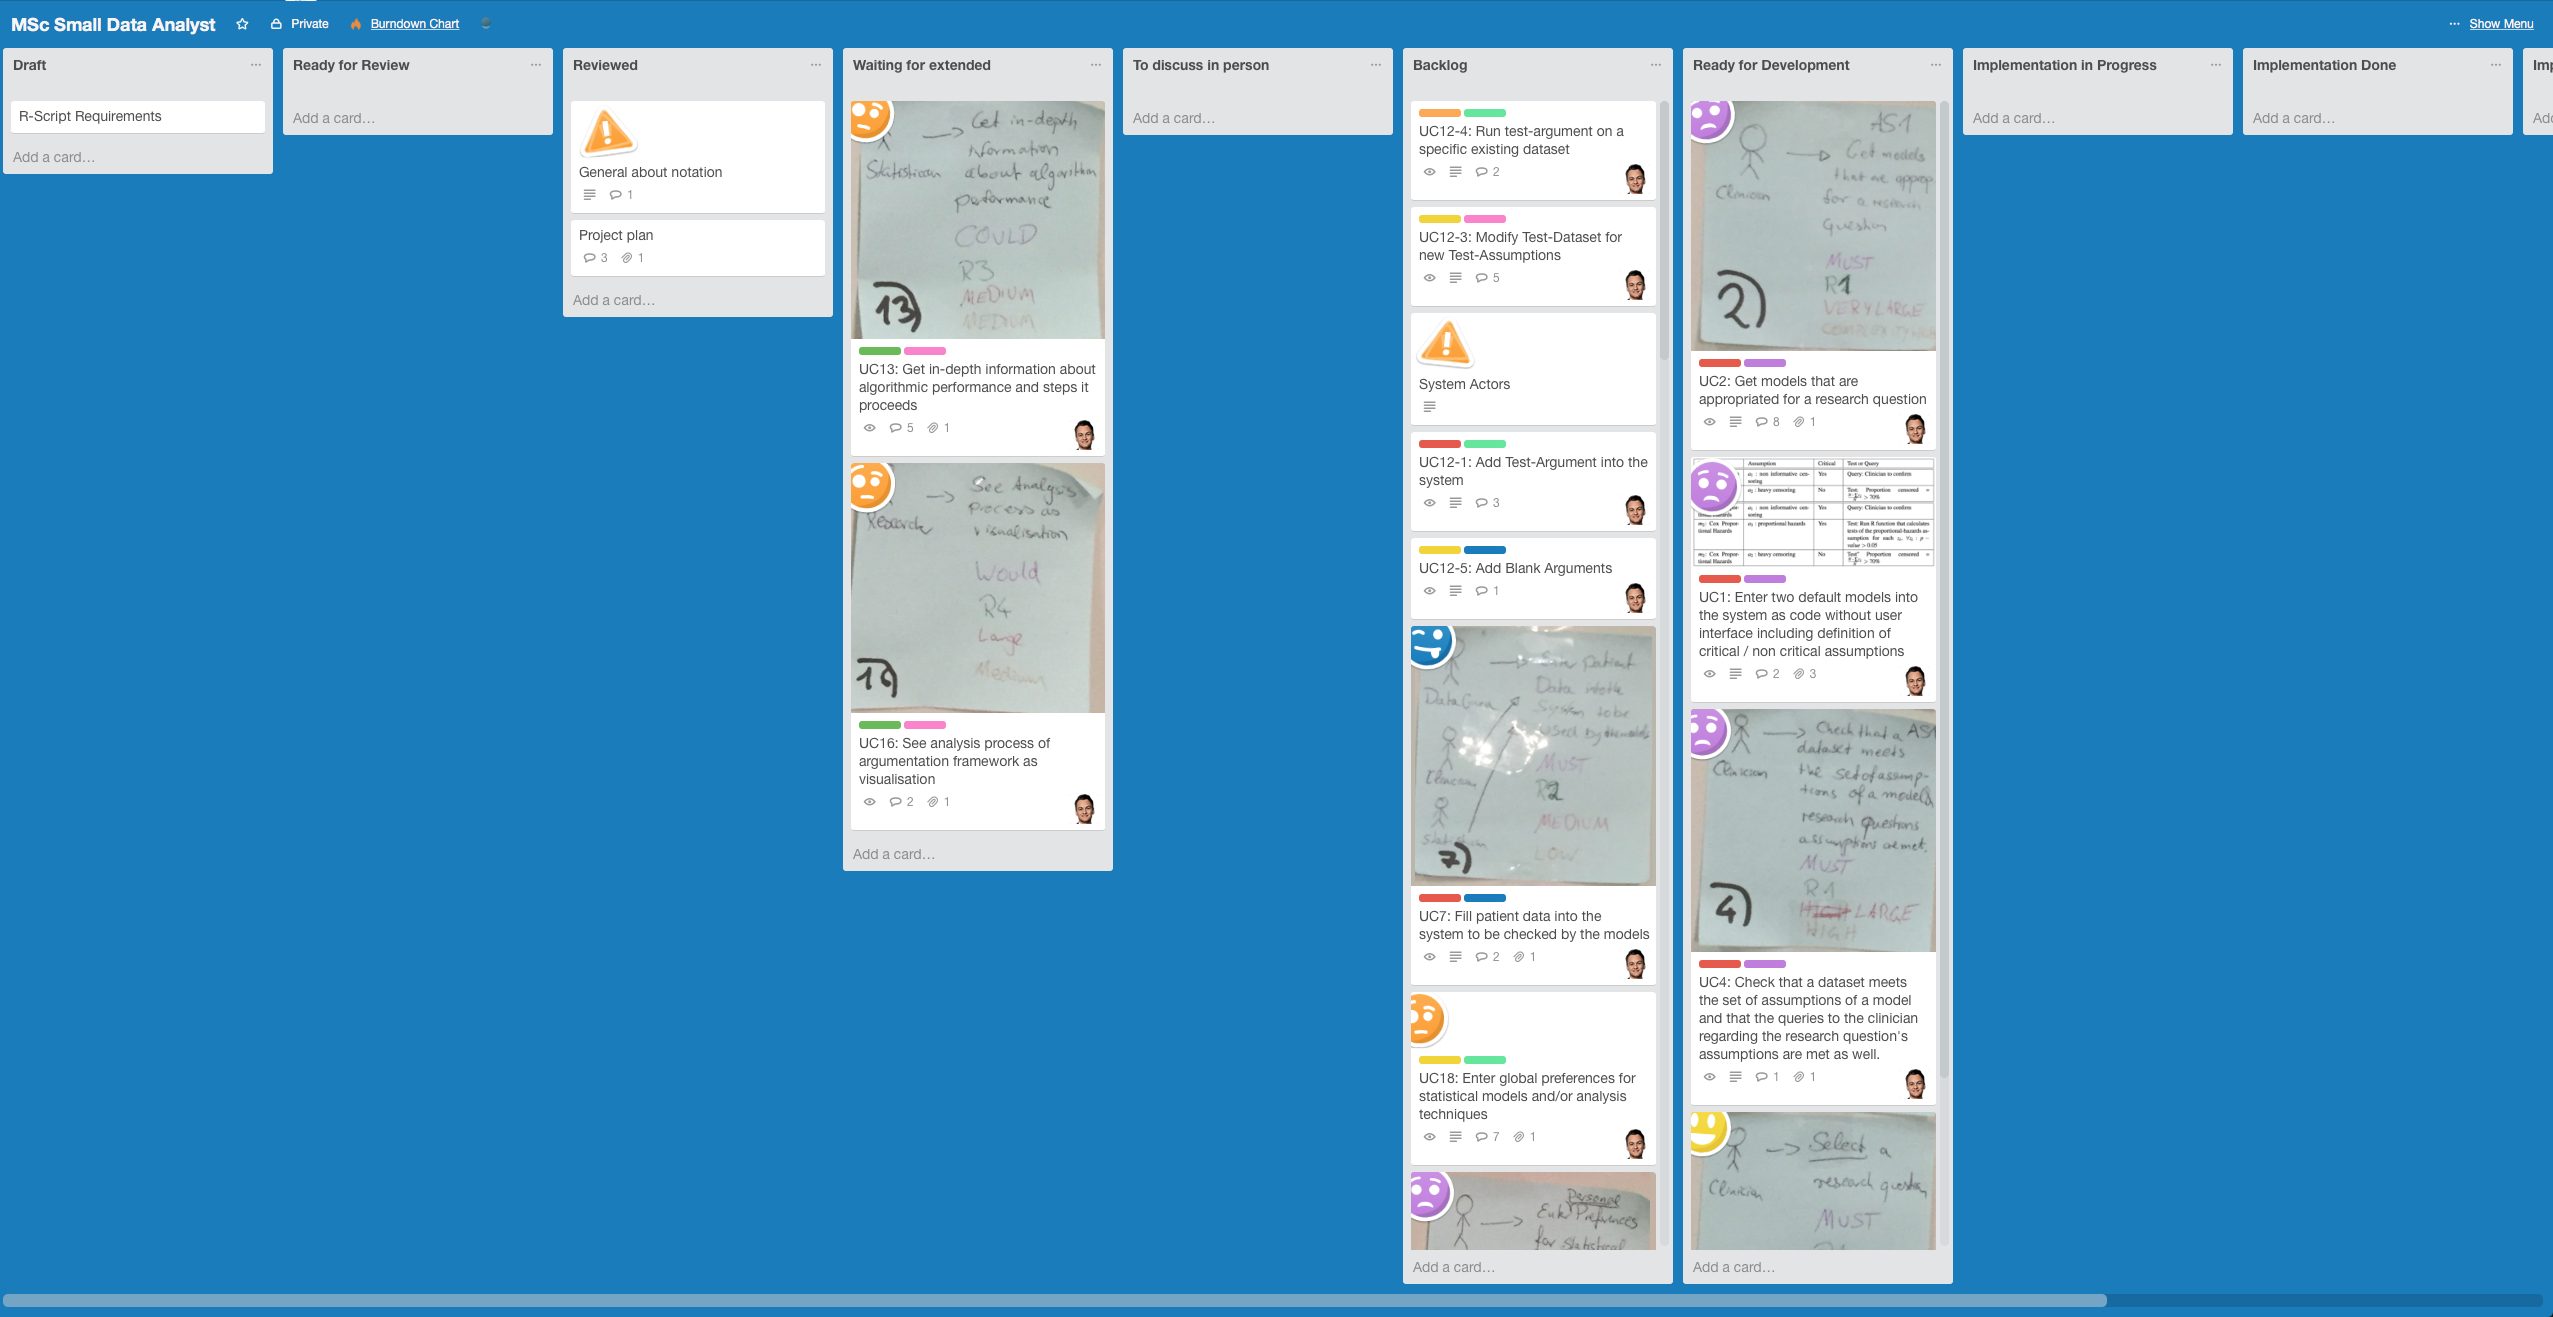
\includegraphics[page=1,width=\textwidth]{figures/trello}
\caption{Screenshot of the used Trello board used as project management tool}
\label{fig:trello}
\end{figure}

\subsection{Supplementary Resources}

During this Masters Project a web-application has been developed which is public available on \href{http://small-data-analyst.herokuapp.com}{http://small-data-analyst.herokuapp.com}. Users can sign-up (needs approval of an administrator, please reach out to the author if you have any questions related to that) and upload there own datasets. Some of the existing research question are public available and shared between all users of the application. However -- if required -- the source code is available on \href{https://github.com/sebastianzillessen/small-data-analyst}{Github}\footnote{\href{https://github.com/sebastianzillessen/small-data-analyst}{https://github.com/sebastianzillessen/small-data-analyst}} and a installation instruction can be found in the appendix \autoref{app:installation}. A detailed list of used third-party applications can be found in \autoref{app:3rdparty}.


\section{Background Research}
\label{sec:background}

A lot of medical data is collected nowadays on a routine basis by clinicians and could play a critical role to support evidence based decision-making. However, the process of analysing the data and selecting the "correct" statistical model is often a demanding process for clinicians. A system helping them to select and apply appropriate models on these clinical data sets would empower them -- even with minimal or no statistical knowledge -- to make data driven decisions. 

It has been shown in \cite{sassoon2014}, that a system based on argumentation schemes and a statistical knowledge base could close the gap between the clinician performing analysis and the statistician having the in-depth knowledge of the underlying theory. The relevant theoretical elements will be explained in the following sections.


\subsection{Structure of the Background Research}

The approach for a statistical model selection proposed in \cite{sassoon2014} is based on computational models of argumentation. Usually multiple assumptions have to be fulfilled for statistical models to be applicable on a data set. These assumptions are defeasible and may lead to multiple possible models, which requires argumentation over assumptions and models to provide a reasonable statistical model selection. An introduction to \glspl{AF} is given in \autoref{sub:dung}. 

Non-monotonic argumentation (as proposed in \cite{dung1995,liao}) and monotonic (classic) logic (as proposed in \cite{Reiter1980}) are in general different approaches to deal with reasoning. However, recent research is focusing on dialogue based approaches, which are mostly based on non-monotonic argumentation \cite{parsons2000,Walton1995}. 
Nevertheless Sassoon \textit{et al.} propose to employ preferences by using \glspl{EAF} to reason about the order of applicable models and to deliver a final statistical model that should be used. 

To understand this approach, an extension to the standard framework to reason over preferences is presented later in this section (see \autoref{sub:eaf}). Other possible solutions to argue over preferences are explained in \autoref{sub:paf}.

Finally, \autoref{sub:statistical_model_selection} provides a summary of Sassoon \textit{et al.} \cite{sassoon2014} on the problem of finding applicable and choosing preferred models by clinicians for a given research question. In our application we focused on the approach described by the most recent papers \cite{sassoon2016,sassoon2016CD}, which will be summarised as well.


\subsection{Argumentation Theory: General introduction}
\label{sub:dung}
In the following section a general overview on \glspl{AF} will be given. The notation and definitions are based on Dung's theory \cite{dung1995} as it is a widely used definition for argumentation frameworks and the main sources of this dissertation \cite{sassoon2014,sassoon2016CD,Modgil2009} are based on this approach.
\begin{definition}
	An argumentation framework is a tuple $AF = \langle \S, \R \rangle$ where $\S$ is a set of arguments and $ \R \subseteq \S \times \S$. $\R$ is a binary relation and called attack relation.
\end{definition}


An (abstract) argumentation framework can be represented as a directed graph where nodes are arguments and an arrow from a node $A$ to a node $B$ represents an attack from argument $A$ against $B$.

\begin{remark}
	Later in this dissertation assumptions that need to hold for a specific model are introduced. They are as well represented as a directed graph, but here an edge from assumption $A$ to model $B$ denotes that the assumption $A$ needs to hold so that $B$ is a possible model. However, the difference will be determinable from the context.
\end{remark}


\begin{exa}
 \autoref{fig:small_af} represents an \gls{AF} with the definition $AF = \langle \{A, B, C, D, E\}, \allowbreak \{(A,B), (B, C),\allowbreak (B, E), (C, B),\allowbreak (D,C), (D,D)\} \rangle $. This framework will be used as an example for the following definitions.
\end{exa}


\begin{figure}[h]
\centering
\begin{tikzpicture}[->,>=stealth',shorten >=1pt,auto,node distance=2cm,
                    thick]

  \node[main ] (A) {A};
  \node[main ] (B) [right of=A] {B};
  \node[main ] (C) [right of=B] {C};
  \node[main ] (D) [below of=C] {D};
  \node[main ] (E) [below of=B] {E};
  
  \path[every node/.style={font=\sffamily\small}]
    (A) edge node [left] {} (B)
    (B) edge [bend right] node [left] {} (C)
    	edge node [left] {} (E)
    (C) edge [bend right] node [left] {} (B)
    (D) edge node [left] {} (C)
        edge [loop right] node {} (D)
    ;
\end{tikzpicture}
\caption{Small example argumentation framework.}
\label{fig:small_af}
\end{figure}


\begin{notation}
In this paper we use capital letters $\{A, B, ...\}$ to denote arguments. $AB$ or $(A, B)$ denotes an attack from $A$ to $B$ ($(A,B) \in \R$).	
\end{notation}

For the following definitions let $AF=\langle \S, \R \rangle, S' \subseteq \S$.

\begin{definition}
	A subset $S'$ is \textbf{conflict-free} iff $ \forall A, B \in S': (A, B) \notin \R$ \textit{(the subset has no attacks between its arguments)}.
\end{definition}
\begin{remark}
	Conflict-free subsets are of interest, as these sets are not directly contradictory. In other words, a conflict-free subset of an argumentation framework does not contain any attacks between its members.
\end{remark}
\begin{exa}
Conflict-free subsets in the provided example are $\emptyset, \{A\}, \{B\}, \{C, E\}, ...$. The sets $\{D\}, \{A, B\}, \{B, C\}$ are not conflict-free.
\end{exa}

\begin{definition}
$A$ is \textbf{acceptable} w.r.t. a subset $S'$ iff  $\forall B \in \S: (B, A) \in \R \Rightarrow \exists C \in S': (C, B) \in \R$ \textit{(an argument $A$ is acceptable with respect to a subset $S'$ iff for each attacker $C$ of $A$ there is an argument in $S'$ that attacks this attacker of $A$). }
\end{definition}

\begin{remark}
If an argument $A$ is acceptable w.r.t. a subset $S'$, then there exists no holding counter-argument in this \gls{AF} causing the argument $A$ not to hold.
\end{remark}

\begin{lemma}
	$S'$ \textbf{defends} $X$, if and only if $X$ is acceptable with respect to $S'$.
\end{lemma}

\begin{exa}
In  \autoref{fig:small_af} $E$ is acceptable with respect to $\{A\}$. $A$ is acceptable with respect to $\emptyset$. 
\end{exa}


\begin{definition}
The \textbf{characteristic function} of an argumentation framework $AF$ (denoted as $F_{AF}$) is defined by the following:
	\begin{align*}
		&F_{AF}: 2^{\S} \rightarrow 2^\S &\\
		&F_{AF}(S') = \{A | A~\text{is acceptable with respect to}~S'\} &
	\end{align*}
\end{definition}
\begin{notation}
	If it is unambiguous, we often refer to $F_{AF}$ with $F$. 
\end{notation}

\begin{definition}
	A conflict-free set $S' \subseteq \S$ is \textbf{admissible} iff $S'$ defends all of its arguments (\textit{each argument in $S'$ is acceptable with respect to $S'$}) or $S' \subseteq F_{AF}(S')$.
\end{definition}

\begin{exa}
In the given example in \autoref{fig:small_af} sets $\{A\}, \{A, E\}$ are admissible, and $\{B\}$ is conflict-free but not admissible, since $B$ is not acceptable with respect to $\{B\}$.
\end{exa}

\begin{definition}
$S'$ is a \textbf{complete extension} iff  $S'$ is admissible and each argument that is acceptable with respect to $S'$ (which is defended by $S'$) belongs to $S'$.
\end{definition}

\begin{remark}
	A complete extension is a set of arguments that defends all members and includes all arguments that can be accepted regarding these members. In \autoref{fig:small_af} the set $S'=\{A\}$ is acceptable, but as this set defends as well $E$ (the only attacker $B$ is not acceptable w.r.t. $S'$), this argument must be included in $S'$ to make the set complete. Hence $S' = \{A, E\}$ is a complete extension. 
\end{remark}


\begin{exa}
$X = \{A, E\}$ is a complete extension in \autoref{fig:small_af}, since it is admissible and it defends $A$ and $E$. Note that $C$ is not defended by $X$ since it does not attack $D$ and $D$ cannot be defended.
Complete extensions in \autoref{fig:pref_af} are $\{A\}, \{A, C\}$ and $\{A, D\}$.
\end{exa}


\begin{definition}
A grounded extension ($GE_{AF}$) of an argumentation framework $AF$ is the minimal (with respect to set inclusion) complete extension of $AF$. In other words $GE_{AF}$ is the least fixed point of $F_{AF}$. ($GE_{AF} = F_{AF}(\emptyset)$).
\end{definition}

\begin{remark}
	The grounded extension can be understood as the set of arguments an rational agent can accept without doubts, as it contains only the minimal acceptable arguments for an argumentation framework and does not require the agent to assume anything about any argument.
\end{remark}

\begin{exa}
	The grounded extension of the example framework in \autoref{fig:small_af} is $\{A, E\}$.
	The grounded extension of the example framework in \autoref{fig:pref_af} is $\{A\}$.
\end{exa}


\begin{definition}
\label{def:preferred_extension}
A preferred extension of an argumentation framework $AF$ is a maximised (with respect to set inclusion) admissible set of $AF$.
\end{definition}

\begin{figure}[t]
\centering
\begin{tikzpicture}[->,>=stealth',shorten >=1pt,auto,node distance=2cm,
                    thick]

  \node[main] (A) {A};
  \node[main] (B) [right of=A] {B};
  \node[main] (C) [right of=B] {C};
  \node[main] (D) [right of=C] {D};
  \node[main] (E) [right of=D] {E};
  
  \path[every node/.style={font=\sffamily\small}]
    (A) edge node [left] {} (B)
    (C) edge node [left] {} (B)
    	edge [bend right] node [left] {} (D)
    (D) edge [bend right] node [left] {} (C)
	    edge [] node [left] {} (E)
    (E) edge [loop right] node {} (E)
    ;
\end{tikzpicture}
\caption{Argumentation framework used for some examples. }
\label{fig:pref_af}
\end{figure}

\begin{exa}
The preferred extensions in \autoref{fig:pref_af} are $\{A, C\}$ and $\{A, D\}$.
\end{exa}

\begin{definition}
A conflict-free set of arguments $S' \subseteq \S$ is called a \textbf{stable extension} iff $S'$ directly attacks each argument which does not belong to $S'$.
\end{definition}
\begin{exa}
The $AF$ in \autoref{fig:pref_af} has the stable extension $\{A, D\}$. $\{A, C\}$ is a preferred, but not a stable extension.
\end{exa}


\begin{remark}
The different extensions of a $AF = \langle \S, \R \rangle$ have the following relations between each other \cite{dung1995}:
\begin{itemize} 
	\item Each preferred extension is as well a complete extension.
	\item Each stable extension is as well a preferred extension.
	\item The grounded extension is the least (with respect to set inclusion) complete extension and therefore unique for each $AF$.
	\item Preferred extensions are the most (with respect to set inclusion) complete extensions.
	\item Arguments accepted in the grounded extension are skeptically accepted in the $AF$.
	\item Every $AF$ has at least one preferred extension.
	\item A stable extension does not always exist.
\end{itemize}
\end{remark}


\begin{definition}	
	An argument is regarded as \textbf{sceptically accepted under a semantic}, iff it is accepted in all extensions of this semantic (complete, grounded, preferred, stable). An argument is regarded as \textbf{credulously accepted under a semantic}, iff it accepted in at least one, but not all, extensions of this semantic. 	
\end{definition}

\begin{exa}
	In \autoref{fig:pref_af} $\{A\}$ is sceptically accepted under each semantic. $\{C, D\}$ are credulously accepted under a preferred semantic. $\{D\}$ is as well accepted sceptically under the stable semantic.
\end{exa}


Furthermore \cite{dung1995} introduces \textit{well-founded argumentation frameworks} (having exactly one extension which is grounded, preferred and stable), \textit{uncontroversial argumentation frameworks} and \textit{coherent argumentation frameworks} (each preferred extension of an $AF$ is stable). Regarding the problem we are looking at, defeasible argumentation is really important, as we are dealing with inconsistent \glspl{SKB}. Hence these restricted argumentation frameworks will not be used in this project, therefore they are not discussed any further.


In addition to the discussed extension-based semantics, \cite{liao} introduces a so called \textit{labelling-based approach} where there are usually three labels: \texttt{IN} (accepted argument), \texttt{OUT} (rejected argument) and \texttt{UNDEC} (undecided whether this argument is accepted or rejected) and a labelling function $\lambda: \S \rightarrow \{IN, OUT, UNDEC\}$.

By defining legally labelled arguments, definitions for \textit{conflict-free labelings},~\textit{admissible labelings} and \textit{complete/grounded/preferred labelings} can be derived. As there exists a bijective projection, they can be easily transferred to the extension-based semantics already introduced in this section. This labelling based approach has been used to implement the solving algorithm described in \cite{Modgil2009Labellings} later in this thesis (see \autoref{sub:eaf_algorithm}).



\newacronym{EAF}{EAF}{Extended argumentation framework}
\glsreset{EAF}
\subsection{\gls{EAF} - Working with Preferences in $AF$}

A Dung's argumentation framework is based on logical theory which is transformed to arguments and a binary attack relation. By applying the different extensions on the created argumentation framework accepted arguments can be evaluated. \todo{"This approach does not consider, that for practical reasons and in some applications only one unique set of accepted arguments has to be determined, where personal preferences, contextual requirements or additional information might result in some arguments having a higher priority compared to others.": ok, but this sentence is quite long.  Consider splitting it.
}This approach does not consider, that for practical reasons and in some applications only one unique set of accepted arguments has to be determined, where personal preferences, contextual requirements or additional information might result in some arguments having a higher priority compared to others. This order of preferences is often itself defeasible and conflicting and therefore subject to argumentation \cite{Modgil2009}.



In this thesis the \gls{EAF} approach introduced by Modgil in \cite{Modgil2009} will be used, as it provides a useful meta-level on preferences between other arguments, by extending Dung's framework with a new attack relation between arguments and attacks. This overcomes the issues of defining orders over preferences (see \autoref{sub:paf}) or value-evaluation functions (see \autoref{sub:vaf}) and enables us to argue about preferences regardless whether they are defeasible or conflicting. In addition it provides a really user-friendly way to consider preferences which will improve the understandability for clinicians, who will be the main actors (see \autoref{sub:sassoon:actors}) in the final system.
\autoref{fig:eaf_intro}, which is taken from \cite{Modgil2009}, shows an example for a \gls{EAF} representing the following arguments:

\begin{itemize}
	\item $A$: "Today will be dry in London since the BBC forecast sunshine"
	\item $B$: "Today will be wet in London since CNN forecast rain"
	\item $C$: "But I think the BBC are more trustworthy than CNN"
	\item $D$: "However, statistically CNN are more accurate forecasters than the BBC"
	\item $E$: "Basing on a comparison on statistics is more rigorous and rational than basing a comparison on your instincts about their relative trustworthiness"
\end{itemize}

\begin{figure}[b!]
\centering
\begin{tikzpicture}[->,>=stealth',shorten >=1pt,auto,node distance=2cm,
                    thick]

  \node[main node] (A) {A};
  \node[small,n_fill_green] (B) [left of=A] {B};
  \node[small,n_fill_green] (C) [above right of=A] {C};
  \node[main node] (D) [below right of=A] {D};
  \node[small,n_fill_green] (E) [right=3cm of A] {E};
  
  \path[every node/.style={font=\sffamily\small}]
    (A) edge [bend right, dashed] coordinate [pos=0.5] (AB) node [left] {} (B)
    (B) edge [bend right] coordinate [pos=0.5] (BA) node [left] {} (A)
    (C) edge [bend right] coordinate [pos=0.5] (CD) node [left] {} (D)
    (D) edge [bend right, dashed] coordinate [pos=0.5] (DC) node [left] {} (C)
    ;
   \path [every node/.style={red}] 
   (C) edge [->>, bend right] node [left] {} (AB)
   (D) edge [->>, bend left, dashed] node [left] {} (BA)
   (E) edge [->>] node [left] {} (DC)
   ;
\end{tikzpicture}
\caption{\gls{EAF} about the weather forcasts with preferences over arguments. Dashed attacks are canceled out. Double-arrow-headed edges represent attacks on attacks. Green nodes represent accepted arguments in the unique preferred extension.}
\label{fig:eaf_intro}
\end{figure}


\glsreset{EAF}
\begin{definition}
\todo{Definition 2.15: State more explicitly in your definition that this relationship consists of attacks by arguments on other attacks.}
	An \gls{EAF} is a triple $\langle \S, \R, \D \rangle$ with $\S$ being a set of arguments and:
	\begin{itemize}
		\item $\R \subseteq \S \times \S$: attack relation.
		\item $\D \subseteq \S \times \R$: new attack relation on attacks.
		\item $\{(A, (B, C)), (A', (C, B))\} \subseteq \D \rightarrow \{(A, A'), (A', A)\} \subseteq \R$ (any arguments expressing contradictory preferences must attack each other).
	\end{itemize}
\end{definition}

\begin{remark}
\todo{Remark 2.16: OK, but it would be better to state this in your own words rather than use a quote.}
"If $A$ attacks $(B, C) \in \R$ then $A$ expresses, that $C$ is preferred to $B$. If $A'$ attacks $(C, B)$, then $A'$ expresses that $B$ is preferred to $C$. Hence \glspl{EAF} are required to conform to the constraint that any such arguments expressing contradictory preferences must attack each other."\cite{Modgil2009}.
\end{remark}

Let $\Delta = \langle \S, \R, \D \rangle$ be a \gls{EAF} and $S' \subseteq \S$ for the following definitions.

\begin{definition}
$A$ \textbf{defeats$_{S'}$} $B$ iff $(A, B) \in \R$ and $\not \exists C \in S': (C, (A, B)) \in \D$. If $A$ defeats\low{S'} $B$ and $B$ does not defeat\low{S'} $A$ then $A$ \textbf{strictly} defeats\low{S'} $B$.
\end{definition}

\begin{notation}
For the rest of the document $A \rightarrow^{S'} B$ denotes that $A$ defeats\low{S'} B and $A \nrightarrow^{S'} B$ denotes that $A$ does not defeat\low{S'} $B$.
\end{notation}


By using this definition, similar properties (e.g. conflict-free and admissible sets, acceptability of an argument, sceptically/credulously accepted arguments, extensions) as in Dung's argumentation framework can be introduced and defined.

\begin{definition}
	$S'$ is \textbf{conflict free} iff $\forall A, B \in S': (A, B) \in \R \Rightarrow (B, A) \notin \R \wedge \exists C \in S': (C, (A, B)) \in \D$ \textit{(a subset is only conflict free, if for every attack within the subset there is no counter attack and the attack itself is canceled out by an attack on this attack from an argument that is part of the subset as well)}.
\end{definition}


\begin{figure}[h]
\centering
\begin{tikzpicture}[->,>=stealth',shorten >=1pt,auto,node distance=2cm,
                    thick]

  \node[main node] (C) [above right of=A] {C};
  \node[main node] (A) [below left of=C]{A};
  \node[main node] (B) [below right of=C] {B};
  
  \path[every node/.style={font=\sffamily\small}]
    (A) edge [] coordinate [pos=0.5] (AB) node [left] {} (B)
    ;
   \path [every node/.style={red}] 
   (C) edge [->>] node [left] {} (AB)
   ;
\end{tikzpicture}
\caption{\gls{EAF} with $\langle \S, \R, \D \rangle = \langle \{A, B, C\}, \{(A, B)\}, \{(C, (A, B))\} \rangle$.}
\label{fig:eaf_small}
\end{figure}

\begin{exa}
	The set $S' = \{A, B\}$ of the \gls{EAF} in \autoref{fig:eaf_small} is not conflict-free. But the set $S' = \{A, B, C\}$ is conflict-free as $C$ attacks the attack between $A$ and $B$ and cancels it out.
\end{exa}

\begin{lemma}
Let $S'$ be a conflict-free subset of $\S$ in $\langle \S, \R, \D \rangle$. Then for any $A, B \in S'$ $A$ does not defeat\low{S'} $B$.
\end{lemma}

\begin{definition}
\todo{Definition 2.21: Add an intuitive explanation of what a "reinstatement set" is.
You should explain how the concepts discussed in 2.2 apply to your work!}
$R_{S'} = \{X_1 \rightarrow^{S'} Y_1, ..., 	X_n \rightarrow^{S'} Y_n\}$ is called a \textbf{reinstatement set} for $C \rightarrow^{S'} B$ ($C$ defeats\low{S'} $B$), iff:
\begin{itemize}
	\item $C \rightarrow^{S'} B \in R_{S'}$,
	\item $\forall_{i=1}^n X_i \in S'$,
	\item $\forall X \rightarrow^{S'} Y \in R_{S'}, \forall Y': (Y', (X, Y)) \in \D$, there is a $X' \rightarrow^{S'} Y' \in R_{S'}$.
\end{itemize}
\end{definition}

The acceptability of an argument can now be formally defined based on the reinstatement set.

\begin{definition}
$A \in \S$ is \textbf{acceptable} w.r.t.	 $S'$, iff: $\forall B: B \rightarrow^{S'} A$, there is a $C \in S': C \rightarrow^{S'} B$ and there is a reinstatement set for $C \rightarrow^{S'} B$.
\end{definition}


\begin{figure}[h]
	\centering
	\subfigure[0.3\textwidth][$A_1$ is not acceptable w.r.t $S' = \{A_1, A_2\}$]{
		\begin{tikzpicture}[->,>=stealth',shorten >=1pt,auto,node distance=1.2cm,thin]
		
		  \node[n_fill_red,small] (A1) [] {$A_1$};
		  \node[n_fill_gray,small] (A2) [right of=A1]{$A_2$};
		  \node[small] (B1) [below of=A1] {$B_1$};
		  \node[small] (B2) [below of=A2] {$B_2$};
		  \node[small] (B3) [right of=B2] {$B_3$};
		      
		  \path[every node/.style={font=\sffamily\small}]
		    (A1) edge [bend left] coordinate [pos=0.5] (A1B1) node [left] {} (B1)
		    (B1) edge [bend left] coordinate [pos=0.5] (B1A1) node [left] {} (A1)
			(A2) edge [] coordinate [pos=0.5] (A2B2) node [left] {} (B2)
		    ;
		   \path [every node/.style={red}] 
		   (B2) edge [->>] node [left] {} (A1B1)
		   (B3) edge [->>] node [left] {} (A2B2)
		   ;
		\end{tikzpicture}
		\label{fig:eaf_not_acceptable}
	}
	\hfill
	\subfigure[0.3\textwidth][$C$ is acceptable w.r.t $S' = \{A_1, A_2, A_3\}$]{
		\begin{tikzpicture}[->,>=stealth',shorten >=1pt,auto,node distance=1.2cm,
		                    thin]
		
		  \node[n_fill_gray,small] (A1) [] {$A_1$};
		  \node[n_fill_gray,small] (A2) [right of=A1]{$A_2$};
		  \node[n_fill_gray,small] (A3) [right of=A2]{$A_3$};
		  \node[small] (B1) [below of=A1] {$B_1$};
		  \node[small] (B2) [below of=A2] {$B_2$};
		  \node[small] (B3) [below of=A3] {$B_3$};
		  \node[n_fill_green,small] (C) [left of=B1] {$C$};      
		
		  \path[every node/.style={font=\sffamily\small}]
		    (A1) edge [] coordinate [pos=0.5] (A1B1) node [left] {} (B1)
		    (A2) edge [] coordinate [pos=0.5] (A2B2) node [left] {} (B2)
		    (A3) edge [] coordinate [pos=0.5] (A3B3) node [left] {} (B3)
			(A2) edge [] coordinate [pos=0.5] (A2B2) node [left] {} (B2)
			(B1) edge [] coordinate [pos=0.5] (B1C) node [left] {} (C)
		    ;
		   \path [every node/.style={red}] 
		   (B2) edge [->>] node [left] {} (A1B1)
		   (B2) edge [->>] node [left] {} (A3B3)
		   (B3) edge [->>] node [left] {} (A2B2)
		   ;
		\end{tikzpicture}
		\label{fig:eaf_acceptable}
	}
	\hfill
	\subfigure[0.3\textwidth][$C$ is not acceptable w.r.t $S' = \{A_1, A_2, A_3\}$]{
		\begin{tikzpicture}[->,>=stealth',shorten >=1pt,auto,node distance=1.2cm,
		                    thin]
		
		  \node[n_fill_gray,small] (A1) [] {$A_1$};
		  \node[n_fill_gray,small] (A2) [right of=A1]{$A_2$};
		  \node[n_fill_gray,small] (A3) [right of=A2]{$A_3$};
		  \node[small] (B1) [below of=A1] {$B_1$};
		  \node[small] (B2) [below of=A2] {$B_2$};
		  \node[small] (B3) [below of=A3] {$B_3$};
		  \node[small] (B4) [right of=B3] {$B_4$};
		  \node[n_fill_red,small] (C) [left of=B1] {$C$};      
		
		  \path[every node/.style={font=\sffamily\small}]
		    (A1) edge [] coordinate [pos=0.5] (A1B1) node [left] {} (B1)
		    (A2) edge [] coordinate [pos=0.5] (A2B2) node [left] {} (B2)
		    (A3) edge [] coordinate [pos=0.5] (A3B3) node [left] {} (B3)
			(A2) edge [] coordinate [pos=0.5] (A2B2) node [left] {} (B2)
			(B1) edge [] coordinate [pos=0.5] (B1C) node [left] {} (C)
		    ;
		   \path [every node/.style={red}] 
		   (B2) edge [->>] node [left] {} (A1B1)
		   (B2) edge [->>] node [left] {} (A3B3)
		   (B3) edge [->>] node [left] {} (A2B2)
		   (B4) edge [->>] node [left] {} (A3B3)
		   ;
		\end{tikzpicture}
		\label{fig:eaf_not_acceptable_big}
	}
	\caption{\glspl{EAF} with acceptable and not acceptable sets $S'$. $A_x$ are elements of $S'$.}
\end{figure}

\begin{exa}
	In Figure \autoref{fig:eaf_not_acceptable} $S'=\{A_1, A_2\}$ is not admissible since $A_1$ is not acceptable w.r.t. $S'$. In Figure \autoref{fig:eaf_acceptable} $C$ is acceptable w.r.t $S' = \{A_1, A_2, A_3\}$ as there is a reinstatement set $\{A_1 \rightarrow^{S'} B_1, A_2 \rightarrow^{S'} B_2, A_3 \rightarrow^{S'} B_3\}$ for $A_1 \rightarrow^{S'} B_1$. In Figure \autoref{fig:eaf_not_acceptable_big} there is an additional argument $B_4$ such that $B_4 \rightarrow (C_3 \rightarrow B_3)$ and no argument in $S'$ that defeats\low{S'} $B_4$, then no reinstatement set for $A_1 \rightarrow^{S'} B_1$ would exist, hence $C$ is not acceptable w.r.t. $S'$.
\end{exa}

Similar to Dung's theory, admissible, preferred, complete and stable extensions of an \gls{EAF} can now be defined.


\begin{definition}
	Let $S'$ be a \textbf{conflict free} subset of $\S$ in $\langle \S, \R, \D \rangle$. Then:
	\begin{itemize}
		\item $S'$ is an \textbf{admissible} extension iff every argument in $S'$ is acceptable w.r.t $S'$.
		\item $S'$ is a \textbf{preferred} extension iff $S'$ is (w.r.t. set inclusion) a maximal admissible extension.
		\item $S'$ is a \textbf{complete} extension iff each argument which is acceptable w.r.t. $S'$ is in $S'$.
		\item $S'$ is a \textbf{stable} extension iff $\forall B \notin S', \exists A \in S'$ such that $A$ defeats\low{S'} $B$.
	\end{itemize}
\end{definition}


By using this definition, we can define again \textbf{sceptically}, respectively \textbf{credulously}, accepted arguments under the semantic $ s \in $\{preferred, complete, stable\} iff $A$ is in every (at least one) $s$ extension. 
\begin{exa}
	The example given in \autoref{fig:eaf_intro} has only the single preferred, complete and stable extension $\{B, C, E\}$. \autoref{fig:eaf_small} has the admissible sets $\{A\}, \{A, C\}, \{A, B, C\}$. $\{A, B, C\}$ is the only preferred extension which is as well stable.
\end{exa}

\begin{lemma}
	Let $\Delta = \langle \S, \R, \D \rangle$ be an \gls{EAF}, $S'$ an admissible extension of $\Delta$ and let $A, A'$ be arguments which are acceptable w.r.t. $S'$. Then:
	\begin{itemize}
		\item $S'' = S' \cup \{A\}$ is admissible.
		\item $A'$ is acceptable w.r.t. $S''$.
	\end{itemize}	
\end{lemma}

\begin{lemma}
	Let $\Delta = \langle \S, \R, \D \rangle$ be an \gls{EAF}. 
	\begin{itemize}
		\item The set of all admissible extensions of $\Delta$ form a complete partial order w.r.t. set inclusion.
		\item For each admissible extension $E$ of $\Delta$ there exists a preferred extension $E'$ such that $E\subseteq E'$.
	\end{itemize}
	\label{lem:eaf:partialorder}
\end{lemma}

The definition of the characteristic function for an \gls{EAF} is similar but not equal to Dung's definition. 

\begin{definition}
	Let $\Delta = \langle \S, \R, \D \rangle$ be an \gls{EAF}, $S'\subseteq \S$, and $2^{\S_C}$ denote the set of all conflict free subsets of $\S$. The \textbf{characteristic function} $F_\Delta$ of $\Delta$ is defined as follows:
	\begin{itemize}
		\item $F_\Delta: 2^{\S_C} \rightarrow 2^{\S}$
		\item $F_\Delta(S') = \{A | A~\text{is acceptable w.r.t.~}S'\}$.
	\end{itemize}
\end{definition}

From here on we will always refer to a fixed \gls{EAF}, hence we can simply write $F$ rather than $F_\Delta$. Equally to Dung's Framework, any conflict-free set $S' \subseteq \S$ in $\Delta$ is admissible iff $S' \subseteq F(S')$, and complete iff $S'$ is a fixed point of $F$. We can apply $F$ iteratively on an \gls{EAF}: $F^0 = \emptyset, F^{i+1} = F(F^i))$. Note, that for \glspl{EAF} the characteristic function $F$ is in general \textbf{not} monotonic (e.g. $C$ is acceptable w.r.t $S'= \{A_1, A_2, A_3\}$ in \autoref{fig:eaf_acceptable}, but is not acceptable w.r.t. the conflict-free $S'' = S' \cup \{B_2, B_3\}$).
\begin{lemma}
Let $F$ be the characteristic function of an \gls{EAF}, and $F^0 = \emptyset, F^{i+1} = F(F^i)$. Then $\forall i, F^i \subseteq F^{i+1}$ and $F^i$ is conflict free.
\end{lemma}


\begin{definition}
	$\Delta = \langle \S, \R, \D \rangle$ is a \textbf{finitary} \gls{EAF} iff $\forall A \in \S$, the set $\{B | (B, A) \in \R\}$ is finite and $\forall (A, B) \in \R$, the set $\{C | (C, (A, B))\in \D\}$ is finite.
\end{definition}

\begin{definition}
	Let $\Delta$ be a finitary \gls{EAF} and $F^0 = \emptyset, F^{i+1} = F(F^i)$. Then $\cup_{i=0}^\infty(F^i)$ is the \textbf{grounded extension} $GE(\Delta)$ of $\Delta$.
\end{definition}


\begin{remark}
Similar to Dung's framework we can state the following relations between different extensions:
\begin{itemize}
	\item Every \gls{EAF} has at least one preferred extension (implied by \autoref{lem:eaf:partialorder} as $\emptyset$ is an admissible extension for every \gls{EAF}).
	\item Every stable extension of an \gls{EAF} is a preferred extension.
	\item The grounded extension for \gls{EAF} is not defined over the least fix point of the characteristic function $F$, but can be defined for finitary \glspl{EAF} over the union of all characteristic functions $F^i$.
\end{itemize}	
\end{remark}

In addition Modgil \textit{et al.} introduce in \cite{Modgil2009} the concept of a special class of \glspl{EAF}, \textit{hiearchical \glspl{EAF}}, which are defined by the existence of a partition of $\Delta$ into multiple regular Dung argumentation frameworks. Due to this restriction it is possible to define a least fix point of the characteristic function $F$, hence defining the grounded extension $GE(\Delta)$ in the same way as it has been defined in Dung's framework.

Furthermore \cite{Modgil2009} presents as well the concept of \textbf{Preference symmetric extended argumentation frameworks}. This extension limits the attacks on attacks (so the set $\D$) only on attacks between symmetrically attacking arguments. However, this is a to narrow restriction for our purposes, therefore this will not be described here. 




A short overview over other approaches to deal with preferences in argumentation frameworks can be found in \autoref{app:other_afs}. 
\subsection{Related source paper}
The foundation of this MSc Project is the paper \cite{sassoon2014}. The goal of this project is to use Argumentation Theory for Statistical Model Selection in mostly clinical environments. The increasing availability and the growing size of datasets available for clinicians and the raising awareness on evidence based decision making extend the demand into systems that support clinicians in the analysis of this data in their day-to-day practice. In the following section a short summary on the paper will be given. More details can be found in the following parts of the paper.

To overcome the issue of clinicians analysing data and models on there compatibility \cite{sassoon2014} proposes an approach of an intelligent model selection system which is capable of suggesting appropriate model(s) to a clinician during the design stage of a study, taking in account the research question, the clinical data and any external relevant input and preferences. In addition this system should be able of supporting its decision by providing the argumentation for and against a model to the user. As clinicians might not always be qualified to perform the statistical analysis required for their research question, the process of designing models, specifying its requirements and providing the arguments for or agains these models should be separated from the actual design process and be done by a statistician. The statistician is thereby  charge of understanding the data in the context of the research question and provide arguments that are able to recommend the best suited statistical analysis for a particular research question. 

Furthermore  Sassoon \textit{et al.} \cite{sassoon2014} addresses the problem of defeasible knowledge, as the (counter)arguments for a model are often contradicting and the system, the clinician and the statistician might have some preferences for one or the other model. Therefore Sassoon \textit{et al.} propose to split the problem into two parts (i) a (defeasible) \textit{knowledge base} that contains the statistical model definitions, the objectives and assumptions of a model; (ii) \textit{argumentation schemes} to guide the model selection process and to represent expressed preferences.

The \textit{knowledge base} is used to instantiate the \textit{argumentation schemes}. The knowledge base itself defines how research objectives can be achieved through different statistical models considering their given assumptions. \textit{Research objectives} are defined as different 'families' of analysis (e.g. survival analysis or categorical outcome variable analysis).


\newacronym{SKB}{SKB}{statistical knowledge base}

\glsreset{SKB}
\subsubsection*{\Gls{SKB}}


The \gls{SKB} consists of objectives $O=\{o_1, ..., o_u\}$, models $M=\{m_1, ..., m_v\}$ and assumptions $A = \{a_1, ..., a_w\}$. Objectives correspond to different types of research questions answerable by means of statistical analysis techniques. Models represent statistical analysis techniques employable to answer a research question. Assumptions are conditions that ought to be met to employ a model.
\begin{definition}
	Let $R_{OM}: O \times M$ be a relationship such that $(o_i, m_j)\in R_{OM}$ implies that objective $o_i$ can be achieved by means of model $m_j$. Each objective can be achieved by one or more models, each model can answer one or more objectives.
\end{definition}

\begin{definition}
	Let $R_{MA}: M \times A$ be relation between models and their assumptions. $(m_i, a_j)\in R_{MA}$ implies that the model $m_i$ requires the assumption $a_j$ to be true to be applyable. Each model has a set of assumptions that must be met adequately if a model is applied. Let $A(m_i) = \{a_j | (m_i, a_j) \in R_{MA}\}$ be the set of assumptions of $m_i$.
\end{definition}

As it will not always be possible to find a model where all assumptions are met, it will be necessary to apply a model even when there are some violations regarding the assumptions. Hence we need to specify whether an assumption $a_j$ is \textit{critical} to a model. If a critical assumption doesn't hold its model must not be applied under any circumstances.

\begin{definition}
Let $C \subset R_{MA}$ be the set of critical assumptions. To apply a model $m_i$ all critical assumptions $A_c(m_i) = \{a_j | (m_i, a_j) \in C\}$ must be met.
\end{definition}

Each \textit{assumption} will be either specified as a specific property of the data set (assessed by applying tests on the data set) or as a characteristic of the population of interest or the way in which the data set was collected from that population (relying on the expertise of a domain expert). Sassoon proposes therefore a partitioning of all assumptions: $A_t$ denotes the set of tests (and apply a test on the available data set). $A_q$ denotes the set of queries (and will be assessed by asking the clinician for an opinion). Lets define $A_t(m_i)= \{a_j| (m_i, a_j) \in A_t\}$ and $A_q(m_i)= \{a_j| (m_i, a_j) \in A_q\}$. Note that critical assumptions can be in either $A_t$ or $A_q$: $C \subset R_{MA} = A_q \cup A_t, ~A_q \cup A_t = \emptyset$. 

The \autoref{fig:skb_example} shows the structure between \textit{objectives}, \textit{models} and \textit{assumptions} in a small example. The assumptions $\{a_1, a_2, a_3\} \in A_t$ are based on the provided data set, $\{a_3, a_5\} \in A_q$ are based on the domain expertise. The objectives $\{o_1, o_2\}$ can both be achieved by the possible model $m_1$, $o_3$ can only be achieved by the possible model $m_3$. Note that $m_3$ is still a possible model although the non critical assumption $a_4$ doesn't hold.

\begin{figure}[h]
\centering
\begin{tikzpicture}[->,>=stealth',shorten >=1pt,auto,node distance=1cm,
                    thick]

  \node[main node] (o1) {$o_1$};
  \node[main node] (o2) [below of=o1] {$o_2$};
  \node[main node] (o3) [below of=o2] {$o_3$};

  \node[main node,n_fill_green] (m1) [right= 1.5cm of o1] {$m_1$};
  \node[main node,n_fill_red] (m2) [below of=m1] {$m_2$};
  \node[main node,n_fill_green] (m3) [below of=m2] {$m_3$};

  \node[main node, double,n_fill_red] (a2) [right= 1.5cm of m1] {$a_2$};  
  \node[main node,n_fill_green] (a1) [above of=a2] {$a_1$};
  \node[main node, double,n_fill_green] (a3) [below of=a2] {$a_3$};
  \node[main node,n_fill_red] (a4) [below of=a3] {$a_4$};
  \node[main node, double,n_fill_green] (a5) [below of=a4] {$a_5$};
  
  \node (DB) [cylinder, shape border rotate=90,draw,minimum height=2cm,minimum width=1.3cm, fill=gray!10][right= 3cm of a2]{DB};
  \node (T) [draw=black,fill=gray!10,cloud,font=\fontfamily{ppl}\fontsize{1cm}{1.5cm}\selectfont][right= 3cm of a4]{?};
  
  \path[every node/.style={font=\sffamily\small}]
    (a1) edge [] node [left] {} (m1)
         edge [] node [left] {} (m2)
    (a2) edge [] node [left] {} (m2)
    (a3) edge [] node [left] {} (m2)
    (a4) edge [] node [left] {} (m2)
         edge [dashed] node [left] {} (m3)
         edge [] node [left] {} (m3)
    (a5) edge [] node [left] {} (m3)
    (m1) edge [] node [left] {} (o1)
         edge [] node [left] {} (o2)
	(m2) edge [] node [left] {} (o1)
	     edge [] node [left] {} (o2)
	(m3) edge [] node [left] {} (o3)
	(DB) edge [] node [left] {} (a1)
         edge [] node [left] {} (a2)
         edge [] node [left] {} (a4)
         edge [] node [left] {} (a1)
    (T)  edge [] node [left] {} (a3)
         edge [] node [left] {} (a5)
    ;
\end{tikzpicture}
\caption{Example of a \gls{SKB}. Double circled assumptions represent critical assumptions. Green coloured assumptions hold while red coloured assumptions do not hold. Green coloured models are the possible models.}
\label{fig:skb_example}
\end{figure}



\subsubsection*{Different processes to instantiate arguments from the knowledge base}

To achieve an objective $o_c$ (which has been selected by the clinician) a number of models $m_i$ might be possible providing their critical assumptions $A_c(m_i)$ are met. The process of instantiating the arguments can be seen in AS\autoref{as:1}. Note that there might be multiple possible models evaluated by AS\ref{as:1} to be acceptable. To elaborate one model $m_i$ which is preferred over the other possible models we define a Model Preference as depicted in AS\ref{as:2}.

\begin{AS}[h]
\centering
	\caption{Constructed argument for a Possible Model.\label{as:1}}
	\fbox{\begin{minipage}{0.7\textwidth}
	\begin{itemize}
		\item Model $m_i$ achieves objective $o_c$.
		\item The data set meets the set of assumptions $A_t' = A_t(m_i)$.
		\item The research project meets the set of assumptions $A_q' = A_q(m_i)$.
		\item $A_c(m_i) \subseteq A_t' \cup A_q'$.
	\end{itemize}
	\rule{\textwidth}{0.5pt}\\
	$~~~~\Rightarrow$  $m_i$ is a possible model for the research question $o_c$.
	\end{minipage}}
\end{AS}

Depending on the purposes of models and on the reasons for preferring one model over another there are different ways of implementing the $(\ast)$ in the generic definition provided in AS\ref{as:2}. These different reasons to prefer one model over another depend on the context and on the application, however \cite{sassoon2014} proposes different approaches to express the preference of one model over another. The essential idea of these preferences is based on the number and importance of violated assumptions or the total number of satisfied assumptions. 

\begin{AS}[h]
\centering
	\caption{Argument for a Model Preference between two possible models.\label{as:2}}
\fbox{\begin{minipage}{0.7\textwidth}
	\begin{itemize}
		\item $m_i$ is a possible model.
		\item $m_j$ is a possible model.
		\item there is some reason to prefer $m_i$ over $m_j$ ($\ast$)
	\end{itemize}
	\rule{\textwidth}{0.5pt}\\
	$~~~~\Rightarrow$  $m_i$ is preferred over $m_j$.
	\end{minipage}}

\end{AS}

To express the preferences for one model over another, Sassoon \textit{et al.} \cite{sassoon2016} propose to use \gls{EAF} \cite{Modgil2009} in combination with \gls{PAF} \cite{amgoud,amgoud2000} approaches, both been presented earlier in this paper. These modifications enable argumentation on preferences which are encapsulated as arguments, therefore we will be able to consider conflicting preferences in our system and ensure scalability. By doing so we can as well express orders of importance between statistical reasons to prefer one model over another and clinician's preferences in specific contexts.


The paper by Sassoon \textit{et al.} forms the basic requirements for the content of this project and will be regarded as specification for the project, hence the following chapters will base on it.



%%%%%%%%%%%%%%%%%%
%\todo{Maybe: Related work regarding clinical data analysis}
%\subsection{Related work regarding clinical data analysis}
%\begin{itemize}
%	\item Argumentation for Aggregating Clinical Evidence \cite{hunter}: multiple outcome indicators, checks only old date, not supposed data for recommendation, focuses on generation of arguments out of evidence
%	\item An argument-based approach to reasoning with clinical knowledge\cite{Gorogiannis20091}: Focus on simple language representing the results of clinical trials, doesn't deal with preferences of different priorities.

%	\item \cite{Atkinson2006} an approach based on \gls{VAF}.
%\end{itemize}
 

\section{Project Plan}
\label{sec:projectplan}
To provide a schedule and to check whether the project is still proceeding on a good pace, a project plan has been developed after performing the requirements analysis and discussing various aspects of the project with the client (the main author of the paper summarised in \autoref{sub:statistical_model_selection}). This project plan can be found as a Gantt-Chart in \autoref{fig:projectplan}. Further details of it can be seen in \autoref{fig:projectplan:details:1} and \autoref{fig:projectplan:details:2}. In general, light blue colour is used for tasks related to the actual thesis (writing, reports, research). Blue coloured tasks represent requirement, analysis and development tasks. Light green tasks are related to project reports whereas dark-green tasks stand for feedback cycles. Green milestones (diamonds) represent internal release candidates of the development iterations. Red milestones represent external milestones and due dates. 

This schedule will be updated over time according to the actual progress of the project, \autoref{fig:projectplan} shows the most recent updated version. 
The original project plan as proposed in the Preliminary Report has been slightly changed, due to various reasons. 

First of all, the different project phases have changed: The writing of the final thesis has been postponed and the focus on the development has been increased during the first months. In addition as a learning from RC 1, the duration of the different release candidates have been reduced to iterate faster. A buffer of approximately 4 weeks has been integrated into the planning to be able to react flexible on problems that might occur during the development. 

Other than that the feedback times have been decoupled from the remaining development process, as we decided to have short demo sessions immediately after each release candidate, therefore the feedback process is reduced to a minimum.

\todo{update to latest version}
\begin{sidewaysfigure}[h]
	\centering
	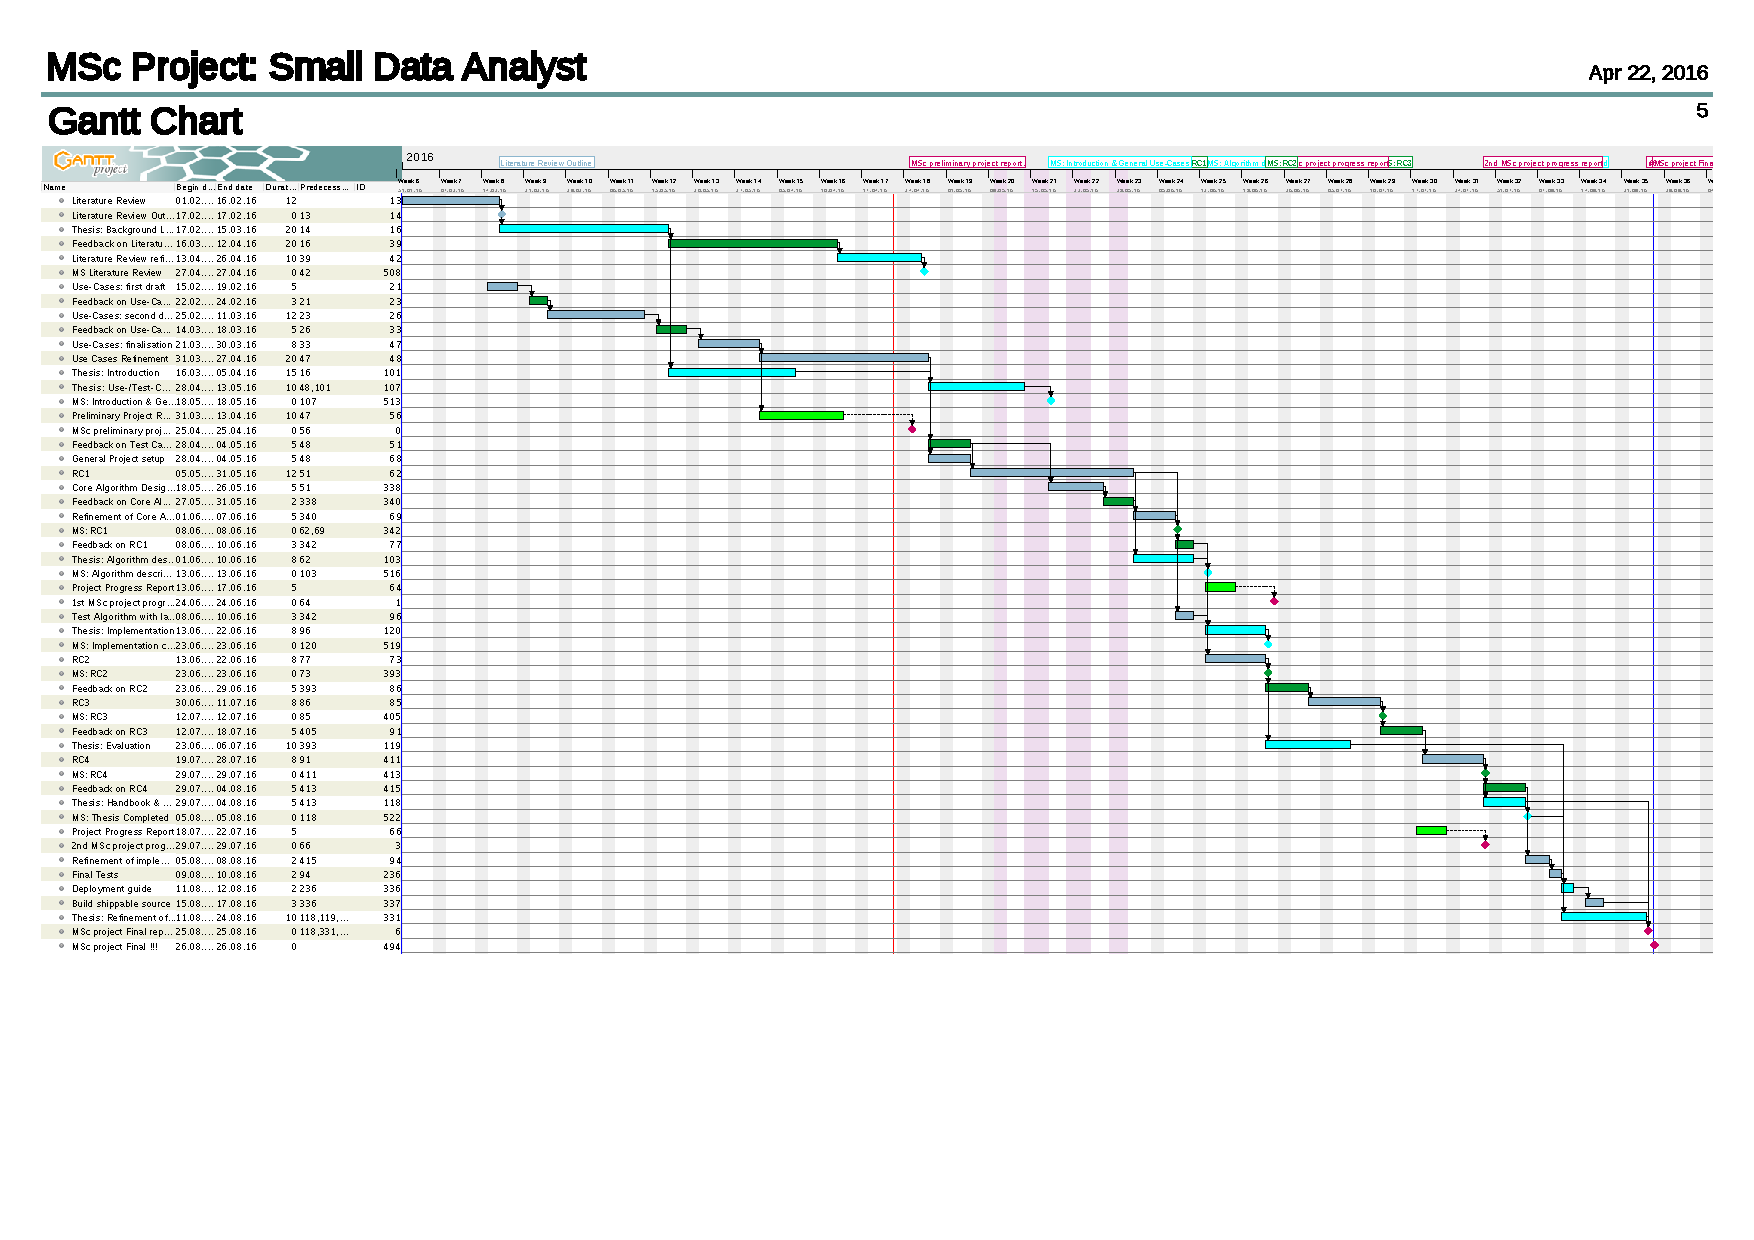
\includegraphics[page=1,width=\textwidth]{appendix/Projectplan.pdf}
	\caption{Project plan for the whole development and research}
	\label{fig:projectplan}
\end{sidewaysfigure}

\section{Software Design Process}
\label{sec:design}

The software design process has been inspired by the Use Case 2.0 \cite{jacobson2011usecase} of Iva Jacobsen \textit{et al.}. This approach is an extension of the \gls{UML} definition for \glspl{use_case} and includes a more specific approach how to deal with different layers of abstraction. This helps to guide the requirement analysis in an efficient way and enables easy communication between software engineers and non-coders. A brief overview of the used approach can be found in \autoref{fig:usecase20:flow}.

\begin{figure}[!ht]
\centering
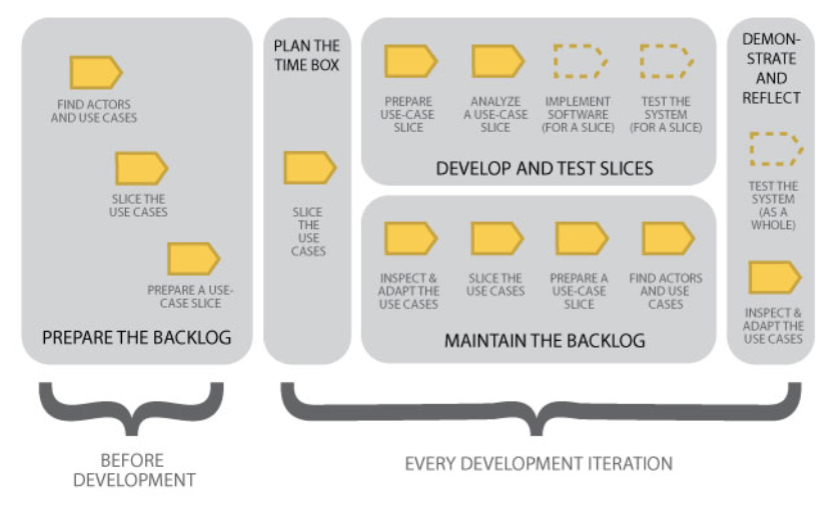
\includegraphics[width=0.8\textwidth]{figures/uc20_flow}
\caption{\gls{use_case} 2.0 activities for iterative development approaches \cite{jacobson2011usecase}}
\label{fig:usecase20:flow}
\end{figure}


\subsection{Use-Cases, Use-Case Flows and Use-Case Slices}
Use cases are the core concept in Use Case 2.0. In addition to the \gls{UML} specification \glspl{use_case} are described as cards including the attributes Priority, Release, Size and Complexity. For the prioritisation the MoSCoW\todo{reference} (Must, Should, Could, Would) is used. After the initial requirement analysis, \glspl{use_case_slice} are generated usually including flows, tests and an estimation of the development. In this step the different \glspl{Actor} are identified and test cases are defined. To do so, the \glspl{use_case_slice} are analysed to check how the system elements will interact to perform the assigned \gls{use_case}. The \glspl{use_case_slice} are then going to be implemented and tested with the previous defined test scenarios. Finally the whole system will be tested with \glspl{e2e_test}.

\textbf{\glspl{use_case}} are the general tasks the system and the actors will perform. They are big, not thought completely through and do not contain directly implementable tasks.

\textbf{\glspl{use_case_flow}} are the different flows, how the interaction between actors and the system take place. Usually there is a standard flow, and alternative (error / exception handling) flows. These will be specified later when we go deeper into the analysis. In the state of Use Case Flows we will as well generate Test Cases for the flows. 

\textbf{\glspl{use_case_slice}} are the final development tasks. They will be generated out of the Use Case Flows and can be independently implemented as a single iteration step. They are bases on the Flows and Test Cases. Further Test Cases are usually generated during the implementation react on system specific scenarios.


\subsection{Test Driven development}
\label{sec:tdd}
\todo{TDD approach}

\subsection{Test Suit}
\label{sub:test_suit}
\todo{Describe test suit}


\section{Specification}
\label{sec:specification}

In accordance with the selected methodology of Use Case 2.0 (see \autoref{sec:design}) no in-depth specification has been written, however a reasonable amount of \glspl{use_case} have been defined and iterativly refined. These were then reviewed by the client and discussed in detail. As mentioned, the project used Trello as management tool. All \glspl{use_case} have been described on cards and \glspl{use_case_slice} have been generated out of those. They are directly reflected by the description in \cite{sassoon2014,sassoon2016, sassoon2016CD}. In general each \gls{use_case} consists of the following attributes: Name, Desired outcome, (Main-)\glspl{Actor}, Flow to achieve the desired outcome, Alternative flow (optional).


\subsection{Weak requirements}
\label{sub:weak}
In addition to the described \glspl{use_case} (see \autoref{tab:usecases}) the following weak requirements influenced the development of the final project:


\begin{itemize}
	\item The system should be designed as an interactive \textbf{web application} to ensure:
	\begin{itemize}
		\item Access for multiple users.
		\item Portability between different operating systems.
		\item No requirement of installation of software on local computers.
		\item Clinician and Statistician can share the same infrastructure without the need of working at the same place.
	\end{itemize}
	\item A decent test suite should be provided to ensure the functionality of the system.
	\item The system must be suitable for different user types (\glspl{Actor}).
	\item The system has to provide different levels of access for different user groups.
	\item The system should be able to execute test scripts as \texttt{R}-Scripts.
	\item The system should be hosted on a free accessible hosting provider.
\end{itemize}


\subsection{Use Cases}
\label{sub:use_cases}
\autoref{tab:usecases} shows an overview over the major \glspl{use_case} that have been generated during the requirements analysis. For the sake of simplicity they have not been integrated into this dissertation. However they are public available on the \href{https://trello.com/b/ywCkicpc}{Trello-Board}\footnote{\url{https://trello.com/b/ywCkicpc}}.

\begin{landscape}
	\begin{longtable}{ l l p{10.5cm} l l p{3cm} }
		\textbf{ID}                         & \textbf{\Gls{Actor}}\footnote{C: Clinician, S: Statistician, A: Admin} &\textbf{Description} &  \textbf{RC} & \textbf{Prio}\footnote{MoSCoW priorities} &  \textbf{Comments}\\
		\href{https://trello.com/c/KEOokZp9}{UC1}   & 	- & 	Enter two default models into the system as code without user interface including definition of assumptions & RC1 & Must &  For initial testing purposes  \\
		\href{https://trello.com/c/ebVrFdA5}{UC2}   & 	C & 	Get models that are appropriate for a research question & RC1	& Must &	   \\
		\href{https://trello.com/c/ORRBjISQ}{UC2-1} & 	C & 	Store done analysis & RC2 & Should &  see \autoref{as:1} \\
		\href{https://trello.com/c/qKLAoWRj}{UC3} 	&  	S & 	Define assumptions for models & - & - & obsolet \\
		\href{https://trello.com/c/7NINsfz8}{UC4}   & 	C & 	Check that a dataset meets the set of assumptions of a model and that the queries to the clinician regarding the research question's  assumptions are met as well. & RC1 & Must   &   \\
		\href{https://trello.com/c/22JGne3r}{UC5}   & 	C & 	Select a research question & RC1 & Must &   \\
		\href{https://trello.com/c/CVGBVWID}{UC6}   &   C, S, A & 	Login into the system and be authenticated with your role & RC2 & Should &	 \\
		\href{https://trello.com/c/pId27kJM}{UC6-1} &   A & 	Create new users & RC2 & Must &	 \\
		\href{https://trello.com/c/pQ98qgSL}{UC6-2} &  	A & 	Delete users & RC2 & Must	 &   \\
		\href{https://trello.com/c/mvxBeNSR}{UC6-3} &  	A & 	Modify users & RC2 & Should &   \\
		\href{https://trello.com/c/DidVQKAS}{UC7}   &   C & 	Fill patient data into the system to be checked by the models & RC2 & Must &  \\
		\href{https://trello.com/c/be2088JH}{UC8}	& 	C & 	See arguments for and agains models for a research question & RC2 & Must &   \\
		\href{https://trello.com/c/Ca9mA3uA}{UC9}   &   C & 	Define new personal preferences & RC3 & Must &   \\
		\href{https://trello.com/c/Ca9mA3uA}{UC9-1}   &   S & 	Define new global preferences & RC3 & Must &   \\
		\href{https://trello.com/c/1s656fA9}{UC10}  &   C & 	Get recommended model taking into account global preferences & RC3 & Should & 	 \\
		\href{https://trello.com/c/xUDStSOK}{UC11}  &   A & 	Create new users with a specific role for the system & RC3 & Could &    \\
		\href{https://trello.com/c/5UMo7o6U}{UC12}  &   S & 	Enter additional analysis models into the system in a defined language as text so that it will be regarded as an option for applicable models	& RC3 & Should & \\
		\href{https://trello.com/c/2V6Cl65u}{UC12-1}&   S & 	Add Test-Argument into the system & RC2 & Must & \\
		\href{https://trello.com/c/OwM2Z7wt}{UC12-2}&   S & 	Add Query-Argument into the system & RC2 & Must &  \\
		\href{https://trello.com/c/VThxB5aS}{UC12-3}&   S & 	Add Test-Query-Assumptions into the system & RC4 & Should & added later\\
		\href{https://trello.com/c/CkpJUNPW}{UC12-4}&   S & 	Run Test-Argument on a specific existing dataset & RC3	& Should &  \\
		\href{https://trello.com/c/Rg6GPnNE}{UC12-5}&   S & 	Add Blank Arguments for grouping of assumptions & RC2 & Could & \\
		\href{https://trello.com/c/ORlMByiQ}{UC13}  &   S & 	Get in-depth information about algorithmic performance & RC4 & Would & rejected\\
		\href{https://trello.com/c/NcV3lo4w}{UC14}  &   C & 	Enter personal preferences for statistical models and/or analysis techniques & RC4 & Could &   \\
		\href{https://trello.com/c/BOUu2hKN}{UC15}  &   C & 	See argumentation frameworks that are generated for/agains the statistical models. Graph Export: See arguments for and agains models for a research question in a nice and graphical &RC4 & Would & 	 ignored as printing of generated graphs possible  \\
		\href{https://trello.com/c/3FCcFdmm}{UC16}  &   C & 	See analysis process of argumentation framework as visualisation & RC4 & Would	&    \\
		\href{https://trello.com/c/Hv2xe2UW}{UC17}  &   S & 	Enter additional research questions into the system & RC3 &Could& \\
		\href{https://trello.com/c/w1YiIgU7}{UC17-1}&   S & 	Modify research questions&RC3 & Must &  \\
		\href{https://trello.com/c/UbT5mtDx}{UC17-2}&   S & 	Delete research questions&RC3&Must& \\
		\href{https://trello.com/c/dpLHOxbB}{UC18}  &   S & 	Include R-script execution	 & RC1 & Must & \\
		\href{https://trello.com/c/bZHdWpkt}{UC19}  &   S & 	Enter global preferences for statistical models and/or analysis techniques& RC3 & Could &	 \\

		\caption{List of the different use cases that have been evaluated during the requirements analysis.}	
		\label{tab:usecases}
	\end{longtable}
\end{landscape}

The \glspl{use_case} defined in \autoref{tab:usecases} were then further defined, requirements deriving from it have been generated as \glspl{use_case_slice} and were implemented by applying an iterative approach with close feedback loops to the supervisor of the project and the author of \cite{sassoon2014,sassoon2016, sassoon2016CD} who has been treated as a \gls{product owner} or client. As the software was developed in a test driven approach (see \autoref{sec:tdd}) all features where implemented by designing tests first. This is reflected by the final existing test suite (see \autoref{sub:test_suit}) which contains a decent amount of \glspl{unit_test}, \glspl{integration_test} and \glspl{e2e_test} and has an overall line coverage of $ \geq 85\%$ (see \href{https://codeclimate.com/github/sebastianzillessen/small-data-analyst/coverage}{https://codeclimate.com/github/sebastianzillessen/small-data-analyst/coverage}). \autoref{uc:12-1} shows an exemplary detailed description of one \gls{use_case}.



{ \tiny
	\begin{longtable}{|p{2cm} p{11cm}|}

		\hline
			\textbf{ID} & 
				\href{https://trello.com/c/2V6Cl65u}{UC12-1}\\
			
			\hline
			\textbf{Actor} & Statistician or Admin \\
			\hline
			\textbf{Description} & 
				Add Test-Argument into the system\\
			\hline
			\textbf{Desired~outcome} & 
				- A statistician can create new arguments \newline
				- These arguments can be assigned to models \newline
				- The arguments are accessible for all users in the system \newline
		\\
		\hline
			\textbf{Flow} & 
				1.) The user is logged in as Admin/Statistician  \newline
				2.) The User clicks on "Add Test-Argument" (see \href{https://trello.com/c/OwM2Z7wt}{Query arguments}, \href{https://trello.com/c/Rg6GPnNE/39-uc12-5-add-attacks-between-arguments}{Blank arguments})\newline
				3.) The system shows a form including "Name", "Description", "Attacking (Model or Other Argument)", "Required data set fields", "R-Code to run test" and a disabled submit button\newline
				4.) The User enters a Name\newline
				5.) The user might enter a description\newline
				6.) The User selects at least on Model or other Argument from the list of possible attacked objects and whether it is critical or non-critical to that object.\newline
				7.) The user enters a list of required data set fields.\newline
				8.) The user enters the R-Code to test if this argument holds or not. The R-Code must return a true/false statement at the end, \texttt{True} saying the argument holds, otherwise \texttt{False}. The R-Script will get as input a variable named \texttt{tabular\_data}  and must assign the variable \texttt{result} with \texttt{true} / \texttt{false} (see \autoref{sec:r_code}). The attributes specified in "Required data set fields" will be checked before executing the \texttt{R}-Script.\newline
				9.) The user is in charge of verifying his script against data sets. A functionality to do so will be given by selecting a data set in the system first. The script will then be checked against this data set.\newline
				10.) The user clicks submit. The system performs a validation of the argument.\newline
				11.) The System stores the argument in the database and redirects the user to a list of available arguments and shows a success message.
		\\
		\hline
			\textbf{Alternatives} & 
							1.a) Not logged in as Admin: No changes to arguments possible.
				\newline	4.a) No name entered: show required inline message, disable submit button.
				\newline	6.a) No attacked object selected: show required inline message, disable submit button.
				\newline	8.a) If the user does not enter a R-Script: mark as required and do not enable submit button.
				\newline	9.a) If there is a syntax error: Show syntax error and line to the user
				\newline	9.b) If the result is not boolean: Show error explaining true/false result required.
				\newline	9.c) If there has been an error during execution with the test data set: show error.
				\newline	9.d) After successful run: Show the data set used to test it and the result.
				\newline	10.a) If the user does not select "Submit": NO changes done.
				\newline	11.a) If the validation fails: Redirect the user back to the form page and show validation failure.
				\newline	11.b) If any error occurs,  Redirect the user back to the form page and show error explanation.
							\\
		\hline

	\label{uc:12-1}\\
	\caption{Use case 12-1: "Add Test-Argument into the system." An example for a detailed description of a use case.}
\end{longtable}
}


\subsection{Actors in our System}
\label{sub:sassoon:actors}
During the requirements analysis the following actors have been identified and are described as follows:

\textbf{Clinicians} are the main users of the system and do the actual analysis of a dataset by using the predefined research questions, models and assumptions. A clinician should see all globally available research questions, models and their assumptions. In addition the preferences defined by the statistician will apply to all analyses a clinician performs. However she/he will be able to enter personal preferences between models that only apply for his analyses. An overview over her/his uses cases can be seen in \autoref{fig:usecase:clinician}.

\textbf{Statisticians} are able to enter statistical models into the system and to define global applicable preferences. To do so, a statistician can enter different types of assumptions mapped to models and preferences. These might contain query assumptions, where the clinician performing an analysis has to confirm a fact, or test assumptions that are checked against the dataset by running a \texttt{R}-script. She or he is as well allowed to see all datasets that have been uploaded and to check which analysis have been performed (see \autoref{fig:usecase:statistician}).



\textbf{Administrators} are able to create, modify and destroy all available data in the system. In addition an administrator is required to approve new users and to assign them to a role. She or he is as well capable of inviting new users into the system. An overview over her/his uses cases can be seen in \autoref{fig:usecase:admin}.



\subsection{Technical Specification}
\label{sub:technical}

As the system should be accessible by multiple users and from different departments (e.g. clinicians and statisticians), it will be developed as a web-application in \gls{RoR}\footnote{\href{http://rubyonrails.org}{http://rubyonrails.org}} and will be hosted on Heroku\footnote{\href{https://www.heroku.com}{www.heroku.com}} as this will provide an easy-to-use and easy-to-deploy environment, where our demo application can be hosted for free. To provide a \gls{CI} environment, the project code is hosted on \texttt{github}\footnote{\href{https://github.com/sebastianzillessen/small-data-analyst}{https://github.com/sebastianzillessen/small-data-analyst}} and a \texttt{Travis CI}\footnote{\href{https://travis-ci.org/sebastianzillessen/small-data-analyst}{https://travis-ci.org/sebastianzillessen/small-data-analyst} } instance has been setup that runs all the implemented tests of the project.

The used datasets are anonymised, so data protection issues are reduced to a minimum and the datasets can be hosted in the cloud. \texttt{PostgreSQL}\footnote{\href{http://www.postgresql.org}{http://www.postgresql.org}} will be used as a database, as it is well integrated on Heroku and provides high scalability.

Most of the assumption tests for the statistical models will be performed in \gls{R}, as this is a common used language for statistical calculations and well known by statisticians. In addition many assumption-checks already exist in \gls{R}. These scripts (externally provided) will be executed in the \gls{RoR} application with the help of third party gems.

To provide a responsive and clear user interface the \texttt{Bootstrap}\footnote{\href{http://getbootstrap.com}{http://getbootstrap.com}} framework will be used to design and style the application. 

\subsection{Data flow in the System}

\autoref{fig:data_flow} shows -- in a simplified representation -- the data flows in the process of statistical model selection: First of all, the statistician has to create global preferences, research questions including their possible models and the required assumptions. This is all stored in a knowledge base which is itself stored in  a persistent database. A detailed description of all database classes can be found in \autoref{sub:db}. 

\begin{figure}[!h]
\centering
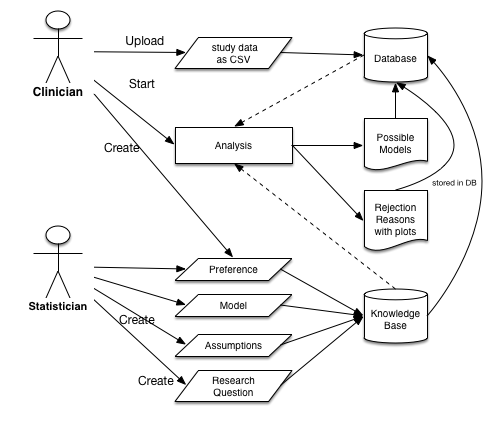
\includegraphics[width=0.8\textwidth]{figures/data_flow}
\caption{Core data flow in the system to create new analyses.}
\label{fig:data_flow}
\end{figure}


A clinician can upload new clinical data retrieved from studies by using the CSV upload functionality. Starting a new analysis retrieves the dataset from the database and instantiates the knowledge base for this specific problem. The assumptions of all applicable models for the selected research question are then evaluated. If multiple models are possible, the preferences (first the globally defined ones by a statistician, later the personal preferences a clinician might have) are applied to the system one after another until one last model remains. This model is then returned as recommended model. The process of the rejection of various models will be graphically visible to the user (see \autoref{sub:ui}). The process of creating and processing a new analysis is described in detail in \autoref{sub:walk}.



\section{Application Overview}
In the following chapter a short introduction to the actual system will be given. An entity relationship diagram explains the core data foundation of this project in \autoref{sub:db}, which includes the representation of the \gls{SKB} as described in \autoref{sub:SKB}. The general process, core functionalities and the gls{ui} will be presented in \autoref{sub:process}-\ref{sub:ui}. This is followed by a typical walkthrough to create a new analysis as a clinician. 

The application is available on \href{https://small-data-analyst.herokuapp.com}{https://small-data-analyst.herokuapp.com} and these steps can be reproduced in the demo application. At the end of this chapter a short discussion on observations is included, providing as well the insight feedback of an actual statistician using the software. A detailed view on some key components of the software can be found in \autoref{sec:implementation}.


To test the application the standard \textit{ovarian}-dataset available in \texttt{R} has been used. In addition to that, I. Sassoon provided an anonymised version of a larger clinical data set (see \autoref{app:dataset}). The description of the dataset can be found in \autoref{fig:dataset}. Possible research question arising from this dataset are presented in \autoref{fig:dataset:rq}.



\subsection{Entity Relationship Class Diagram }
\label{sub:db}


The underlying database structure of the developed application is mostly influenced by the \gls{SKB} and the representation of \texttt{Assumptions} as classes. \autoref{fig:er} shows an overview over most of the involved database models used in this application. Additional classes like \texttt{Users}, \texttt{Abilities}, etc. are intentionally left out as this would add an additional level of complexity. 

\begin{figure}[!h]
	\centering
	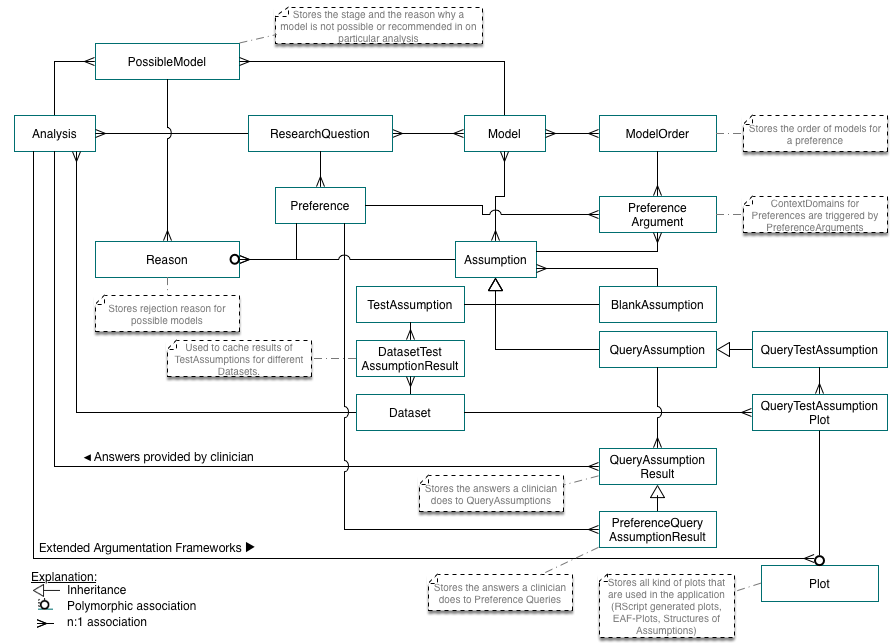
\includegraphics[width=\textwidth]{figures/er_complete}
	\caption{Entity-Relationship Diagram of the major classes used int the application. }
	\label{fig:er}
\end{figure}


The most important class is the \texttt{Analysis} which is associated with a \texttt{Dataset}, a \texttt{ResearchQuestion}, has many answered or open \texttt{QueryAssumptionResults} (this class stores the answers of a clinician to one particular \texttt{QueryAssumption}), and a list of \texttt{PossibleModels} (including impossible models and there \texttt{Reason} why they got rejected). 

The \gls{SKB} is represented by \texttt{ResearchQuestions} that have and belong to many \texttt{Models}. Each of these has multiple \texttt{Assumptions} that need to hold for this \texttt{Model}. These \texttt{Assumptions} have different specialisations: 

\bigskip

\begin{itemize}

	\item \texttt{TestAssumption}: An assumption that requires a \texttt{R} script to be executed and to return \texttt{true} or \texttt{false}. These assumptions will be checked automatically from the system and rely only on the dataset used in an analysis.
	\item \texttt{QueryAssumption}: A clinician has to provide a \textit{yes} or \textit{no} answer to a question during the process of the analysis. Only if he answers positively, this assumption holds.
	\item \texttt{QueryTestAssumption}: A \texttt{R} script generates a plot based on the dataset, which is then presented to the user who has to confirm that the plot shows some required features.
	\item \texttt{BlankAssumption}: An assumption that represents a grouping ability for other assumptions. It holds only if all of it assigned assumptions (regardless of their type) hold. 
\end{itemize}
\bigskip


\texttt{Preferences} have different \texttt{PreferenceArguments} that represent a specific \gls{CD} which are assigned to a particular \texttt{ModelOrder}. This allows the representation of \glspl{CD}, their order and the expressed preferences as described in \autoref{sub:SKB} in a generic way without limiting the triggers for a \gls{CD} to any particular \texttt{Assumption} type. 

The class \texttt{DatasetTestAssumptionResult} stores for each \texttt{TestAssumption} and each \texttt{Dataset} a pre-calculated result to enhance the speed of the evaluation during new \texttt{Analses}. \texttt{PreferenceQueryAssumptionResults} and \texttt{QueryAssumptionResults} store the answers of clinicians to \texttt{(Test)QueryAssumptions} for one particular \texttt{Analysis}.


\subsection{General Process and Application Setup}
\label{sub:process}
The crucial role in the process of enabling clinicians to analyse there clinical data is played by the statistician: registered or approved by an administrator he is allowed to perform significant changes to the \gls{SKB} which is required to provide the clinician with a sophisticated foundation for his analyses. 

\begin{figure}[h]
\centering
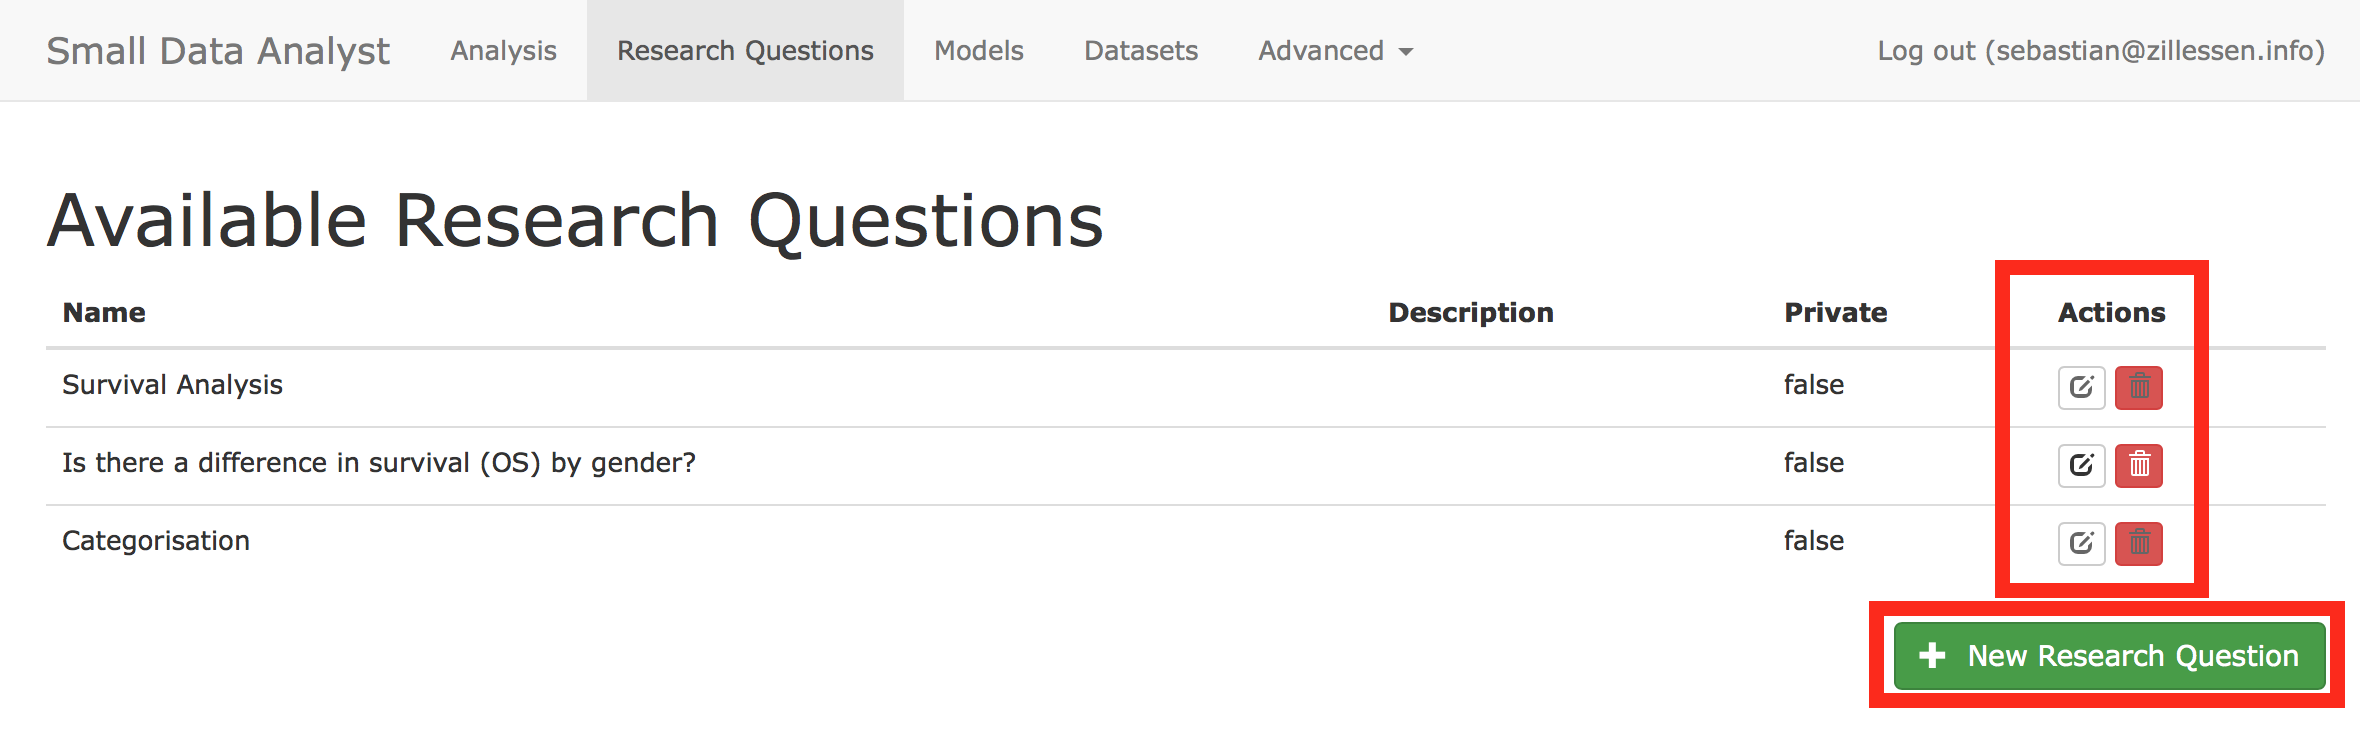
\includegraphics[width=0.8\textwidth]{figures/ui_RQ}
\caption{Listing of research questions: The highlighted areas might not be available, depending on the access rights of the currently logged-in user.}
\label{fig:ui:rq}
\end{figure}

To do so a \textbf{statistician} will first prepare the system involving the following steps:

\begin{enumerate}
	\item Defining a research question (see \autoref{fig:ui:rq}).
	\item Assigning suitable models (see \autoref{fig:ui:model}) to a research question and providing assumptions (see \autoref{fig:ui:assumption}) that need to hold to make this model a possible model in a particular analysis.
	\item Defining (global) preferences to express a particular order between models in certain contexts that apply if a certain assumption holds (see \autoref{fig:ui:preference}).
\end{enumerate}

\bigskip

A \textbf{clinician} can then initialise a new analysis by performing the following steps:
 
\begin{enumerate}
	\item Uploading a dataset that has been acquired during a clinical study.
	\item Optionally expressing (private) preferences between different models.
	\item Generating a new analysis related to a research question and providing the answers required by the system to generate a list of possible models.
	\item Answering further data related questions that might arise during the evaluation of the possible models to apply context domain specific preferences on the dataset.
\end{enumerate}
\bigskip

By applying this workflow, \textbf{clinicians} will be able to make data-driven decisions that are based on the expertise entered by a \textbf{statistician}.


\subsection{User Interface and Core Functionalities}
\label{sub:ui}

The \gls{UI} is intentionally kept clean for simplicity reasons: \texttt{Bootstrap} is used to provide a consistent look \& feel and responsiveness of the application. As described in \autoref{sub:sassoon:actors} we have three main users in our system which have different abilities\footnote{Abilities are access rights, that are specified via an \texttt{Ability} class that is used by \texttt{cancancan} to provide diversified access-rights to different user groups in our system.} influencing the appearance of the \gls{UI} (eg. a clinician will not be able to create, alter or delete any research questions, however he will still be able to see them as depicted in \autoref{fig:ui:rq}). This approach allows us to use the same \gls{UI}-components for different users without writing them once again (\gls{DRY} principle).

\begin{figure}[h]
\centering
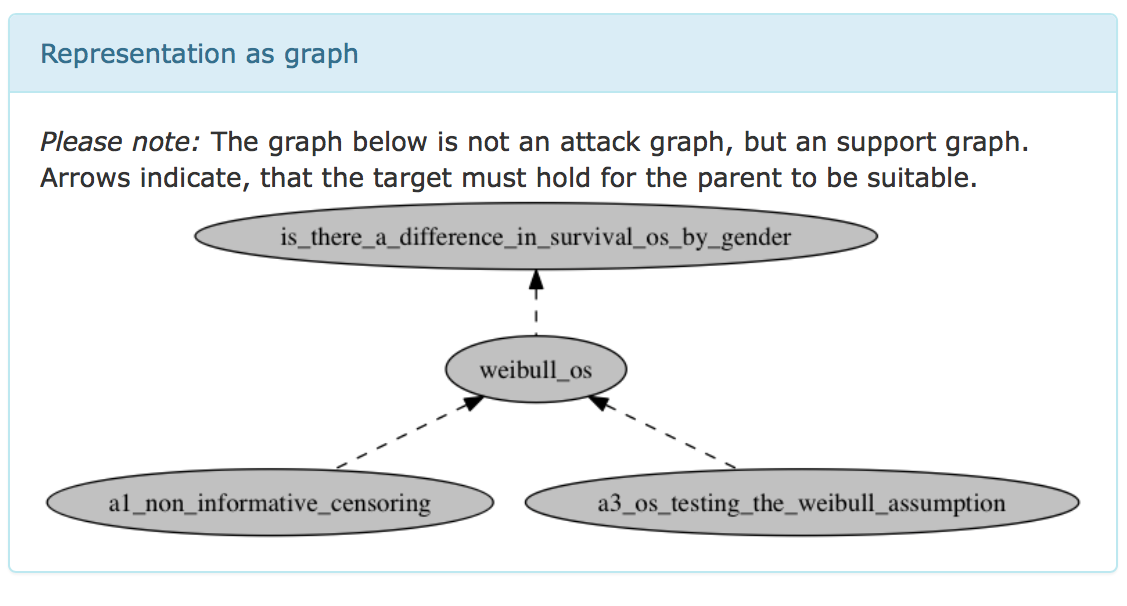
\includegraphics[width=0.8\textwidth]{figures/ui_Weibull_Model}
\caption{Overview over a model, in this particular case the \textit{Weibull model} which requires two assumptions to hold.}
\label{fig:ui:model}
\end{figure}


To provide easier access to the underlying \gls{SKB}, research questions and models include a visual representation of their relations as a graph (see lower right part of \autoref{fig:ui:model}). The system offers four different types of assumptions which have special functionalities (see \autoref{fig:ui:assumption}, explanation of each type can be found in \autoref{sub:db}).

\begin{figure}[t!]
\centering
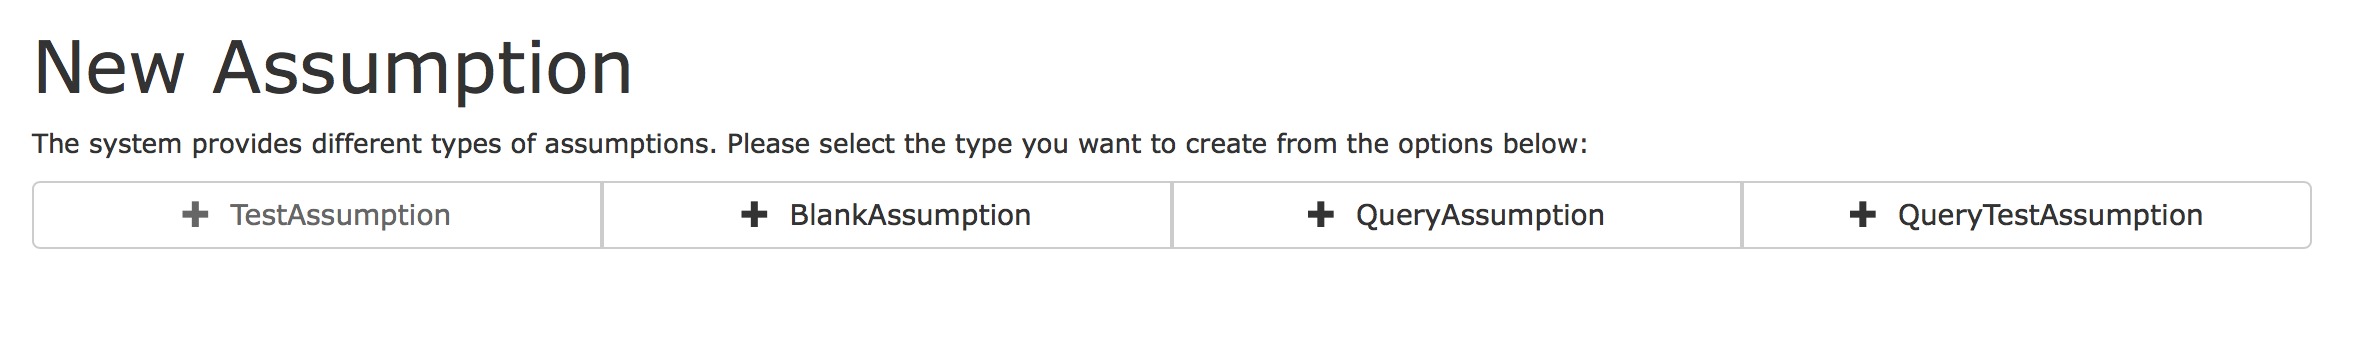
\includegraphics[width=0.8\textwidth]{figures/ui_new_assumption}
\caption{The system provides four different types of assumptions: Test, Query, Test-Query, and Blank assumptions.}
\label{fig:ui:assumption}
\end{figure}

Each of those require different attributes which results in different forms during the creation process of new assumptions. For a model to be possible during an analysis, all assumptions assigned to this model need to hold (evaluate to true) regardless of its type. In a second step, the defined \glspl{preference} are evaluated. To do so, all possible models are added to an \gls{EAF} attacking each other as described in \autoref{sub:preferences} and the \glspl{CD} are then added iteratively. This process can be seen in \autoref{fig:analysis:eaf}.

\begin{figure}[!hbt]
	\centering
	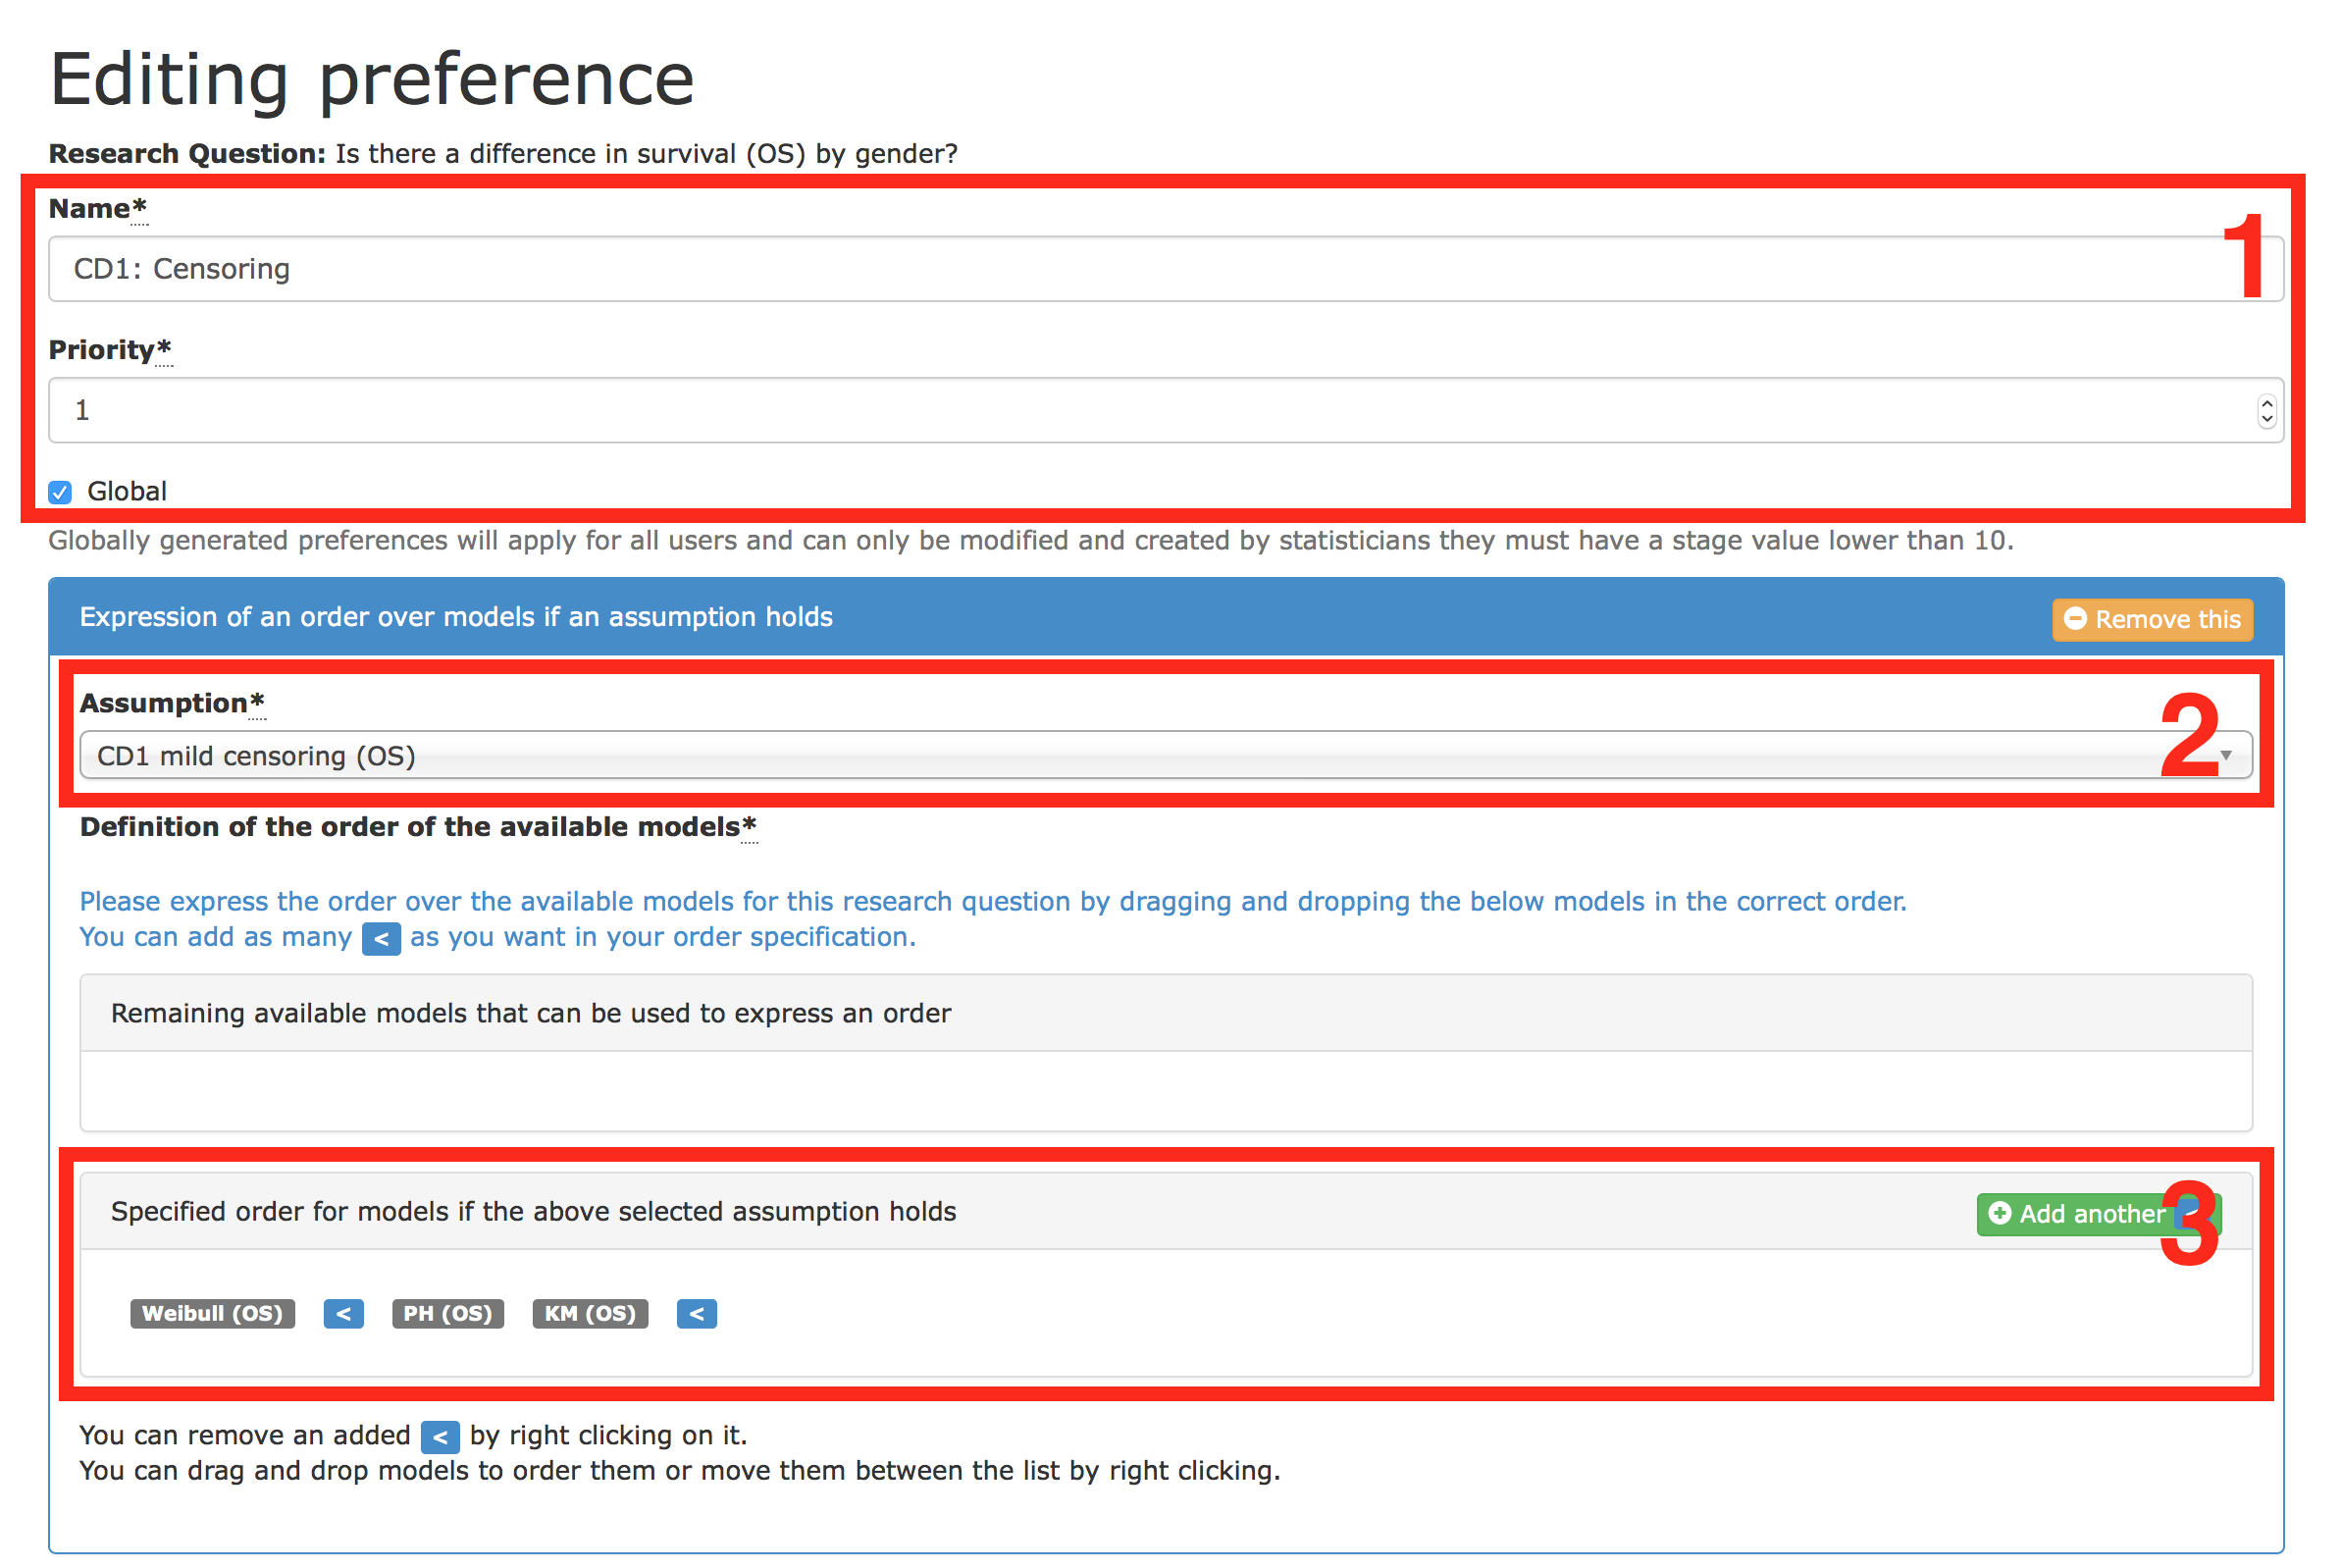
\includegraphics[width=\textwidth]{figures/ui_preference}
	\caption{\gls{UI} to enter preferences between models: General information about this preference including the applicable research question (1), the context under which this preference applies can be defined as assumption (2), and the actual order of the models can be interactively arranged per drag \& drop (3).}
	\label{fig:ui:preference}
\end{figure}


The most complex component from a \gls{UI} perspective are preferences, as they involve context domains and there required assumptions and relative orders per context domain. \autoref{fig:ui:preference} shows how this has been solved: (1) allows the user to enter general details for a preference (availability to users, rank of the preference and a name). 

For each available context domain for this particular preference, an assumption (2) has to be chosen. A context domain will be applied, if and only if this assumption holds. The relatively order between models can be specified easily via drag \& drop (3). This order will be taken into account when analysing the \gls{EAF} at the final step of the analysis process. If a preference is not defined over all available models for a particular research question, the model will not be attacked by any \gls{CD}, therefore the performance measurement for this model is undefined and it will stay untouched.


This overall approach allows \textbf{clinicians} and \textbf{statisticians} to enter their personal preferences into the system, which are managed by a sophisticated rights-management. 

As expressed earlier before, the priority of a preference can be set and defines the order of applying different \glspl{CD}. This ensures, that a clinicians preference will always be less important than the statistical reasons a statistician has entered into the system. This ensures reliability and statistical correctness while applying the preferences on possible models.


\subsection{Example walkthrough}
\label{sub:walk}

In the following a walkthrough for a new analysis involving a sample dataset provided by I. Sassoon (see \autoref{app:dataset}) and a survival analysis by gender (preferences set according to \cite{sassoon2016CD}) is described in detail. These initial options are selected in \autoref{fig:analysis:1}. The following screen (see \autoref{fig:analysis:2}) depicts the actual analysis screen. All \texttt{TestAssumptions} have already been evaluated and on the left hand side of the screenshot the \textit{Currently Possible Models} are depicted. On the right hand side the \textit{Open Query Assumptions} are presented to the user including one \texttt{QueryTestAssumption} with a generated plot for this particular dataset and one \texttt{QueryAssumption}. 

\begin{figure}[b]
	\centering
	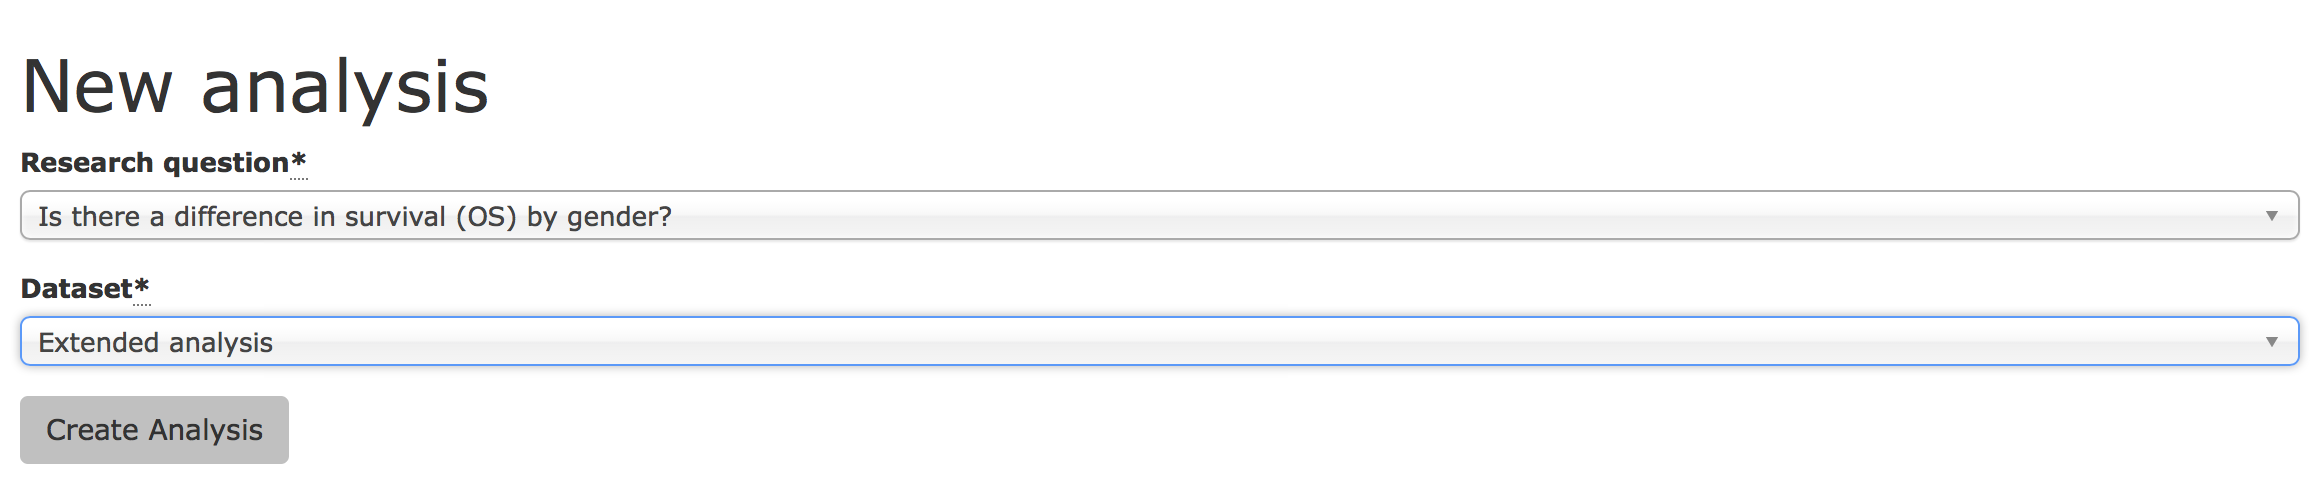
\includegraphics[width=\textwidth]{figures/ui_analysis_0}
	\caption{Creating a new analysis, step 1: Selection of dataset and research question. }
	\label{fig:analysis:1}
\end{figure}

In this particular case, all entered models for the given research question are possible. If one \texttt{TestAssumption} for one of those models would not hold and this model would have further \texttt{Query(Test)Assumptions}, these will not be presented to the end-user, as this model is already not possible anymore. If multiple models require the same answers to one \texttt{QueryAssumption} (e.g. for our example all three models depend on assumption \texttt{A1}) the clinician will only be asked to answer this question once. 

\begin{figure}[t]
	\centering
	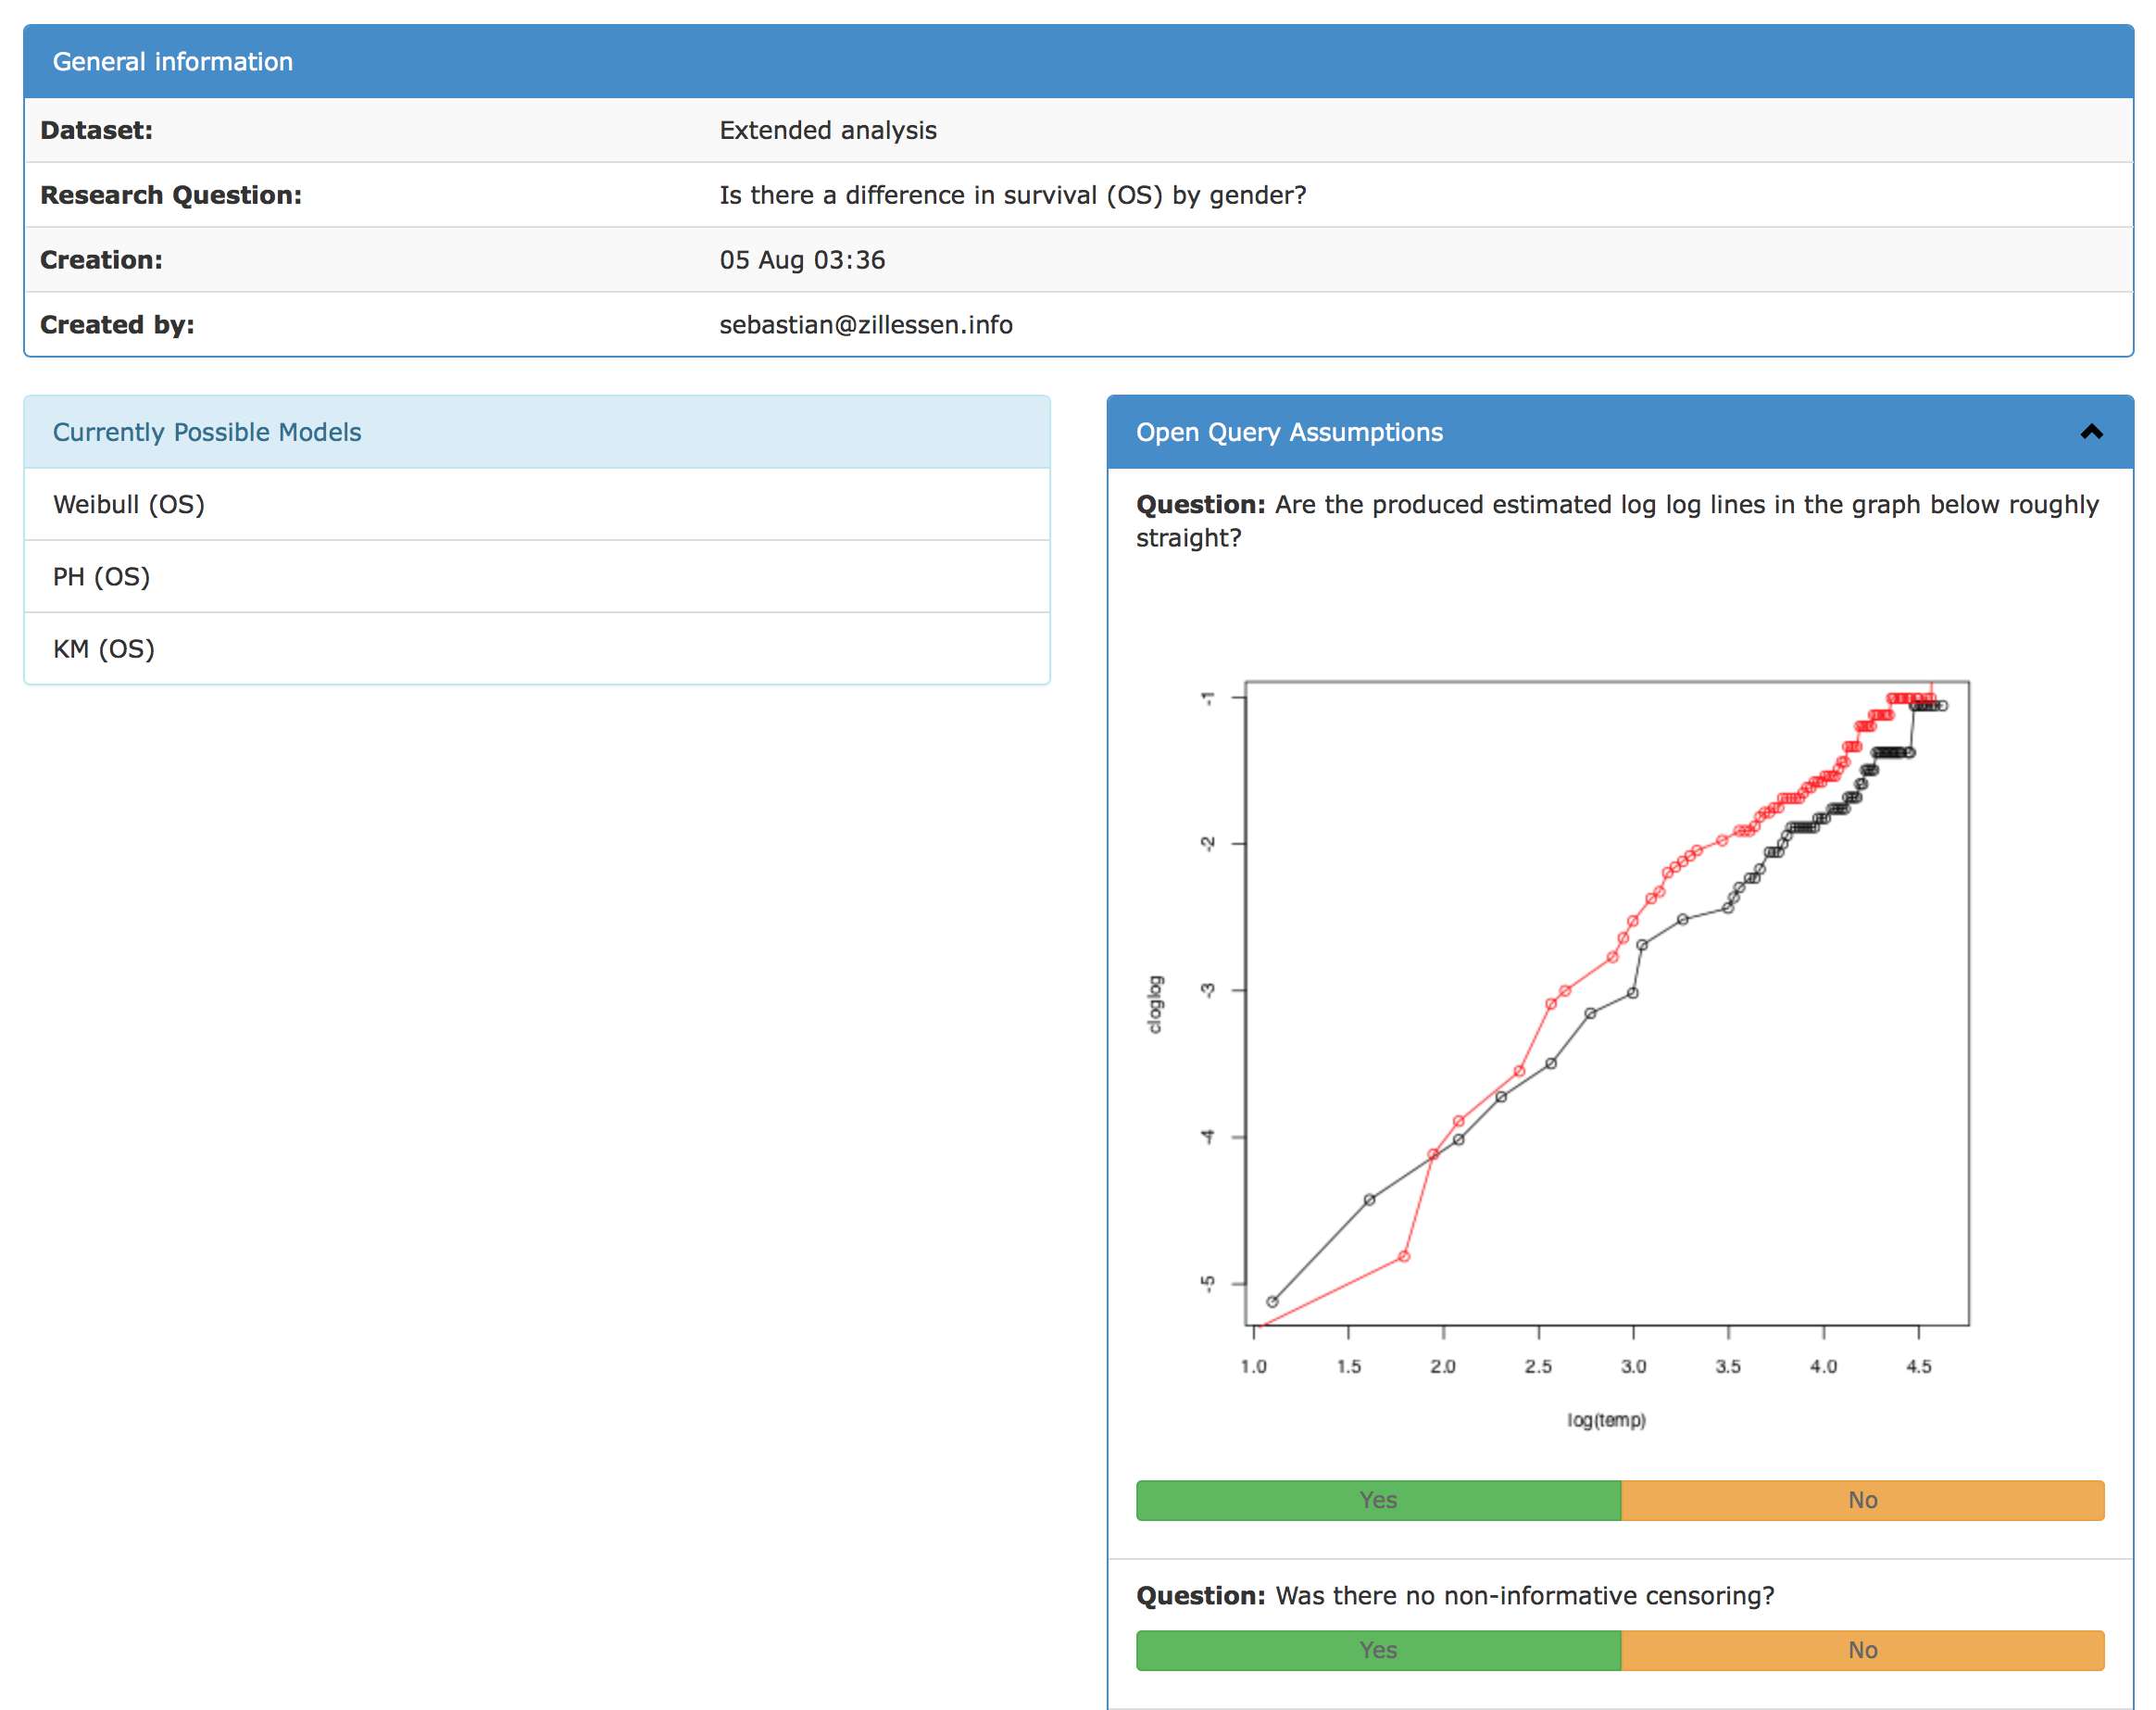
\includegraphics[width=\textwidth]{figures/ui_analysis_1}
	\caption{Creating a new analysis, step 2: Clinician has to answer \texttt{QueryTest-} and \texttt{QueryAssumptions} to perform the analysis. \texttt{TestAssumptions} have already been evaluated.}
	\label{fig:analysis:2}
\end{figure}


As soon as the clinician answers one of the \texttt{QueryAssumptions} the analysis will be updated according to this answer and if some of the \texttt{QueryAssumptions} that are already visible to the user get obsolet by this answer, they will be removed from the open- and moved to the ignored-list (right lower part of \autoref{fig:analysis:3_no}). 
As the clinician answered \texttt{A1} with \textit{No}, the analysis results in no possible models, so no preferences are employed and the analysis is finished.

\begin{figure}[t]
	\centering
	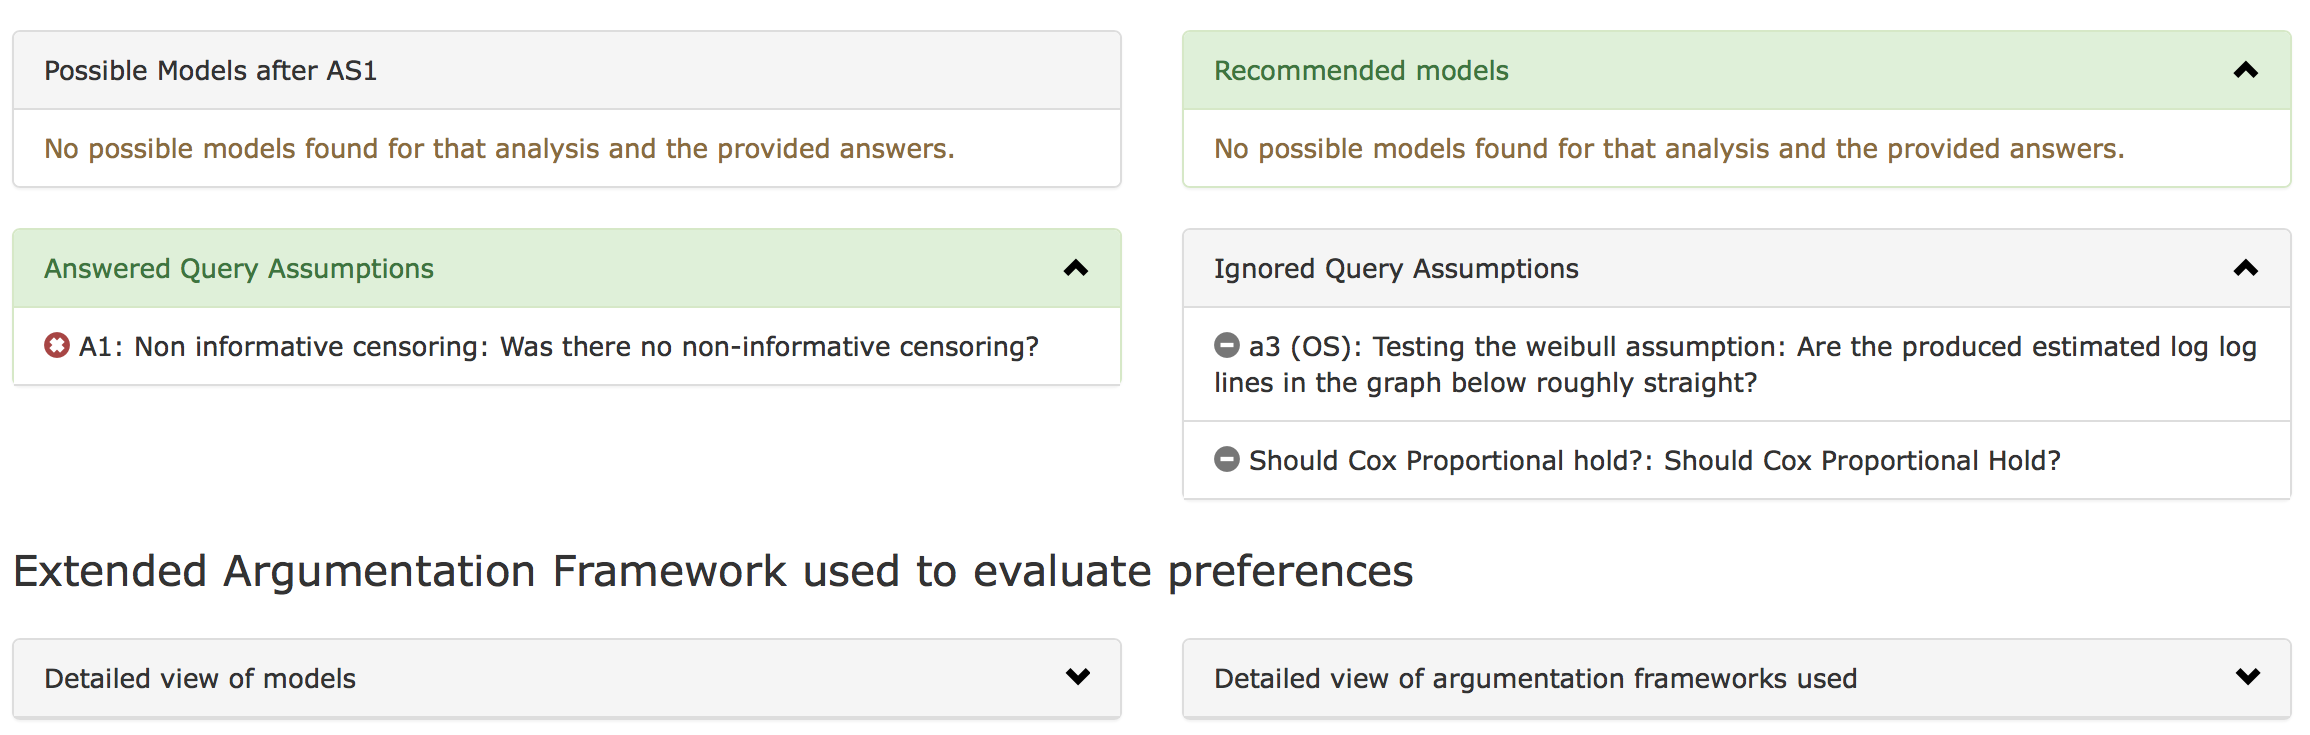
\includegraphics[width=\textwidth]{figures/ui_analysis_2_no}
	\caption{Creating a new analysis, step 3: After answering one question (e.g. "Has no non-informative censoring been in place?" with \textit{No}), the possible models are updated and outdated \texttt{QueryAssumptions} might be removed from the list of queries.}
	\label{fig:analysis:3_no}
\end{figure}

However, if all \texttt{QueryAssumptions} have been answered positively all three models remain possible. The system will now initiate the \gls{EAF} for this particular analysis as described in \autoref{sub:statistical_model_selection}. The evaluation of this \gls{EAF} is performed in the same order: First, the \texttt{TestAssumptions} are evaluated. Second, if no final solution of the \gls{EAF} could be found the \texttt{Query(Test)Assumptions} required for the first preference evaluated accordingly to the \gls{CD} are presented to the user. This process is then repeated with the remaining preferences and their \glspl{CD}.

\begin{figure}[t]
	\centering
	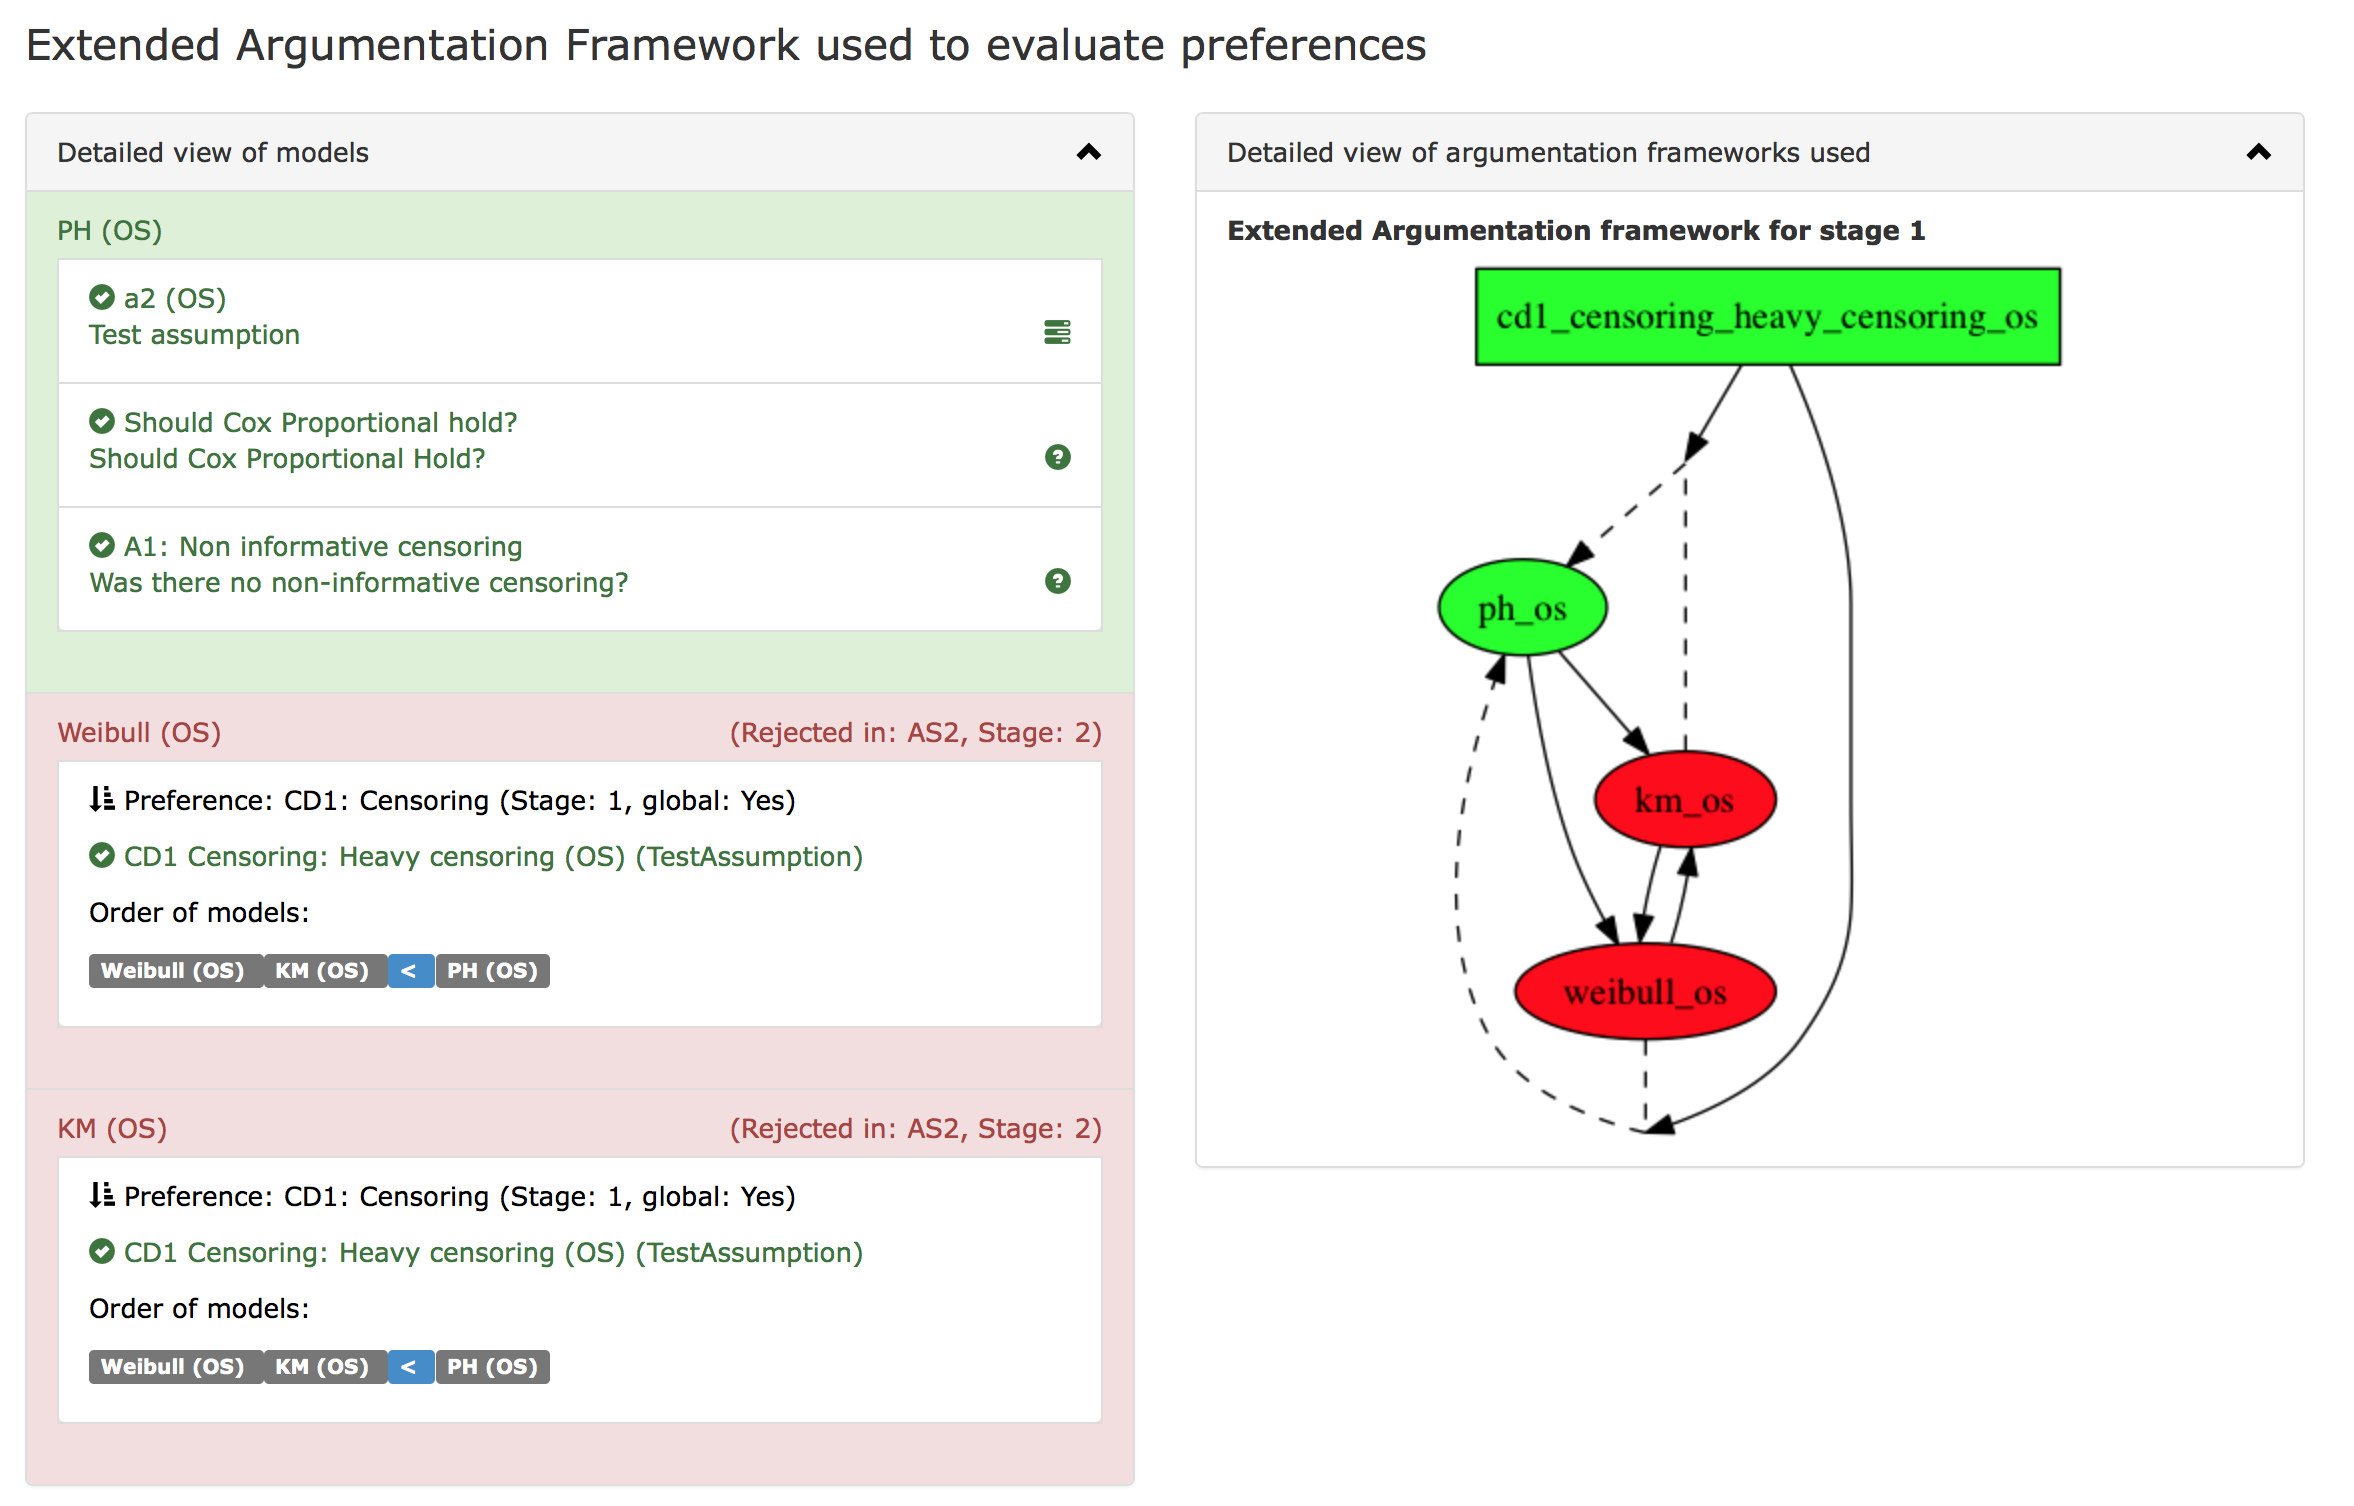
\includegraphics[width=\textwidth]{figures/ui_analysis_eaf}
	\caption{Finished analysis with applied preferences on it: context domain "Censoring" evaluated to \textit{heavy censoring}. }
	\label{fig:analysis:eaf}
\end{figure}


During the evaluation of the preferences per \gls{CD} \textit{Kaplan-Meier} and \textit{Weibull} models are wiped-out as "\textit{Censoring}" has the performance measurement \textbf{heavy}. The generated \gls{EAF} on the right side of \autoref{fig:analysis:eaf} shows the reason why only \textit{Cox-Proportional hazard} remains as the last preferred model.


During the whole process the \gls{UI} provides an interactive way of communication and as it updates its content instantly the user gets direct feedback on his interaction. In addition, the user is not required to answer all questions in a row, the analysis will still be stored in the system and can be continued at any later time. 





\subsection{Observation and Discussion}

The final application provides an intuitive and easy-to-use approach to perform statistical model selection based on properties of the underlying data, statistical theory, and global and personal preferences. This allows statisticians with a deeper knowledge of statistical theory to provide there expertise to clinicians with the in-depth knowledge about the acquisition and external properties of a dataset. 

As global preferences, models including their assumptions and research questions only have to be entered once into the system and as this is done by a statistician the workload for clinicians is reduced to a minimum. This allows them to focus on the actual analysis of the underlying data and equips them with a low-barrier tool, that they might be more likely to use over a longer period of time which leads ultimately to a continuous data-driven decision process

From a statistical perspective, this approach is way more sophisticated as it allows only well educated statisticians to enter the \gls{SKB}, which is so critical for reliable and well informed selection processes. \todo{reference on isabels paper}

\todo{feedback of an actual statistician}



\todo{Main Result:  The chapter reports the contribution of your work.  For example, it could contain the following sub-sections to summarise the contribution of the project: Theoretical Development, Analysis and Design, Implementation and Experimental Work, Results, Observation and Discussion.}

\section{Implementation Details}
\label{sec:implementation}
In the following section, some implementation details will be highlighted. An entity relationship diagram explains the core data foundation of this project in \autoref{sub:db}, which represents the \gls{SKB} as described in \autoref{sub:SKB}. Overall the development of the intelligent agent could be accomplished with general techniques and features (such as the \gls{MVC} architecture) provided by \gls{RoR}. However, the details of the components related to \glspl{EAF} (see \autoref{sub:eaf_algorithm}) and \glspl{AF} (see \autoref{sub:af_algorithm}) should be highlighted, as they are crucial for the successful implementation. The requirements for \gls{R}-scripts entered into the application will be presented in \autoref{sec:r_code}.
	

	%\todo{Program listings (depending on the project nature). Complete source code listings must be submitted as an appendix to the report (excluding any well-known, freely obtainable, third-party libraries explicitly mentioned in the report). In addition, the source code must be submitted in a compressed file via KEATS together with the report. You should try to help the reader to navigate through your source code by providing a "table of contents" (titles of these files/units and one line descriptions). The first page of the program listings folder must contain the following statement certifying the work as your own: "I verify that I am the sole author of the programs contained in this folder, except where explicitly stated to the contrary". Your (typed) signature and the date should follow this statement.}

\subsection{Entity Relationship Class Diagram }
\label{sub:db}


The underlying database structure of the developed application is mostly influenced by the \gls{SKB} and the representation of \texttt{Assumptions} as classes. \autoref{fig:er} shows an overview over most of the involved database models used in this application. Additional classes like \texttt{Users}, \texttt{Abilities}, etc. are intentionally left out as this would add an additional level of complexity. 

\begin{figure}[!h]
	\centering
	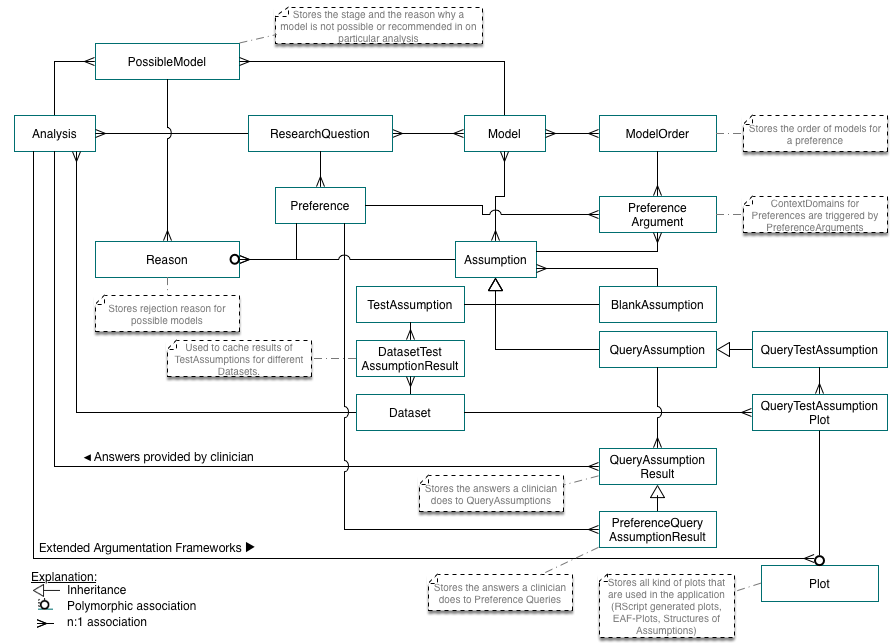
\includegraphics[width=\textwidth]{figures/er_complete}
	\caption{Entity-Relationship Diagram of the major classes used int the application. }
	\label{fig:er}
\end{figure}


The most important class is the \texttt{Analysis} which is associated with a \texttt{Dataset}, a \texttt{ResearchQuestion}, has many answered or open \texttt{QueryAssumptionResults} (this class stores the answers of a clinician to one particular \texttt{QueryAssumption}), and a list of \texttt{PossibleModels} (including impossible models and there \texttt{Reason} why they got rejected). 

The \gls{SKB} is represented by \texttt{ResearchQuestions} that have and belong to many \texttt{Models}. Each of these has multiple \texttt{Assumptions} that need to hold for this \texttt{Model}. These \texttt{Assumptions} have different specialisations: 

\bigskip

\begin{itemize}

	\item \texttt{TestAssumption}: An assumption that requires a \texttt{R} script to be executed and to return \texttt{true} or \texttt{false}. These assumptions will be checked automatically from the system and rely only on the dataset used in an analysis.
	\item \texttt{QueryAssumption}: A clinician has to provide a \textit{yes} or \textit{no} answer to a question during the process of the analysis. Only if he answers positively, this assumption holds.
	\item \texttt{QueryTestAssumption}: A \texttt{R} script generates a plot based on the dataset, which is then presented to the user who has to confirm that the plot shows some required features.
	\item \texttt{BlankAssumption}: An assumption that represents a grouping ability for other assumptions. All assigned assumptions (regardless of their type) must hold. 
\end{itemize}
\bigskip


\texttt{Preferences} have different \texttt{PreferenceArguments} that represent a specific \gls{CD} which are assigned to a particular \texttt{ModelOrder}. This allows the representation of \glspl{CD}, their order and the expressed preferences as described in \autoref{sub:SKB} in a generic way without limiting the triggers for a \gls{CD} to any particular \texttt{Assumption} type. 

The class \texttt{DatasetTestAssumptionResult} stores for each \texttt{TestAssumption} and each \texttt{Dataset} a pre-calculated result to enhance the speed of the evaluation during new \texttt{Analses}. \texttt{PreferenceQueryAssumptionResults} and \texttt{QueryAssumptionResults} store the answers of clinicians to \texttt{(Test)QueryAssumptions} for one particular \texttt{Analysis}.


\subsection{Extended Argumentation Framework: Algorithm}
\label{sub:eaf_algorithm}

An algorithm to solve \glspl{EAF} was presented in \cite{Dunne10computationin} (see \cref{fig:eaf_algo}) and is used to solve acceptability w.r.t. a subset $S' \subseteq \X$ of an argument $x \in \X$ in an \gls{EAF}. The presented algorithm defines an \gls{EAF} as a triple $\langle \X, \A, \D \rangle$ (\autoref{sub:eaf} introduced it as $\langle \S, \R, \D \rangle$).
This algorithm transforms an \gls{EAF} into an \gls{AF} using a colouring-based approach. To do so, it eliminates the attack-on-attacks relation $\D$ by removing elements from $\A$ according to the provided subset $S'$. In addition, \cref{fig:af_algo} (see \cref{sub:af_algorithm}) will be applied to check whether $x$ is acceptable w.r.t. $S'$ in the resulting AF $\langle \X', \A' \rangle$\footnote{As the \gls{EAF} gets reduced to an \gls{AF} the following is true: $\X' \subseteq \X, \A' \subseteq \A$.}.


\begin{algorithm}[htbp]
	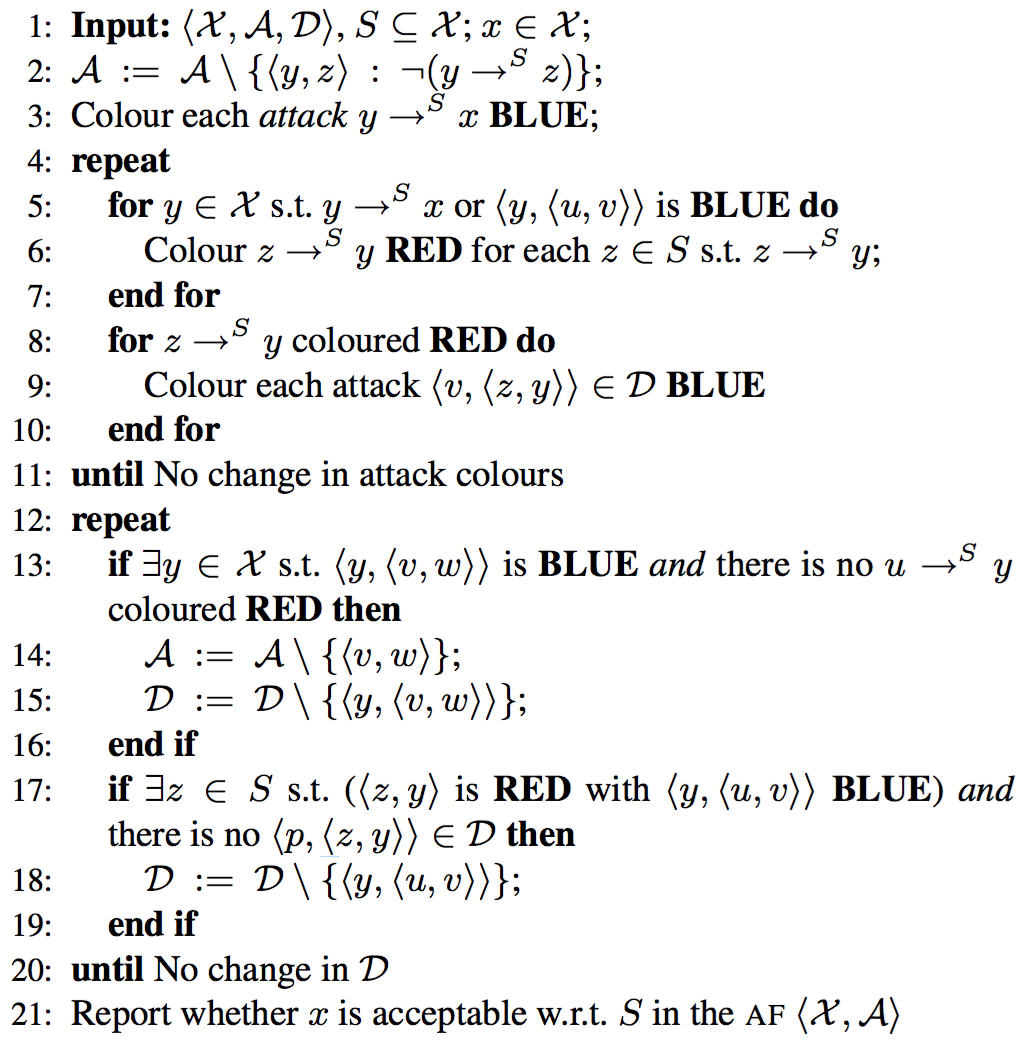
\includegraphics[width=0.7\textwidth]{figures/eaf_algorithm}
	\caption{Deciding \gls{EAF} Acceptability of $x \in \X$ w.r.t. $S' \subseteq \X$ in $\langle \X, \A, \D \rangle$.}
	\label{fig:eaf_algo}
\end{algorithm}


\subsection{Argumentation Framework: Algorithm}
\label{sub:af_algorithm}

The algorithm presented in \cref{fig:af_algo} is based on an labelling approach proposed in \cite{Modgil2009Proof, rodrigues}. It is supposed to calculate the preferred extensions of an \gls{AF}. \texttt{Cand} holds the possible candidates for a preferred labelling as defined in \cref{def:preferred_extension} and is initialised with \texttt{Cand = $\emptyset$}. The Ruby implementation of this algorithm can be found in \cref{lst:af}. The used class \texttt{Labelling} can be found in the provided source code. 

\begin{algorithm}[hbtp]
	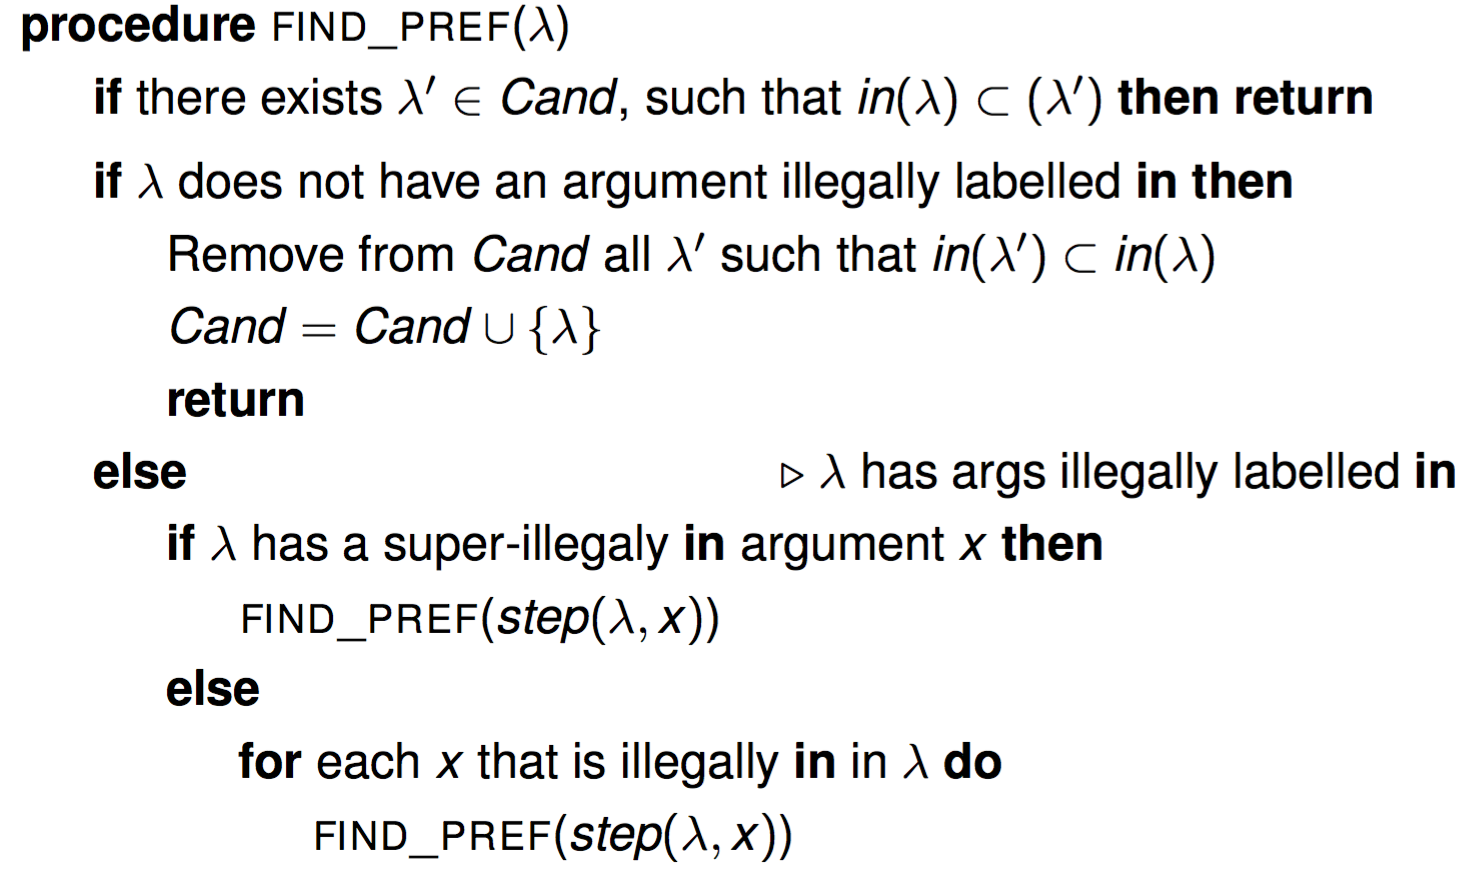
\includegraphics[width=0.7\textwidth]{figures/af_labelling}
	\caption{Algorithm to compute preferred labellings $\lambda \in $ \texttt{Cand} for \glspl{AF} \cite{rodrigues}.}
	\label{fig:af_algo}
\end{algorithm}



\subsection{R-Code and \texttt{rinruby} Gem}
\label{sec:r_code}

To test if a \texttt{TestAssumption} holds or not, statisticians have to upload \gls{R}-scripts that verify these assumptions on the selected data set. This is done by executing the script in \gls{R} and returning the result back to the \gls{RoR} application. Therefore the scripts have to fulfil certain criteria to be able to communicate correctly with the rest of the agent. The provided scripts are executed using regular R-Syntax. In addition to the by default loaded libraries, the \texttt{survival} library will be installed on the executing systems, as it is often used during analyses related to statistical model selection.

Accessing the data set of the analysis as an input in the R-script is essential. The application supports only uploads of CSV files. Thereby the selected format of providing the data sets to the scripts was chosen to be a tabular representation as \gls{R} has an excellent support of loading CSV files.

\begin{listing}[tbp]
	\rcode{figures/mild_censoring.r}
	\caption{R-script to evaluate a \texttt{TestAssumption} on a data set to check whether the underlying data set has been mild censored or not. The performance measurement of CD1 relies on this check (see \autoref{tab:cd1}). }
	\label{lst:cd_mild}
\end{listing}


Each script that is executed will have access to the variable \texttt{tabular\_data}, which has been initialised with \texttt{tabular\_data=read.csv(file='\#\{filename\}')}. This type of assumption must return its result (whether the assumption holds on this data set or not) in the boolean variable named \texttt{result}. The provided example in \cref{lst:cd_mild} shows, how this \texttt{tabular\_data} and the \texttt{result} variable are used together to perform an assumption check on the data set.

A \texttt{QueryTestAssumption} will receive the additional variable \texttt{fileName}, which is initialised with an absolute filename to a temporary file. This must be used to store a generated plot during the analysis, as the hosted application does not have read and write access to all folders. For this type of assumption it is necessary to return a valid PNG at the provided file location. Please note, that due to some rendering issues, the Heroku hosted installation only supports PNG generation in R-scripts when the \texttt{type} is set to \texttt{cairo} (see \cref{lst:rcode}).

To execute the \gls{R}-scripts the gem \texttt{rinruby}\footnote{\url{https://github.com/clbustos/rinruby}} has been used. As the original gem did not provide all required functionalities and features it has been extended and forked at \href{https://github.com/sebastianzillessen/rinruby}{https://github.com/sebastianzillessen/rinruby}. 

In addition to this, separate so called buildpacks have been used to enable \gls{R}\footnote{\url{https://github.com/virtualstaticvoid/heroku-buildpack-r}} and the generation of plots\footnote{\url{https://github.com/weibeld/heroku-buildpack-graphviz.git}} on Heroku. 



%{\color{gray}
\section{Involved Data}
\subsection{Actual Data}
The data makes use of a small data set used to illustrate the use of survival analysis methodologies when teaching the subject. The data set is called ovarian and contains the survival in a randomised trial comparing two treatments for ovarian cancer. This has 26 cases and the following columns:
\begin{itemize}

\item futime: survival\footnote{Survival in days while not observing the event} or censoring time\footnote{Patient left the observation after this amount of time and the event didnt take place}
\item fustat: censoring status \footnote{"1" indicates that the event has been observed at time $futime$, "0" that the event has not been observed until $futime$}
\item age: of the patient in years
\item resid.ds: residual disease present (1=no, 2=yes) 
\item rx: treatment group (integers)
\item ecog.ps: ECOG performance status (see \autoref{tab:ecog})
\end{itemize}

\subsection{Statistical Knowledge Base}
\begin{itemize}
	\item Models are suitable for research questions
	\item models have critical assumptions
	\item Models have non-critical assumptions (might be violated and can still be alright to use
	\item \texttt{m2 must fulfil the following critical assumptions ["a1", "a2"], ... }\insertref{Isabels follow up paper of example and data and models}
	\item Survival can be achieved by using the following model \texttt{\{"m1"=>"a1", "m2"=>["a1", "a2"], "m3" =>["a1", "a3"]\}}
	\item Assumptions met given ($a_i$). Then we use AS1 (see \autoref{as:1})
	\item R-Code (execution in Ruby possible \cite{rinRuby}  \insertref{https://github.com/clbustos/rinruby} \footnote{\texttt{rinruby} is a gem, that enables evaluation of R code in ruby}) and required outcomes for it decide, whether this model $m_i$ is possible or not. 
	\item In Argumentation for Decision Support\cite{Atkinson2006} an approach using values in the AF is presented, where $A2$ defeats $A1$ iff $A2$ attacks $A1$ and $val(A2) \ngtr_a val(A1)$ which is not applicable as no strict partial order given.
\end{itemize}

}

%\include{contents/main}
\section{Conclusion}
\label{sec:conclusion}
The goal of this project was to implement an already existing theoretical approach described in \cite{sassoon2016, sassoon2014, sassoon2016CD} by developing an intelligent agent, which is capable suggesting appropriate models to the end-user (usually a clinician). During the analysis of a particular data set different assumptions of these models must be evaluated to decide which are applicable. Furthermore, the application should present the relevant arguments for and against the various possible models  for a specific research question. To resolve the problem of defeasible and contradictory preferences between these models, different initialisations of multiple \glspl{EAF} based on \glspl{CD} have been used as described in \cite{sassoon2016, sassoon2016CD}.

The developed web-application provides an intuitive and easy-to-use approach to perform statistical model selection based on properties of the underlying data, statistical theory, as well as global and personal preferences. This allows statisticians with a deeper knowledge of statistical theory to provide their expertise to clinicians with insights about the acquisition and external properties of a data set. 

As a statistician has to enter the \gls{SKB} only once the workload for clinicians is reduced to a minimum. This allows them to focus on the actual analysis of the underlying data and equips them with a low-barrier tool, that they might be more likely to use over a longer period of time, which leads ultimately to a continuous data-driven decision process. As clinicians might not always be qualified to select the appropriated statistical models during the design stage of a study \cite{sassoon2014} a support-agent is essential for a data-driven process.

Only well known and acknowledged techniques have been used to evaluate the (extended) argumentation frameworks, which provides a well-founded root for the overall decision process. In addition graphical representations of the used frameworks have been added to the web-application to provide easy access to the argumentation techniques, especially if they are not familiar to the end-user.

As described in \autoref{sub:outlooks}, the application could be improved by adding the functionality to provide data-provenance by providing "dynamic" \gls{R}-scripts (scripts that are binding to a mapping of database columns instead of names). 

As the underlying work of I. Sassoon \cite{sassoon2016CD} is still in progress, it is likely that further strategies regarding the selection of possible models and evaluating their preferences over one and another will be developed. As the application\footnote{Published under the \href{https://opensource.org/licenses/MIT}{MIT license}.} is written in the well-known framework \gls{RoR} and includes a sophisticated test suite, changes and extensions are easily possible.
 
Although the requirements for the project changed slightly (see \autoref{sub:preferences}) the agile software development process and the defined \glspl{use_case} allowed to react flexible on these changes and provided a good source for discussions with the supervisor and the scientific assistant of this project, which lead to no significant delays during the development process.


%TC:ignore

%%%%% References
\bibliographystyle{ieeetr}
%\bibliographystyle{kclharvardv1}
%%%%% Use King's College Harvard V1 style
% If you want to use a bibliography style that is quite close to 
% the King's College Harvard V1 style (http://libguides.kcl.ac.uk/reference/KingsHarvardV1): 
% 1. Remove or comment the line "\bibliography{ieeetr}" above.
% 2. Provide "kclharvardbib" as a document class parameter in the beginning of this file.
% 3. Uncomment the line "\bibliographystyle{kclharvardv1}" below.
%%%%%

\bibliography{bibs/sassoon, bibs/dung, bibs/hunter_a, bibs/Gorogiannis2009, bibs/dexa06, bibs/Ai-Modern, bibs/modgil, bibs/amgoud, bibs/reiter, bibs/bench, bibs/amgoud98,bibs/tandf_tncl207_25} 


%%%%% Declaration
\todo{Include declaration}
%\thispagestyle{empty}


\mbox{}\newline\vspace{10mm} \mbox{}
\LARGE
{\bf Declaration} 
\normalsize 
\vspace{5mm}

I declare that this thesis is the solely effort of the author.
I did not use any other sources and references than the listed ones. I have marked all contained direct or indirect statements from other sources as such.

Neither this work nor significant parts of it were part of another review process.
I did not publish this work partially or completely yet.
The electronic copy is consistent with all submitted copies.

\bigskip
\bigskip
\bigskip
\bigskip


Signature and date: 






%%%%% Appendix
\appendix

\section{Appendix}
\label{app:a}

\subsection{Other Approaches for Preferences in Argumentation Frameworks}
\label{app:other_afs}
\label{sub:paf}
Other approaches to deal with preferences in argumentation frameworks have been proposed by \cite{amgoud,amgoud1998,Bench2003,pollock1987, prakken1997}. A \gls{PAF} defined in \cite{amgoud1998} is  a triple $\langle \S, \R, Pref \rangle$ where $Pref$ is a (partial of complete) order preordering on $\S \times \S$. The difference between this approach and the one we use is mostly the requirement of a strict ordering that has to be associated with $Pref$ and must be explicitly defined.

Modgil \textit{et al.} introduce in \cite{Modgil2009} the concept of a special class of \textit{hiearchical \glspl{EAF}}, which are defined by the existence of a partition of $\Delta$ into multiple regular Dung argumentation frameworks. Due to this restriction it is possible to define a least fix point of the characteristic function $F$, hence defining the grounded extension $GE(\Delta)$ in the same way, as it has been defined in Dung's framework. However, this is a to narrow restriction for our purposes, therefore this will not be described here. 

\label{sub:vaf}

\Glspl{VAF} as proposed in \cite{Bench2003} define an argumentation framework as a 5-tuple: $\langle \S, \R, V, val, P \rangle$ ($\S$: Arguments, $\R$: Attack relation, $V$: nonempty set of values, $val(\cdot): \S \rightarrow V$: value mapping function, $P$: set of audiences $\{a_1, ..., a_n\}$ where each audience names a total ordering $>_{a_i}$ on $V \times V$). By referring to one specific audience we retrieve a \gls{aVAF}. The set of audiences $P$ is introduced to be able to make use of preferences between values in $V$, so we might have as many audiences as there are orderings on $V$. The new definition of an argument that defeats another argument takes into account the audience $a$ and the $val(\cdot)$ of both arguments to define successful attacks. This approach requires a value mapping function $val(\cdot)$ and doesn't argue with preferences in a natural way. 

However, \cite{Modgil2009} proves that an \gls{aVAF} can be transferred to an \textit{equivalent} \gls{EAF} by representing the \gls{aVAF} with three layers: The outer layer expressing the audience, the second layer expressing the pairwise orderings on values in $V$, and the inner layer based on the actual arguments and attacks in the \gls{aVAF}.

Defeasible reasoning and preferences and their impact on argumentation frameworks are formalised as logical formalism by \cite{pollock1987, prakken1997} in the underlying logical formalism which will be used to instantiate a regular Dung framework.

\subsection{Sample Clinical Data Set}
\label{app:dataset}
{
	\centering
	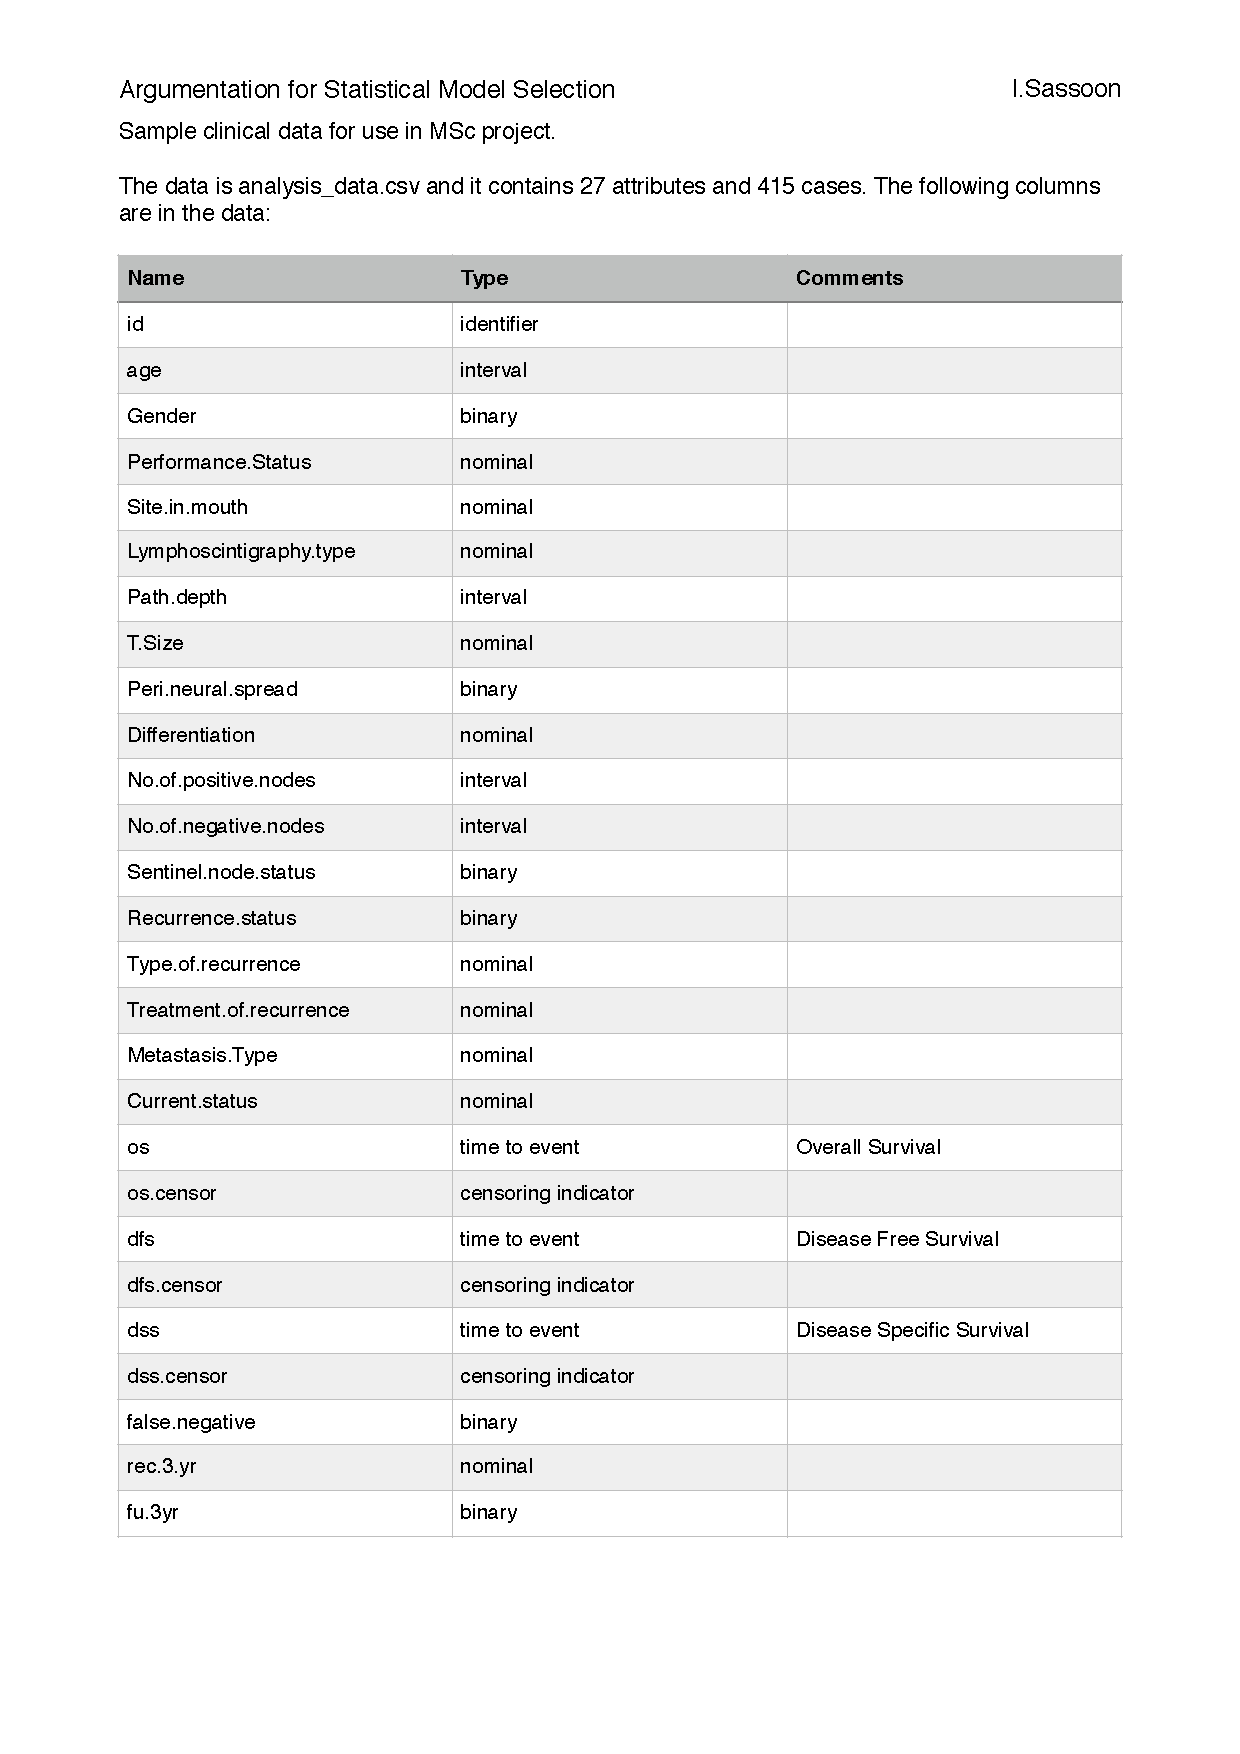
\includegraphics[page=1,width=0.85\textwidth]{appendix/analysis_data.pdf}
	\captionof{figure}{
	Explanation of the example data set provided by I. Sassoon (private email conversation)
	\label{fig:dataset}
	}

	\includegraphics[page=2,width=0.85\textwidth]{appendix/analysis_data.pdf}
	\captionof{figure}{Possible research questions arising from the example data set provided by I. Sassoon (private email conversation)
		\label{fig:dataset:rq}
	}
}



\section{Software related Appendix}
\label{app:b}
\subsection{Code Samples}

\begin{listing}[H]
	\centering
	\rubycode{figures/eaf_to_af.rb}	
	\caption{Ruby Code to implement \autoref{fig:eaf_algo}.}
	\label{lst:eaf}
\end{listing}

\begin{listing}[H]
	\centering
	\rubycode{figures/find_pref.rb}	
	\caption{Ruby Code to implement the labelling based approach $FIND\_PREF$ presented in \autoref{fig:af_algo}.}
	\label{lst:af}
\end{listing}

\begin{listing}[hbtp]
	\rcode{figures/weibull_test.r}
	\caption{R-script to perform a \texttt{QueryTestAssumption} on a data set to check whether the Weibull-Model is applicable or not. The script generates a plot that will be stored in \texttt{fileName} and presented to the end-user.}
	\label{lst:rcode}
\end{listing}


\subsection{Installation Guide}
\label{app:installation}
The following installation guide has been tested on a clean debian OS:

\begin{enumerate}
\def\labelenumi{\arabic{enumi}.}
\item
  Install \texttt{postgresql} and \texttt{R} with:
  \texttt{sudo\ apt-get\ install\ postgresql\ r-base}
\item
  Install \texttt{rvm} following \href{https://rvm.io/rvm/install}{this
  guide}.
\item
  Clone the repository:\\
  \texttt{git\ clone\ }\url{https://github.com/sebastianzillessen/small-data-analyst.git}
\item
  \texttt{cd\ small-data-analyst}
\item
  Install the required ruby version as prompted by rvm:
  \texttt{rvm\ install\ ruby-2.2.4}
\item
  Install bundler: \texttt{gem\ install\ bundler\ foreman}
\item
  Install all required gems: \texttt{bundle\ install}
\item
  Set the AWS credentials in the file \texttt{.env}:

\begin{verbatim}
PORT=3000
AWS_ACCESS_KEY_ID=XXXXXXXXXXXXX
AWS_SECRET_ACCESS_KEY=YYYYYYYYYYYYYYYYYYYY
S3_BUCKET_NAME=ZZZZZZZZZZZZZZ
\end{verbatim}
\item Set the database credentials if required in \texttt{config/database.yml}.
\item
  Initialise the database:\\
  \texttt{rake\ db:create\ \&\&\ rake\ db:setup\ \&\&\ rake\ db:migrate}
\item
  Start the server with \texttt{foreman\ start}
\item
  Create an Admin user:

\begin{verbatim}
$ rails console
> u = User.create(email: "test1@test.de", password: "fooPassword", 
		approved: true, role: :admin)
> u.confirm!
\end{verbatim}
\item
  Navigate to \texttt{http://localhost:3000} and play around with the
  application.
\end{enumerate}


\subsection{Use Cases}
\label{app:use_cases}

Figures \ref{fig:usecase:clinician}, \ref{fig:usecase:statistician} and \ref{fig:usecase:admin} provide an overview over the implemented \glspl{use_case} in the application grouped by their main actors. A complete list of all use cases can be found for further references under \href{https://trello.com/b/ywCkicpc/msc-small-data-analyst}{https://trello.com/b/ywCkicpc/msc-small-data-analyst}.

% use_cases
{
	\centering
	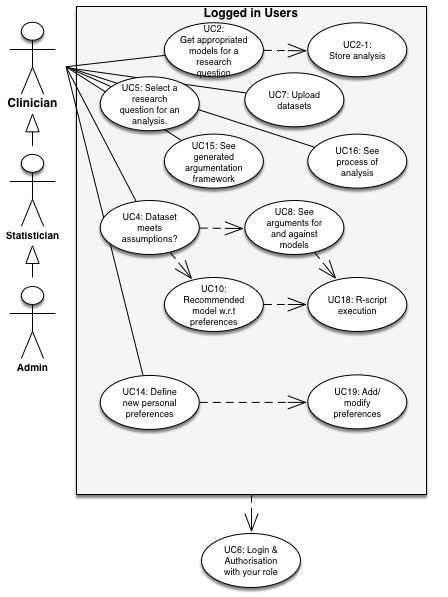
\includegraphics[width=0.6\textwidth]{figures/use_case_clinician}
	\captionof{figure}{Use Case overview for clinicians \label{fig:usecase:clinician}}
	
	
	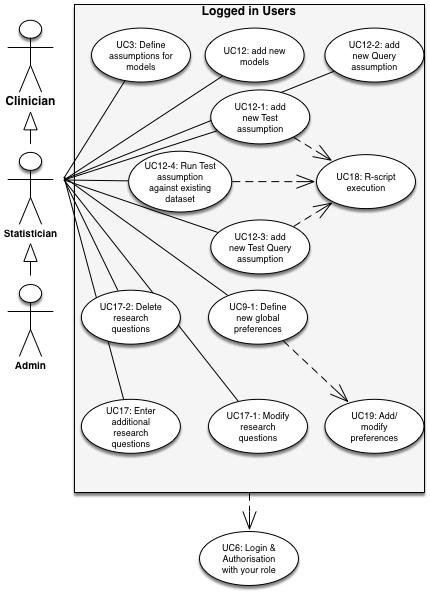
\includegraphics[width=0.6\textwidth]{figures/use_case_statistician}
	\captionof{figure}{Use Case overview for statisticians \label{fig:usecase:statistician}}
	
	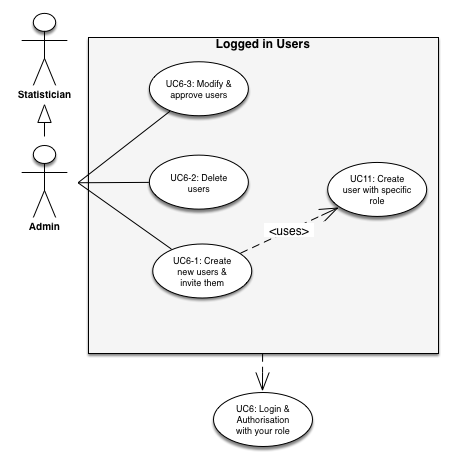
\includegraphics[width=0.6\textwidth]{figures/use_case_admin}
	\captionof{figure}{Use Case overview for administrators \label{fig:usecase:admin}}

}

\section{Third Party Libaries}
\label{app:c}
\label{app:3rdparty}
\autoref{tab:libs} contains all the third party libraries that have been used in the project. These are all public available and free of use. Additional information can be found for each listed \texttt{gem} under \href{http://rubygems.org}{http://rubygems.org}.

\begin{table}[!h]
	\centering
	\begin{tabular}{|p{2.4cm}r||p{2.4cm}r||p{2.4cm}r|}
	\hline
	\textbf{Library} & \textbf{ver.} & 	\textbf{Library} & \textbf{ver.} & 	\textbf{Library} & \textbf{ver.} \\
	actionmailer&(4.2.6)&faker&(1.6.3)&rails\_12factor&(0.0.3)\\
actionpack&(4.2.6)&foreman&(0.82.0)&\tiny{rails\_serve\_static\_assets}&(0.0.5)\\
actionview&(4.2.6)&formtastic&(3.1.4)&\tiny{rails\_stdout\_logging}&(0.0.5)\\
activejob&(4.2.6)&\tiny{formtastic-bootstrap}&(3.1.1)&railties&(4.2.6)\\
activemodel&(4.2.6)&globalid&(0.3.6)&rake&(11.2.2)\\
activerecord&(4.2.6)&haml&(4.0.7)&rdoc&(4.2.2)\\
activesupport&(4.2.6)&haml-rails&(0.9.0)&ref&(2.0.0)\\
addressable&(2.4.0)&heroku-api&(0.4.2)&responders&(2.2.0)\\
arel&(6.0.3)&html2haml&(2.0.0)&\tiny{rootapp-rinruby}&(3.1.2)\footnote{https://github.com/sebastianzillessen/rinruby}\\
aws-sdk&(2.4.2)&i18n&(0.7.0)&rspec-core&(3.4.4)\\
aws-sdk-core&(2.4.2)&jbuilder&(2.5.0)&\tiny{rspec-expectations}&(3.4.0)\\
\tiny{aws-sdk-resources}&(2.4.2)&jmespath&(1.3.1)&rspec-mocks&(3.4.1)\\
bcrypt&(3.1.11)&jquery-rails&(4.1.1)&rspec-rails&(3.4.2)\\
\tiny{binding\_of\_caller}&(0.7.2)&\tiny{jquery-turbolinks}&(2.1.0)&rspec-retry&(0.4.5)\\
builder&(3.2.2)&jquery-ui-rails&(5.0.5)&rspec-support&(3.4.1)\\
bullet&(5.1.1)&json&(1.8.3)&ruby-graphviz&(1.2.2)\\
bundler&(1.12.5)&launchy&(2.4.3)&ruby\_parser&(3.8.2)\\
byebug&(9.0.5)&less&(2.6.0)&rush&(0.6.8)\\
cancancan&(1.15.0)&less-rails&(2.7.1)&sass&(3.4.22)\\
capybara&(2.7.1)&libv8&(3.16.*)&sass-rails&(5.0.4)\\
\tiny{capybara-screenshot}&(1.0.13)&loofah&(2.0.3)&sdoc&(0.4.1)\\
choice&(0.2.0)&mail&(2.6.4)&session&(3.2.0)\\
cliver&(0.3.2)&method\_source&(0.8.2)&sexp\_processor&(4.7.0)\\
cocoon&(1.2.9)&\tiny{mime-types}&(3.1)&\tiny{shoulda-matchers}&(3.1.1)\\
\tiny{codeclimate-test-reporter}&(0.6.0)&\tiny{mime-types-data}&(3.2016*)&simplecov&(0.12.0)\\
coderay&(1.1.1)&mini\_portile2&(2.1.0)&\tiny{simplecov-html}&(0.10.0)\\
coffee-rails&(4.1.1)&minitest&(5.9.0)&slop&(3.6.0)\\
coffee-script&(2.4.1)&multi\_json&(1.12.1)&sprockets&(3.6.2)\\
\tiny{coffee-script-source}&(1.10.0)&nokogiri&(1.6.8)&sprockets-rails&(3.0.4)\\
commonjs&(0.2.7)&orm\_adapter&(0.5.0)&teaspoon&(1.1.5)\\
\tiny{concurrent-ruby}&(1.0.2)&pg&(0.18.4)&\tiny{teaspoon-jasmine}&(2.3.4)\\
data\_migrate&(2.1.0)&pkg-config&(1.1.7)&therubyracer&(0.12.2)\\
\tiny{database\_cleaner}&(1.5.3)&poltergeist&(1.10.0)&thor&(0.19.1)\\
debug\_inspector&(0.0.2)&pry&(0.10.3)&thread\_safe&(0.3.5)\\
delayed\_job&(4.1.2)&puma&(3.4.0)&tilt&(2.0.5)\\
\tiny{delayed\_job\_active\_record}&(4.1.1)&rack&(1.6.4)&turbolinks&(2.5.3)\\
devise&(4.1.1)&\tiny{rack-mini-profiler}&(0.10.1)&\tiny{twitter-bootstrap-rails}&(3.2.2)\\
diff-lcs&(1.2.5)&rack-test&(0.6.3)&tzinfo&(1.2.2)\\plec
docile&(1.1.5)&rails&(4.2.6)&uglifier&(3.0.0)\\
dotenv&(2.1.1)&\tiny{rails-assets-chosen}&(1.6.1)&uniform\_notifier&(1.10.0)\\
dotenv-rails&(2.1.1)&\tiny{rails-assets-jquery}&(3.0.0)&warden&(1.2.6)\\
erubis&(2.7.0)&\tiny{rails-deprecated\_sanitizer}&(1.0.3)&web-console&(2.3.0)\\
excon&(0.51.0)&\tiny{rails-dom-testing}&(1.0.7)&\tiny{websocket-driver}&(0.6.4)\\
execjs&(2.7.0)&rails-erd&(1.4.7)&\tiny{websocket-extensions}&(0.1.2)\\
factory\_girl&(4.7.0)&\tiny{rails-html-sanitizer}&(1.0.3)&workless&(1.2.3)\\
factory\_girl\_rails&(4.7.0)&&&&\\
	\hline
	\end{tabular}
	\caption{Third-party libraries and services used in the web-application.}
	\label{tab:libs}
\end{table}

\clearpage
\newpage

\section{R-Spec Test Suite}
\label{app:d}
\label{app:rspec}
\sloppy
\autoref{sub:test_suit} provides an impression on the developed \texttt{rspec} tests. Only the first two pages have been generated. The whole report can be found on \href{https://github.com/sebastianzillessen/small-data-analyst/blob/master/report.html}{https://github.com/sebastianzillessen/small-data-analyst/blob/master/report.html}. The test suite which is made out of $\approx 350$ specs results in a resonable test coverage of $\geq 85\%$ (see \href{https://codeclimate.com/github/sebastianzillessen/small-data-analyst/coverage}{https://codeclimate.com/github/sebastianzillessen/small-data-analyst/coverage} for in depth code climate details and coverage report).
% rspec
\begin{sidewaysfigure}[!h]
	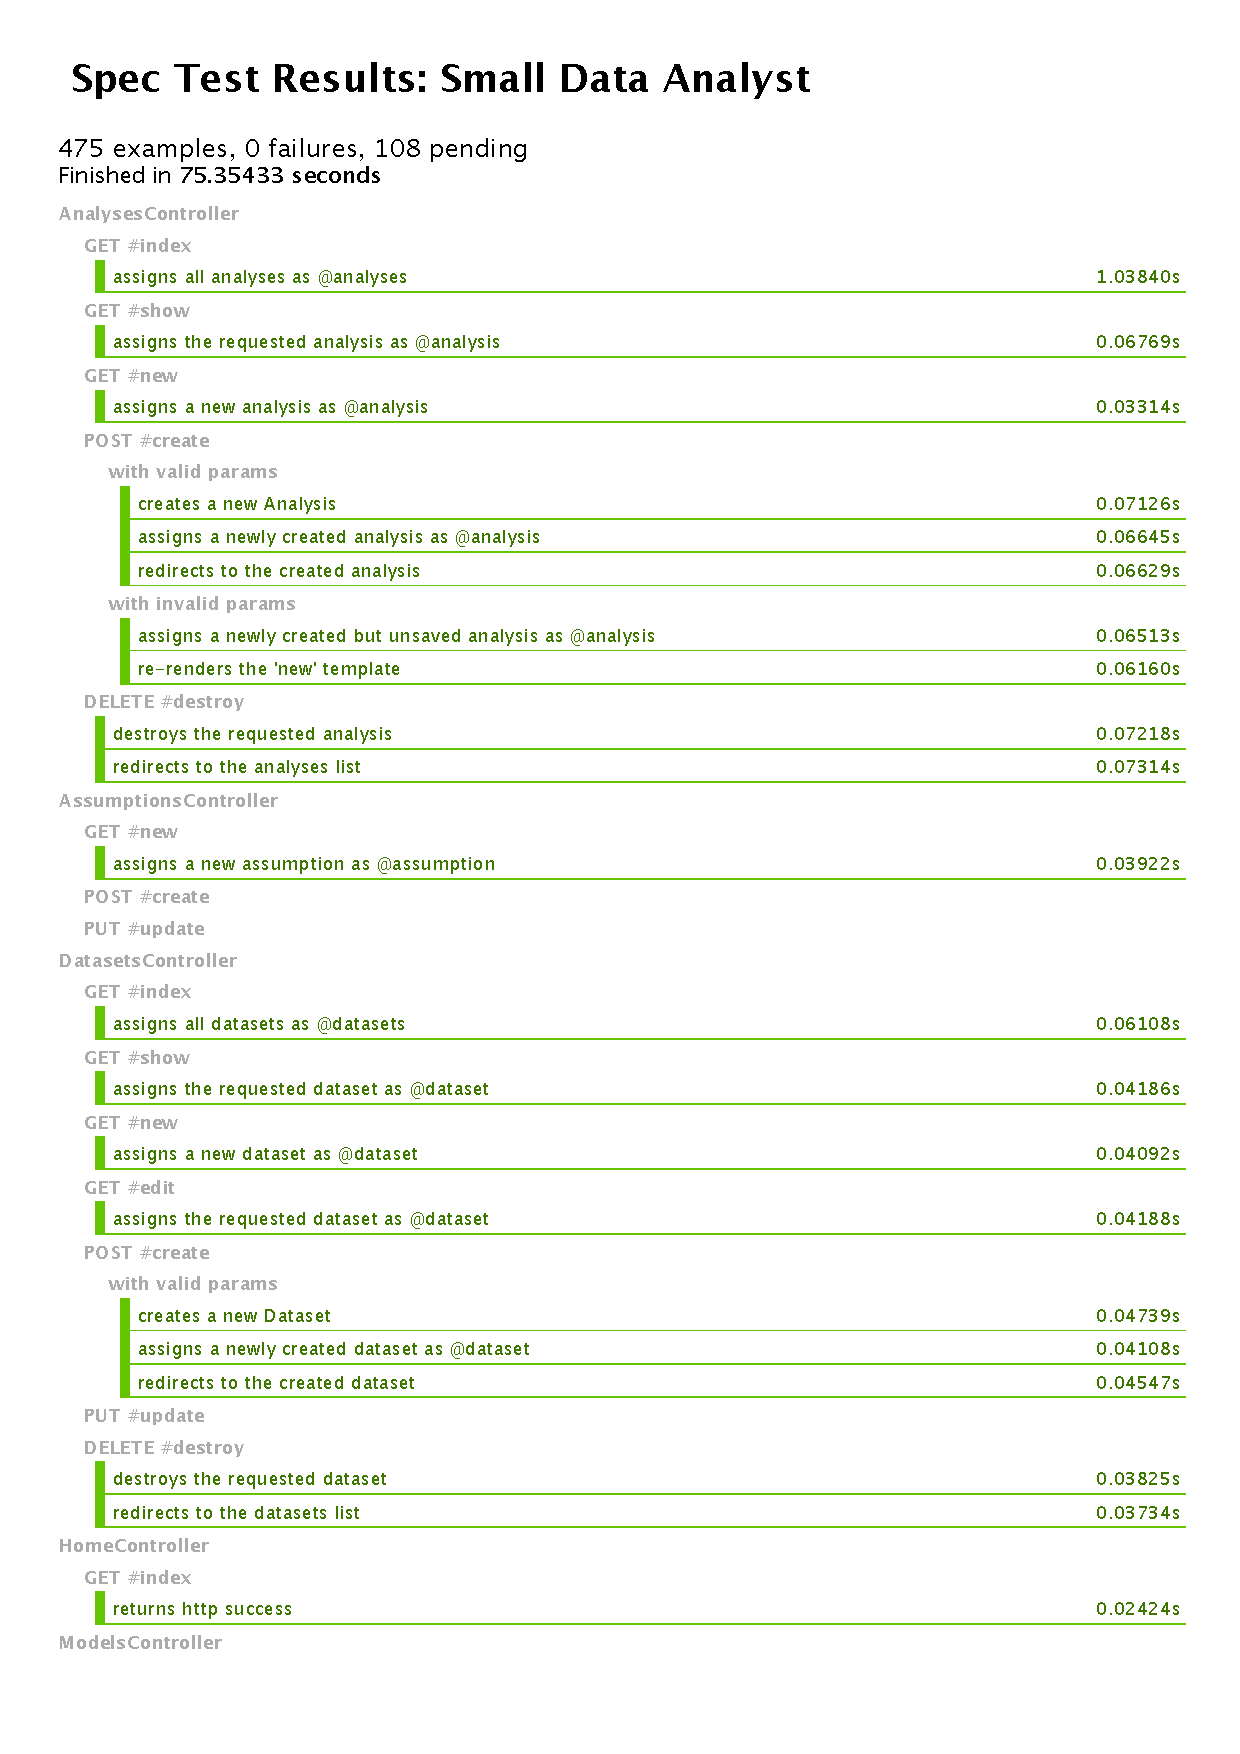
\includegraphics[page=1,width=0.5\textwidth]{appendix/RSpec}
	\includegraphics[page=2,width=0.5\textwidth]{appendix/RSpec}
	\caption{RSpec test suite export (example of the first two pages).}
	\label{sub:test_suit}
\end{sidewaysfigure}






%TC:endignore

\end{document}